% https://github.com/martinhelso/MathDept


\documentclass[UKenglish,8pt,aspectratio=1610]{beamer}

\usepackage[
backend=biber,        % compilateur par défaut pour biblatex
sorting=none,          % trier par nom, année, titre
citestyle=numeric, % style de citation auteur-année
bibstyle=numeric,  % style de bibliographie alphabétique
]{biblatex}
\addbibresource{biblio.bib}


\usetheme[NoLogo]{MathDept}

\usepackage{varwidth}
\usepackage[utf8]{inputenx} % For æ, ø, å
\usepackage{babel}          % Automatic translations
\usepackage{csquotes}       % Quotation marks
\usepackage{microtype}      % Improved typography
\usepackage{amssymb}        % Mathematical symbols
\usepackage{mathtools}      % Mathematical symbols
\usepackage[absolute, overlay]{textpos} % Arbitrary placement
\setlength{\TPHorizModule}{\paperwidth} % Textpos units
\setlength{\TPVertModule}{\paperheight} % Textpos units
\usepackage{tikz}
\usetikzlibrary{overlay-beamer-styles}  % Overlay effects for TikZ
\usepackage{dsfont}
\usepackage{fontawesome5}
\author{Thomas Aussaguès}
\title{Mandatory exercise 1}
\subtitle{Angular spectrum approach and array pattern}
\usepackage{siunitx}
\usepackage{graphics}
\graphicspath{{../jupyter/images/ASA},{../jupyter/images/array}}	

\usepackage{color}
\usepackage{colortbl}
\definecolor{darkred}{rgb}{0.6,0.0,0.0}
\definecolor{darkgreen}{rgb}{0,0.50,0}
\definecolor{lightblue}{rgb}{0.0,0.42,0.91}
\definecolor{orange}{rgb}{0.99,0.48,0.13}
\definecolor{grass}{rgb}{0.18,0.80,0.18}
\definecolor{pink}{rgb}{0.97,0.15,0.45}

% listings
\usepackage{listings}

% Python style for highlighting
\usepackage{booktabs}
\usepackage{multirow}

\begin{document}

\renewcommand{\arraystretch}{1.3}	
	
	
	% General Setting of listings
	\lstset{
		aboveskip=1em,
		breaklines=true,
		abovecaptionskip=-6pt,
		captionpos=b,
		escapeinside={\%*}{*)},
		frame=single,
		numbers=left,
		numbersep=15pt,
		numberstyle=\tiny,
	}
	% 0. Basic Color Theme
	\lstdefinestyle{colored}{ %
		basicstyle=\ttfamily,
		backgroundcolor=\color{gray},
		commentstyle=\color{green}\itshape,
		keywordstyle=\color{blue}\bfseries\itshape,
		stringstyle=\color{red},
	}
	% 1. General Python Keywords List
	\lstdefinelanguage{PythonPlus}[]{Python}{
		morekeywords=[1]{,as,assert,nonlocal,with,yield,self,True,False,None,} % Python builtin
		morekeywords=[2]{,__init__,__add__,__mul__,__div__,__sub__,__call__,__getitem__,__setitem__,__eq__,__ne__,__nonzero__,__rmul__,__radd__,__repr__,__str__,__get__,__truediv__,__pow__,__name__,__future__,__all__,}, % magic methods
		morekeywords=[3]{,object,type,isinstance,copy,deepcopy,zip,enumerate,reversed,list,set,len,dict,tuple,range,xrange,append,execfile,real,imag,reduce,str,repr,}, % common functions
		morekeywords=[4]{,Exception,NameError,IndexError,SyntaxError,TypeError,ValueError,OverflowError,ZeroDivisionError,}, % errors
		morekeywords=[5]{,ode,fsolve,sqrt,exp,sin,cos,arctan,arctan2,arccos,pi, array,norm,solve,dot,arange,isscalar,max,sum,flatten,shape,reshape,find,any,all,plot,linspace,legend,quad,polyval,polyfit,hstack,concatenate,vstack,column_stack,empty,zeros,ones,rand,vander,grid,pcolor,eig,eigs,eigvals,svd,qr,tan,det,logspace,roll,min,mean,cumsum,cumprod,diff,vectorize,lstsq,cla,eye,xlabel,ylabel,squeeze,correlate,argmax,abs,np.}, % numpy / math
	}
	% 2. New Language based on Python
	\lstdefinelanguage{PyBrIM}[]{PythonPlus}{
		emph={d,E,a,Fc28,Fy,Fu,D,des,supplier,Material,Rectangle,PyElmt},
	}
	% 3. Extended theme
	\lstdefinestyle{colorEX}{
		basicstyle=\ttfamily,
		backgroundcolor=\color{gray!10},
		commentstyle=\color{darkgreen}\slshape,
		keywordstyle=\color{blue}\bfseries\itshape,
		keywordstyle=[2]\color{blue}\bfseries,
		keywordstyle=[3]\color{grass},
		keywordstyle=[4]\color{red},
		keywordstyle=[5]\color{orange}\bfseries,
		stringstyle=\color{darkred},
		emphstyle=\color{pink}\underbar,
	}
	
	
	\begin{frame}{Table of contents}
		\tableofcontents
	\end{frame}
	
	\section{Angular Spectrum Approach}
	\subsection{Unfocused ASA simulation}
	\begin{frame}
		\frametitle{\textsc{GIBBS} phenomenon 1}
		
				\begin{columns}
			\begin{column}{0.5\textwidth}
				
					\vspace{-15pt}
				\begin{figure}[h!]
					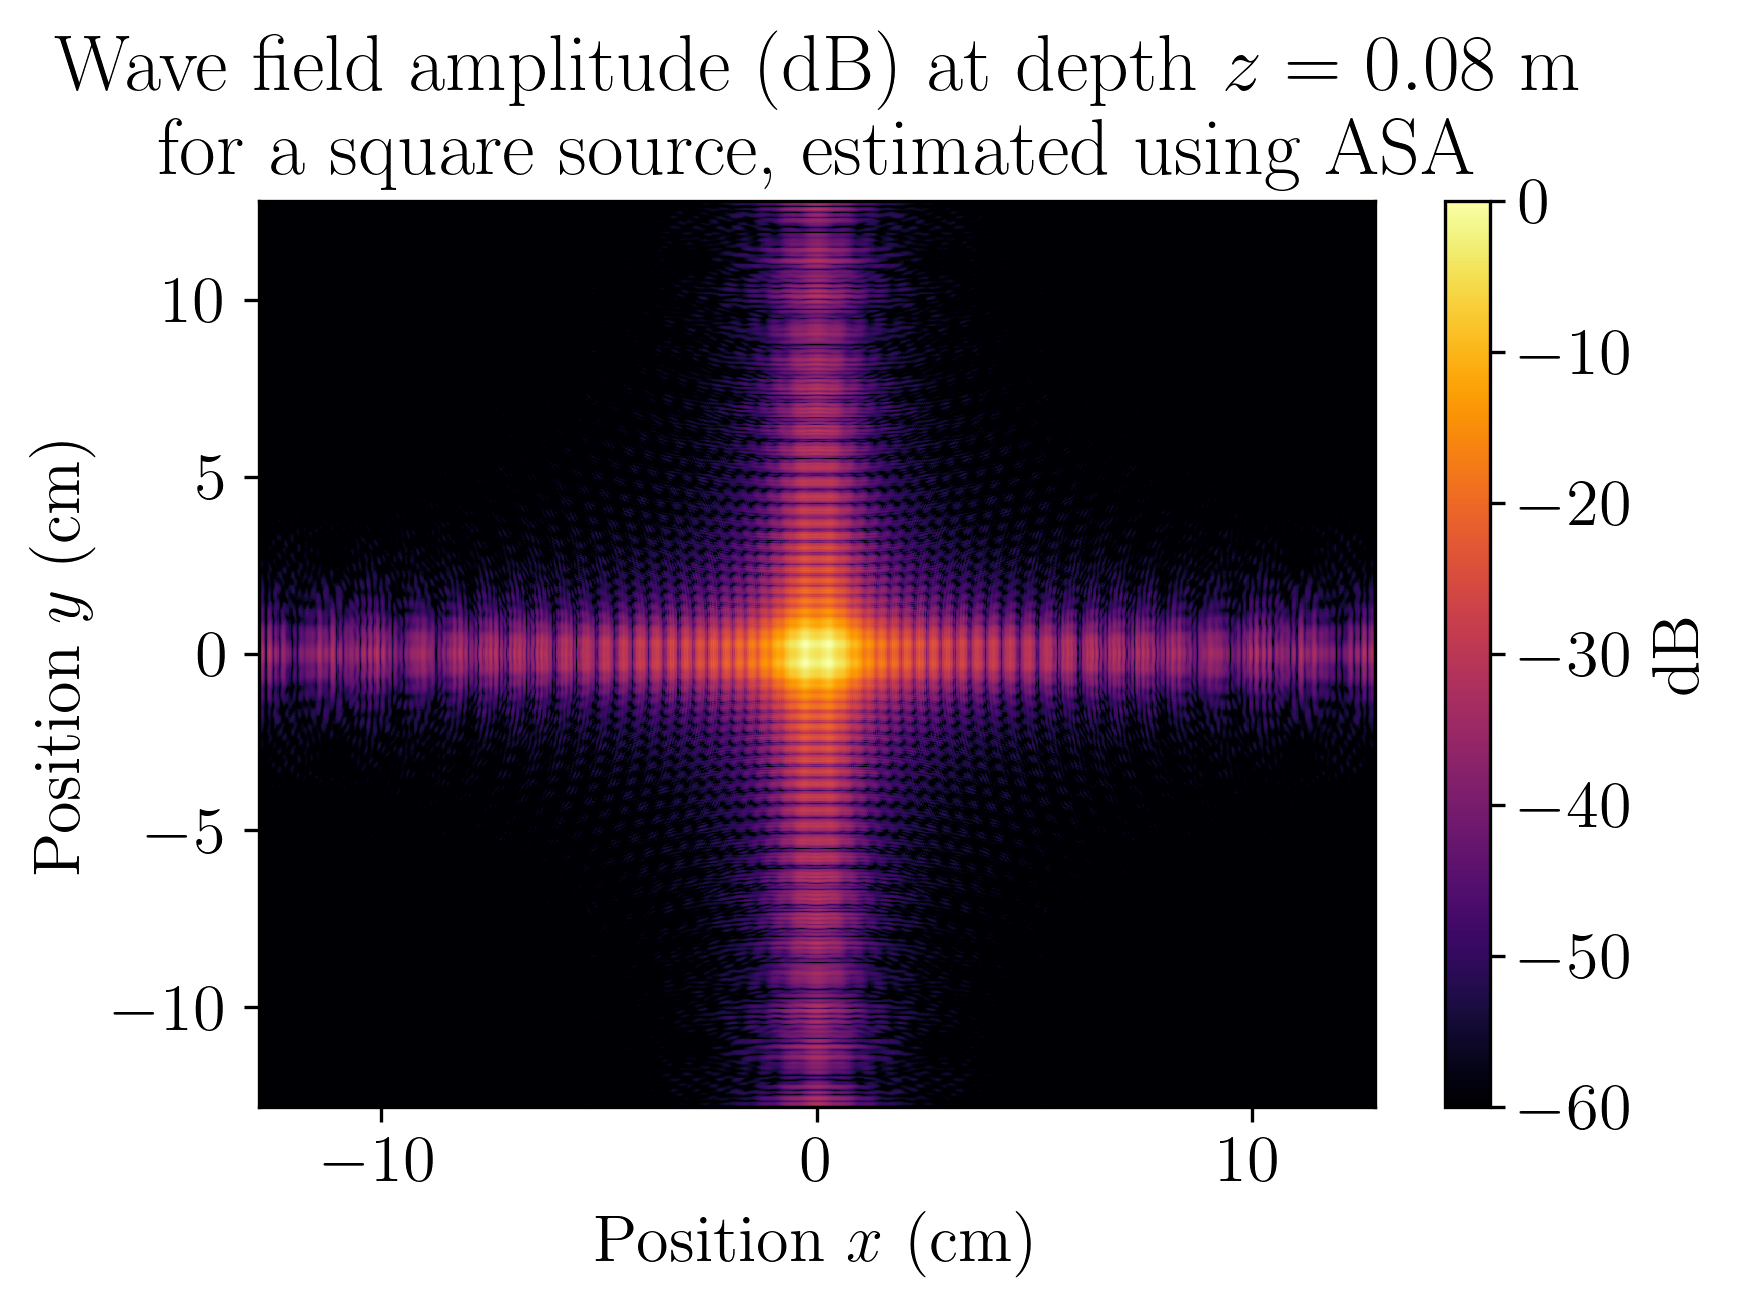
\includegraphics[scale=0.35]{square/wave_field_2D_z=8cm_square.png}
					\centering
					\vspace{-5pt}
					\caption{Wave field at $z=0.08~\si{\meter}$}
				\end{figure}
				\vspace{-20pt}
				\begin{figure}[h!]
				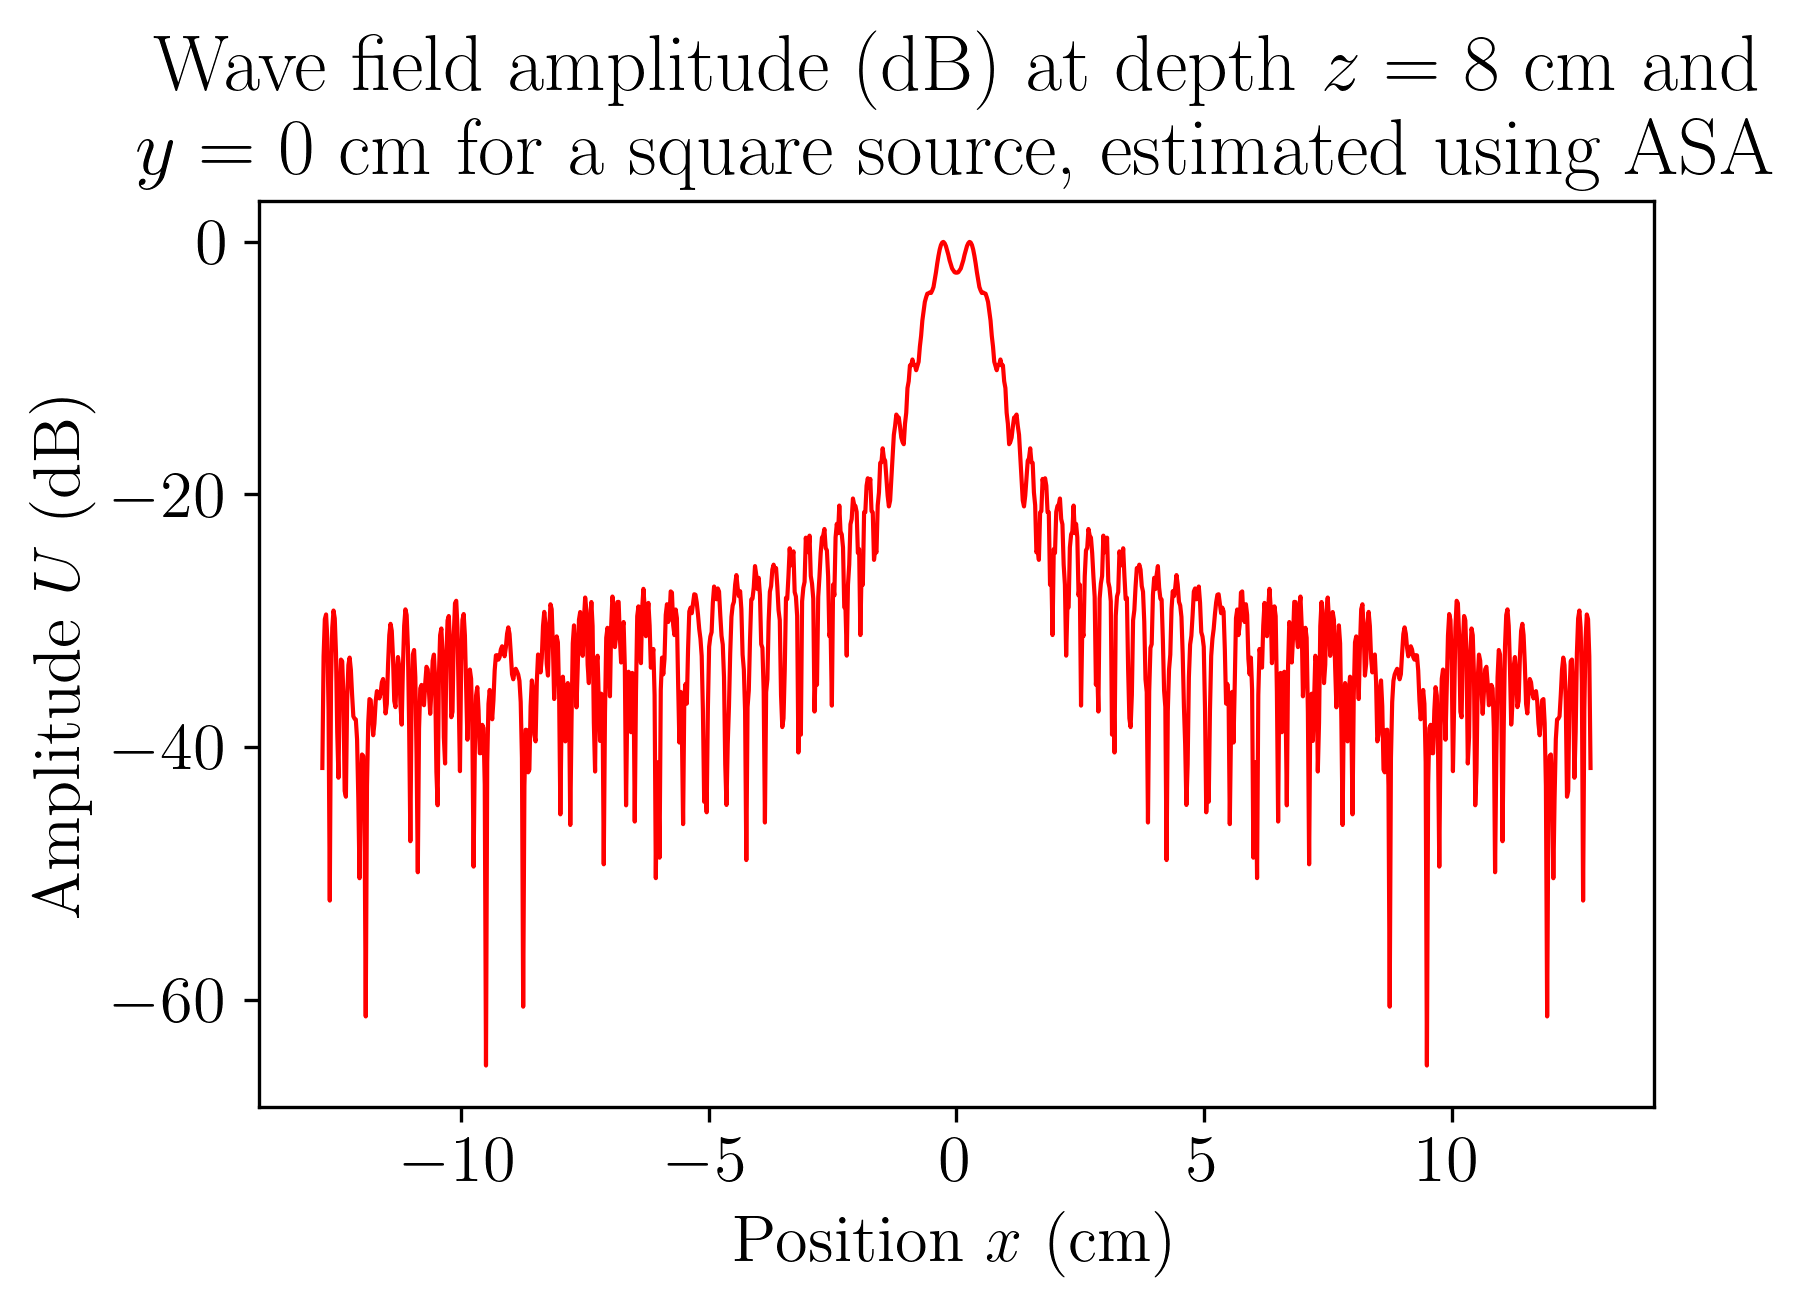
\includegraphics[scale=0.35]{square/wave_field_1D_z=8cm_square.png}
				\centering
				\vspace{-5pt}
				\caption{Center cut of the wave field at $z=0.08~\si{\meter}$}
			\end{figure}
		
			\end{column}
			\begin{column}{0.5\textwidth}
				
				\begin{figure}[h!]
					\vspace{-35pt}
				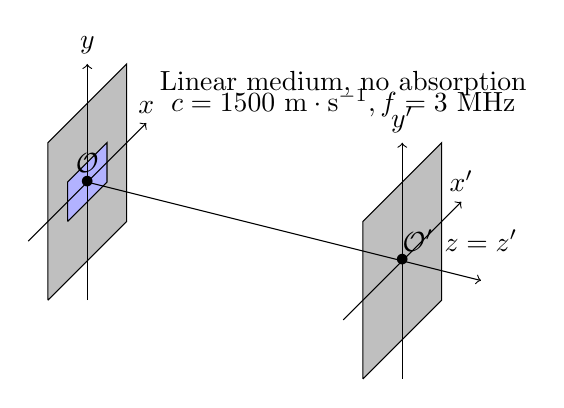
\begin{tikzpicture}
					
					
					%\draw[step=0.25,black,thin] (-5,-2) grid (2,3);
					
					\draw [fill=gray!50](-4.5,-1.5)--(-3.5,-0.5)--(-3.5,1.5)--(-4.5,0.5)--(-4.5,-1.5);
					\draw [fill=blue!30] (-4.25,-0.5)--(-3.75,0)--(-3.75,0.5)--(-4.25,0)--(-4.25,-0.5);
					
					\draw (-4,0) node {$\bullet$};
					\draw (-4,0) node [above] {$\mathcal{O}$};
					\draw [->] (-4.75,-0.75)--(-3.25,0.75);
					\draw [->] (-4,-1.5)--(-4,1.5);
					\draw (-3.25,0.75) node [above] {$x$};
					\draw (-4,1.5) node [above] {$y$};
					
					
					
					
					
					
					
					
					\draw (-0.75,1.25) node {Linear medium, no absorption};
					\draw (-0.75,1) node {$c=1500~\si{\meter\cdot\second^{-1}},f=3~\si{\mega\hertz}$};
				
				
					\draw [fill=gray!50](-.5,-2.5)--(.5,-1.5)--(.5,.5)--(-.5,-.5)--(-.5,-2.5);
					\draw (0.2,-1) node [above] {$\mathcal{O}'$};
					\draw [->] (-4,0)--(1,-1.25);
					\draw (1,-1) node [above]  {$z=z'$};
					
						\draw [->] (-.75,-1.75)--(0.75,-0.25);
					\draw [->] (0,-2.5)--(0,0.5);
					\draw (0.75,-.25) node [above] {$x'$};
					\draw (0,0.5) node [above] {$y'$};
					\draw (0,-1) node {$\bullet$};
					
					
					
				
					
				
				\end{tikzpicture}
			\centering
			\caption{Geometry}
				\end{figure}
			\vspace{-10pt}
				\begin{itemize}
					\item Energy located at the wave field center and along the $x$ and $y$-axis 
					\item Square aperture $U$ ($15\times 15\lambda^2$) %: distribution at depth $z$ $\approx \mathrm{sinc}\left(x\right)\mathrm{sinc}\left(y\right)$ 
					\item Very low side lobes ! 
					\item Here, \textbf{\textcolor{red}{energy outside}} the wave field center\dots Why ?
					\item \textsc{GIBBS} phenomenon : we are trying to approximate a \textbf{\textcolor{red}{discontinuous}} function by a \textbf{\textcolor{red}{finite}} sum of continuous functions
					\item $\implies$ oscillations and artefacts, energy is spread outside the center
					\item \textcolor{red}{\textbf{How to make the aperture continuous ?}}
				\end{itemize}
			\end{column}
		\end{columns} 
		
	\end{frame}
	
	\begin{frame}
		\frametitle{\textsc{GIBBS} phenomenon 2}
		
			\begin{columns}
			\begin{column}{0.5\textwidth}
					\vspace{-20pt}
					\begin{figure}[h!]
					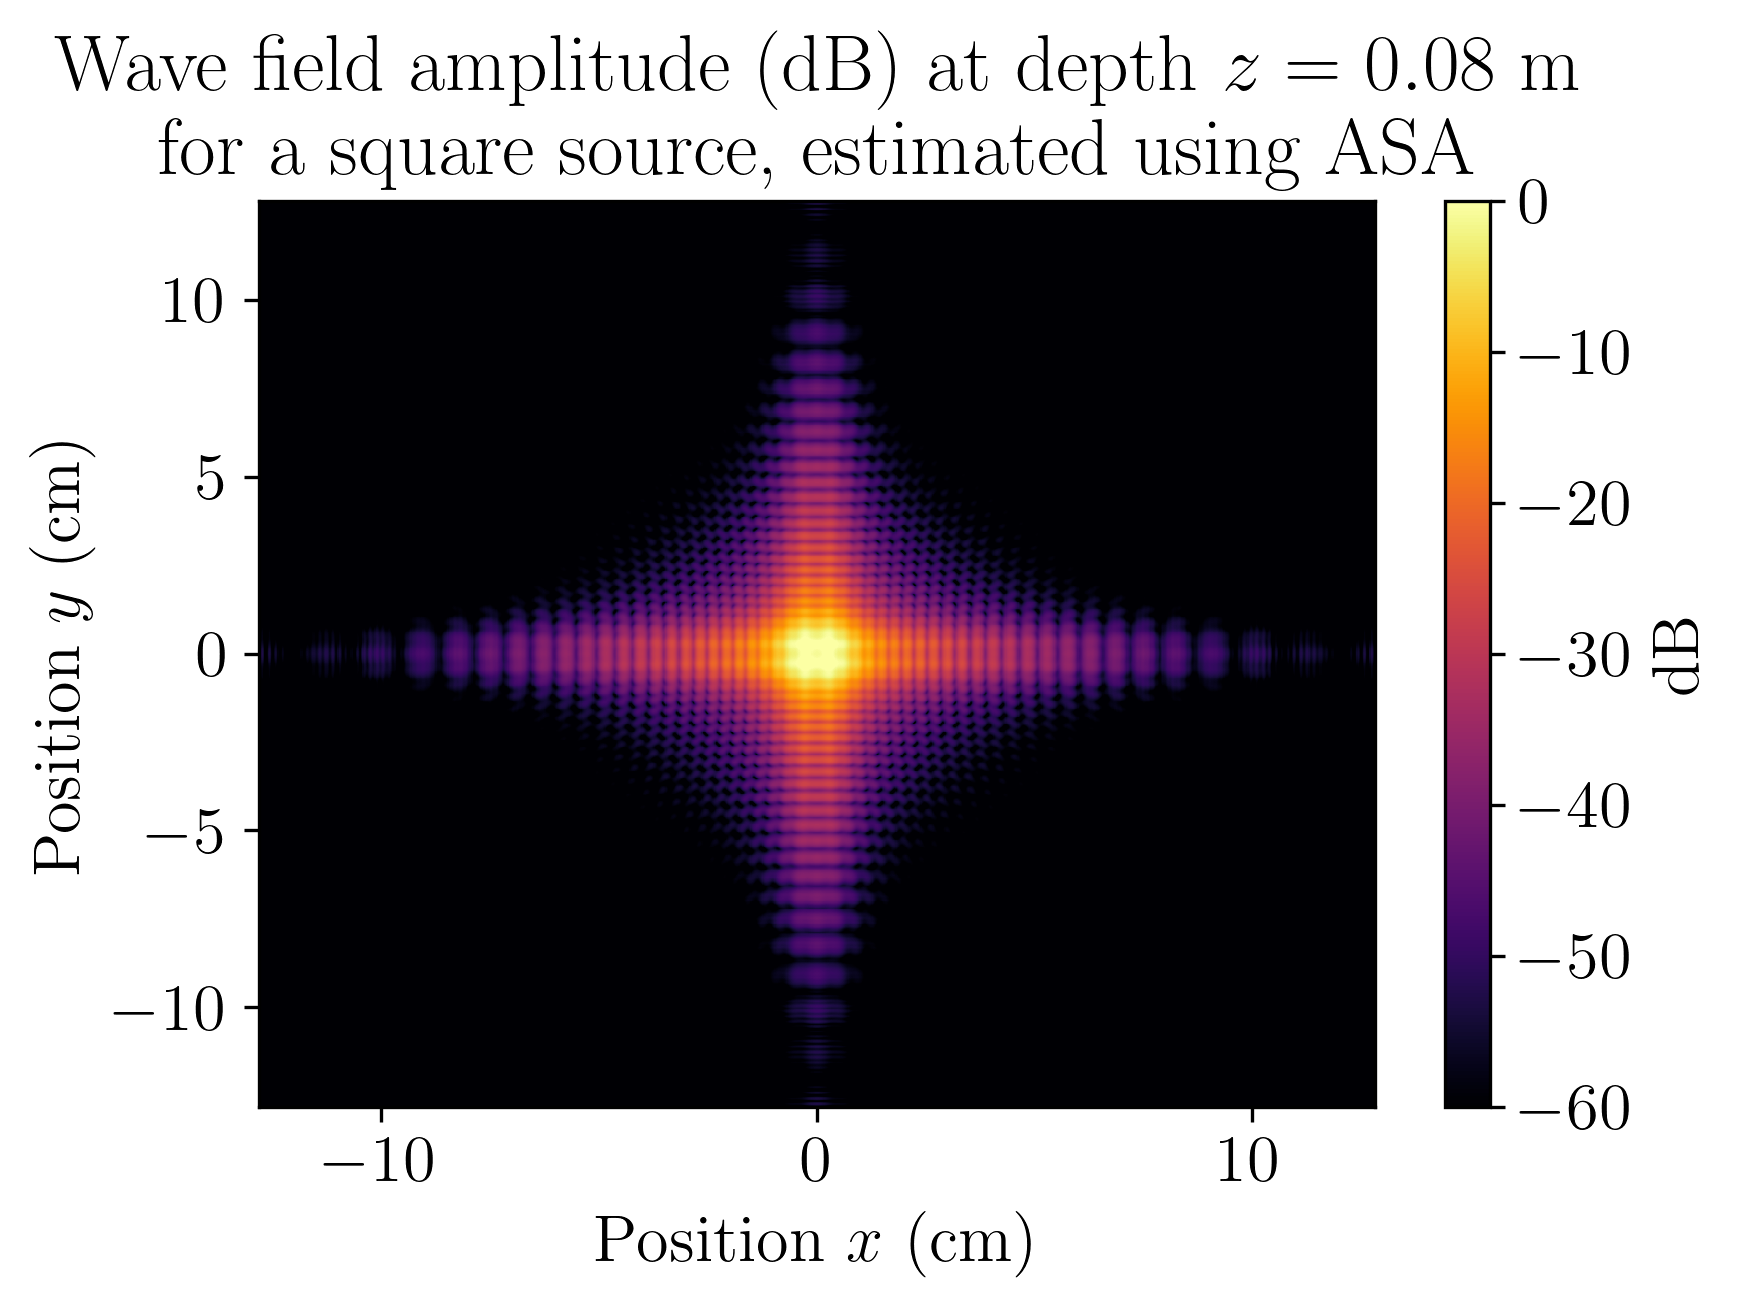
\includegraphics[scale=0.35]{square/wave_field_2D_z=8cm_square_smoothed.png}
					\centering
					\caption{Wave field at $z=0.08~\si{\meter}$ (smoothed aperture)}
						\vspace{-10pt}
				\end{figure}
				\begin{itemize}
				\item How to make the jump  from 0 to 1 at $x,y=r$ \textcolor{red}{\textbf{continuous}} ?
				\item \textsc{Hanning} window $\mathcal{H}\longleftrightarrow$ filter : new aperture $U_{mod}=\mathcal{H}\star U$
				\item The new aperture is \textbf{\textcolor{red}{continuous}} !
				\item Energy located at the wave field center
				\item Lower side lobes : $-20~\si{\decibel}\implies$ reduced artefacts 
				\item Smoother curve
				\item Same remarks with a circular aperture (except that the observed image should be a \textsc{BESSEL} function $J_1$ in the far field)
				
			\end{itemize}
			\end{column}
			\begin{column}{0.51\textwidth}
				\vspace{-20pt}
				\begin{figure}[h!]
					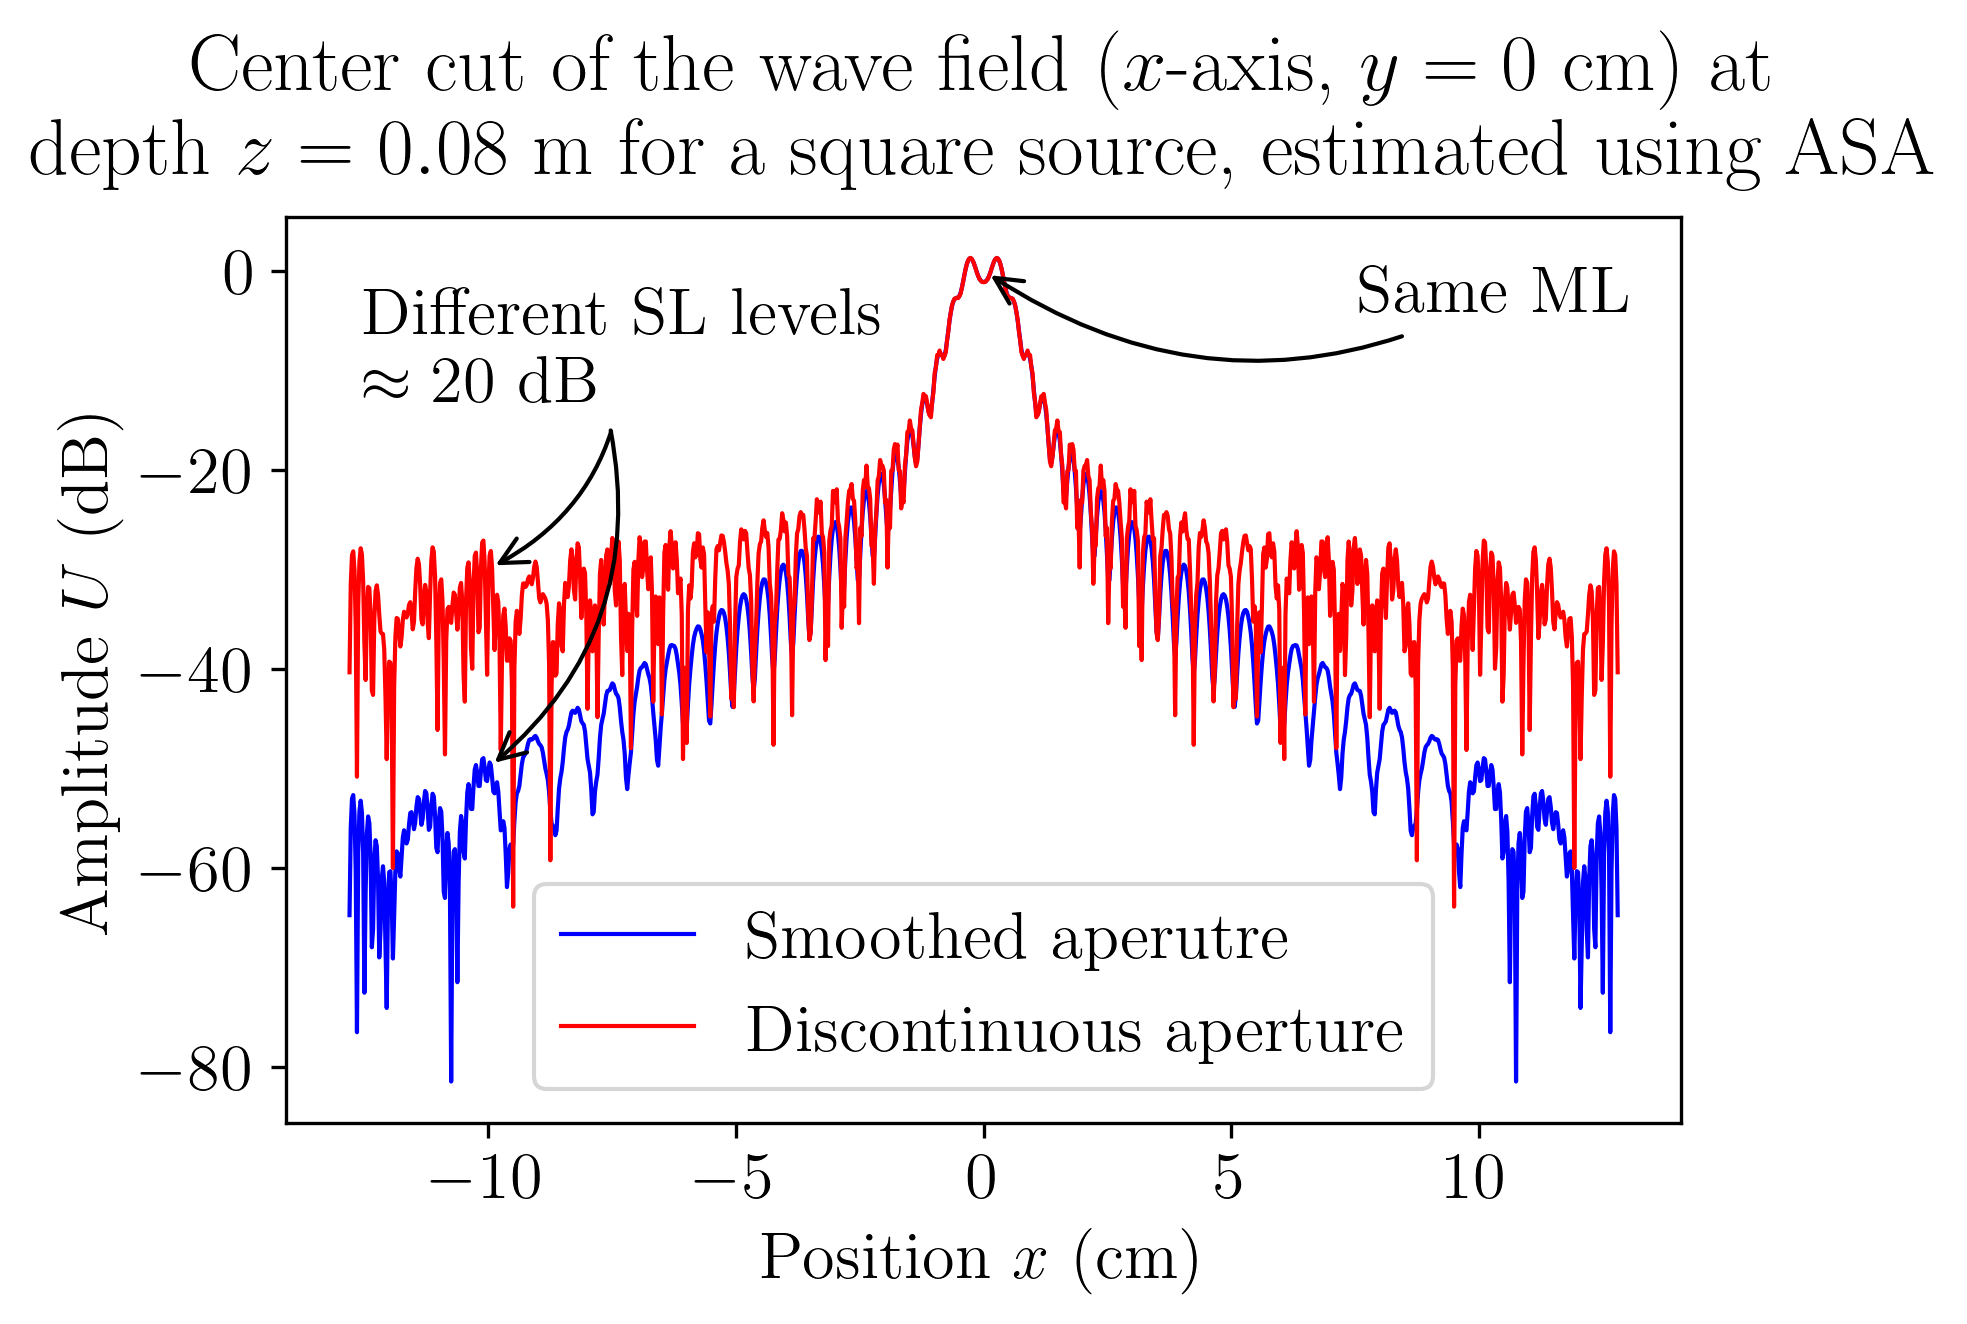
\includegraphics[scale=0.35]{square/wave_field_1D_z=8cm_square_smoothed_vs_normal.png}
					\centering
					\caption{Center cut of the wave field at $z=0.08~\si{\meter}$}
				\end{figure}
			\vspace{-20pt}
			\begin{figure}
				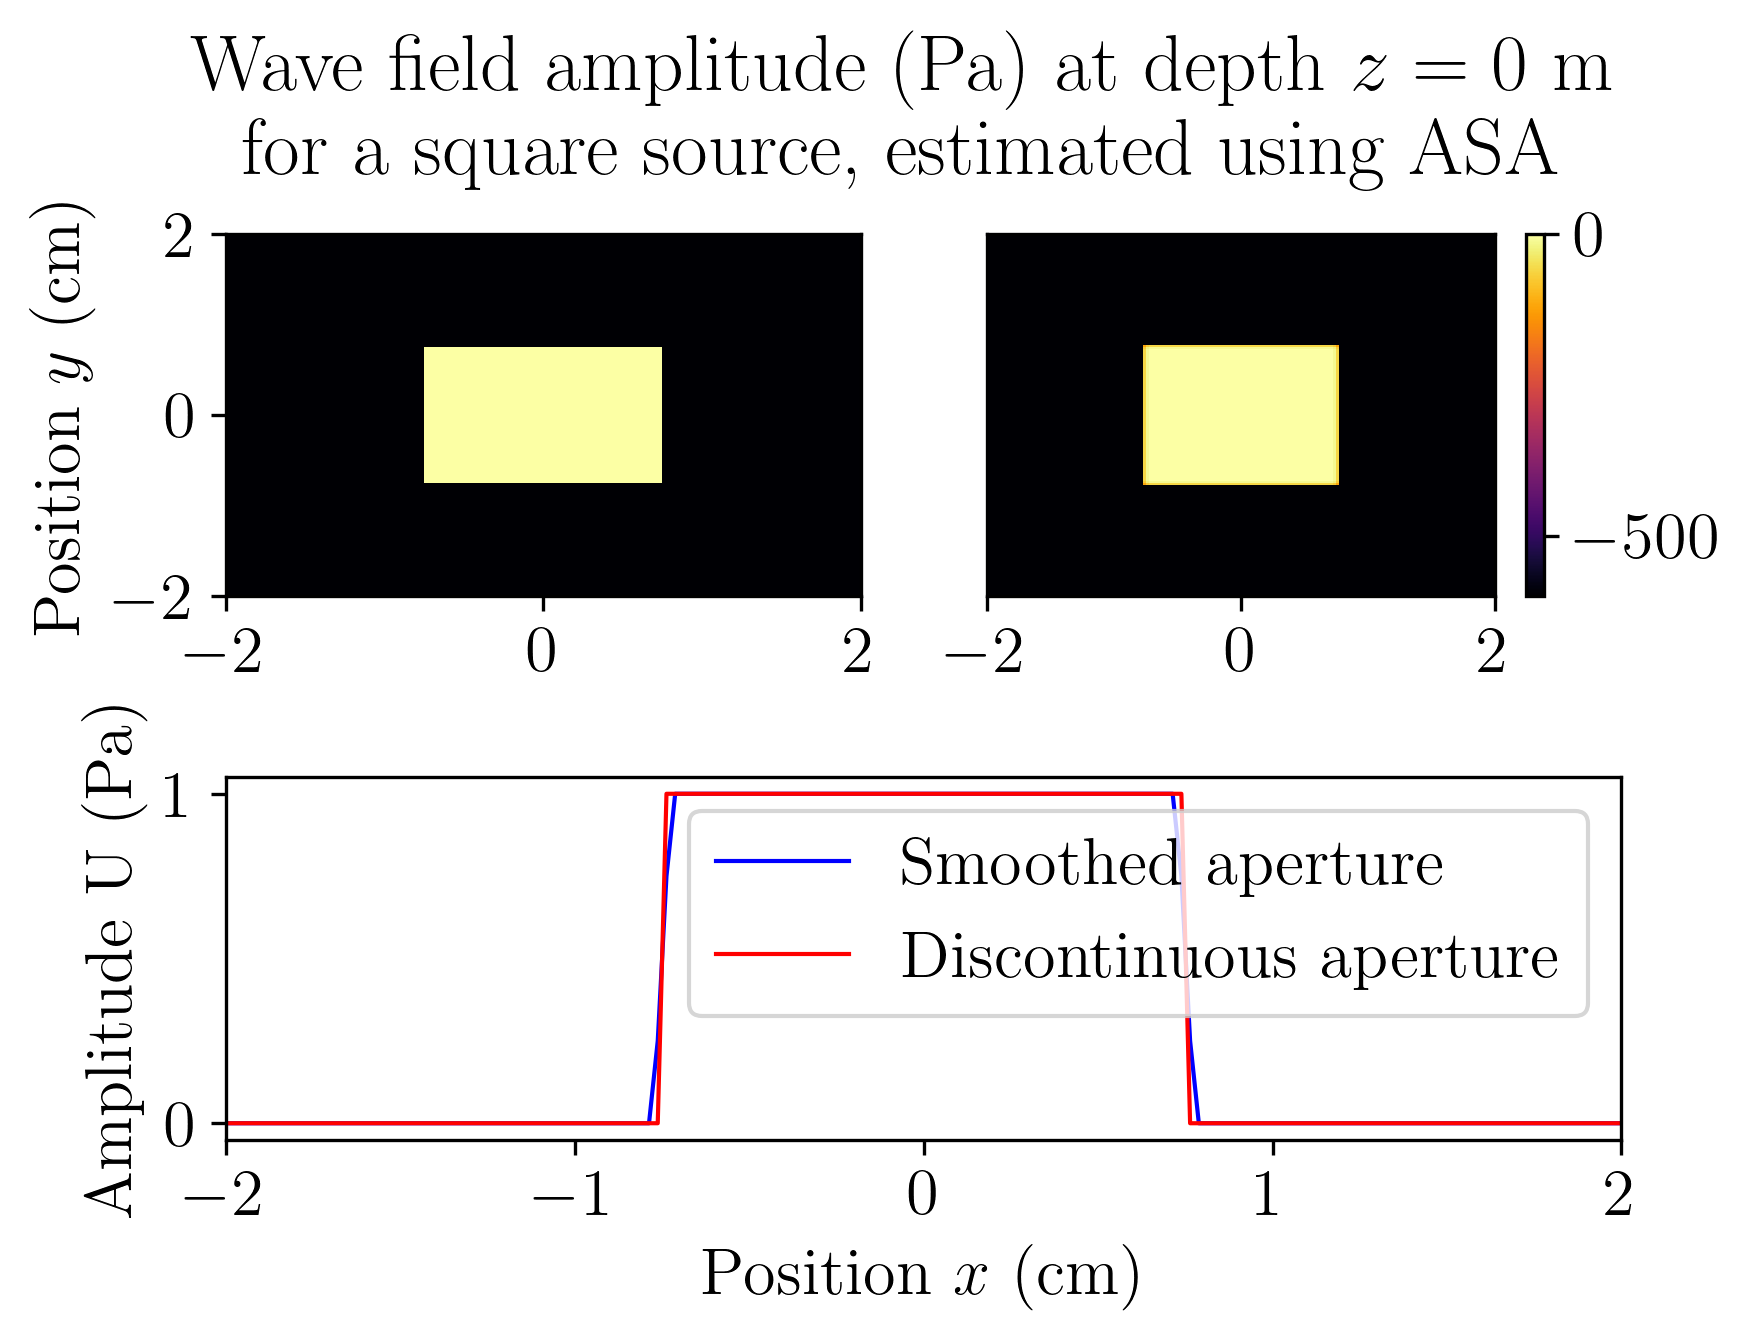
\includegraphics[scale=0.35]{square/wave_field_2D_z=0_square_smoothed_vs_normal.png}
				\centering
				\caption{Effect of the \textsc{HANNING} window}
			\end{figure}
			\end{column}
		\end{columns}
				
			
		
			
	
	
	\end{frame}

	\begin{frame}
		\frametitle{Near field vs. far field 1}
		\begin{itemize}
			\item \textbf{Near field}\footnote{For a circular source, or we have a square source here\dots} : $\lambda \leq \frac{D^2}{4\lambda}=\frac{(2\times15\lambda)^2}{4\lambda}=225\lambda=~0.11\si{\meter}$, \textbf{\textcolor{red}{superposition}} of an infinite number of spherical waves with different phases : interferences
			\item \textbf{Far field} : $\lambda \geq \frac{D^2}{\lambda}=900\lambda=0.45~\si{\meter}$ : \textbf{\textcolor{red}{superposition}} of  an infinite number of plane waves with same phases : constructive interferences
			\item Limit ? Check if the amplitude is varying along the $x$-axis
		\end{itemize}
		\begin{columns}
		\begin{column}{0.5\textwidth}
			
			\vspace{-15pt}
			\begin{figure}[h!]
				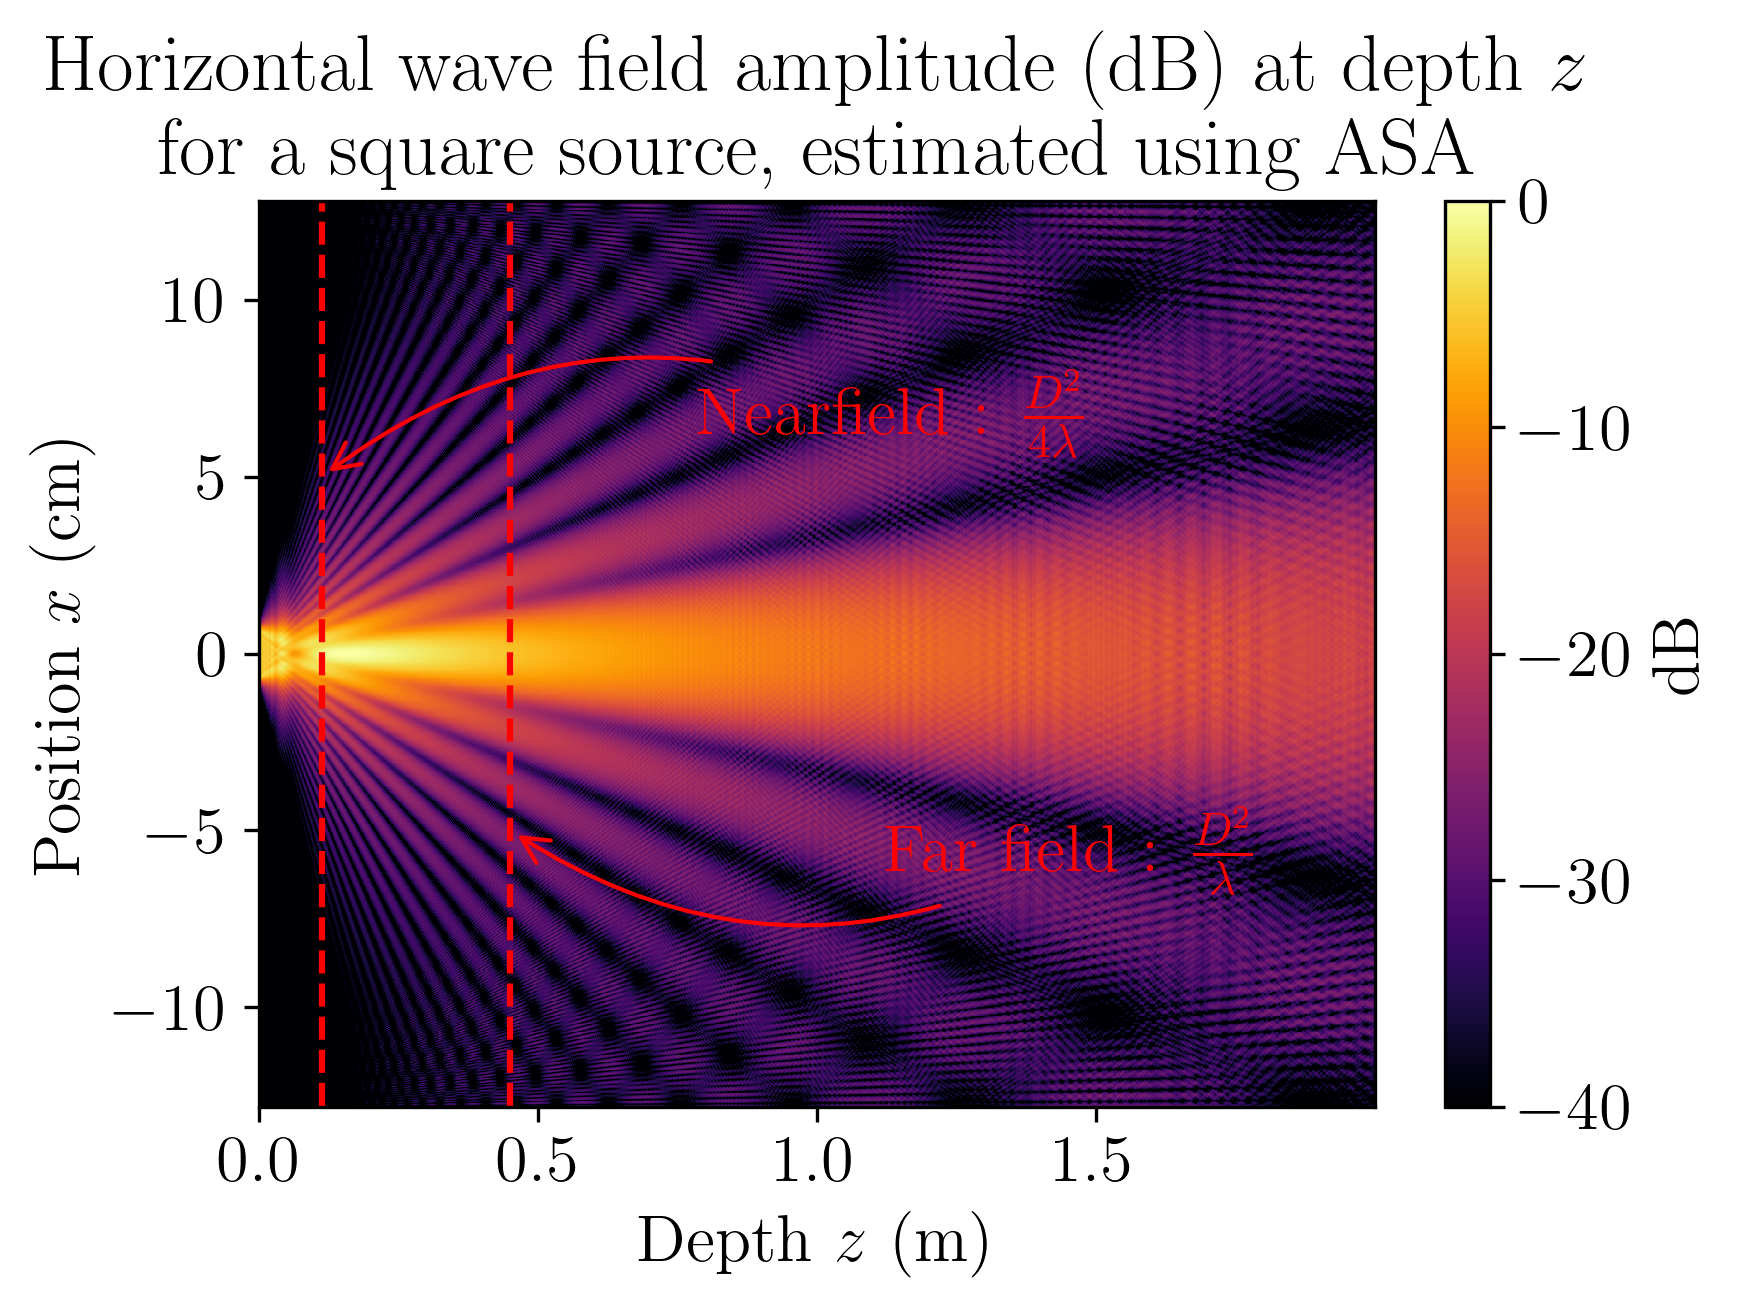
\includegraphics[scale=0.35]{square/wave_field_2D_xz_square_smoothed.png}
				\centering
					\vspace{-7pt}
				\caption{2D image of the predicted wave field for $y = 0~\si{\meter}$}
					\vspace{-8pt}
			\end{figure}
		\end{column}
		\begin{column}{0.5\textwidth}
			\vspace{-15pt}
			\begin{figure}[h!]
				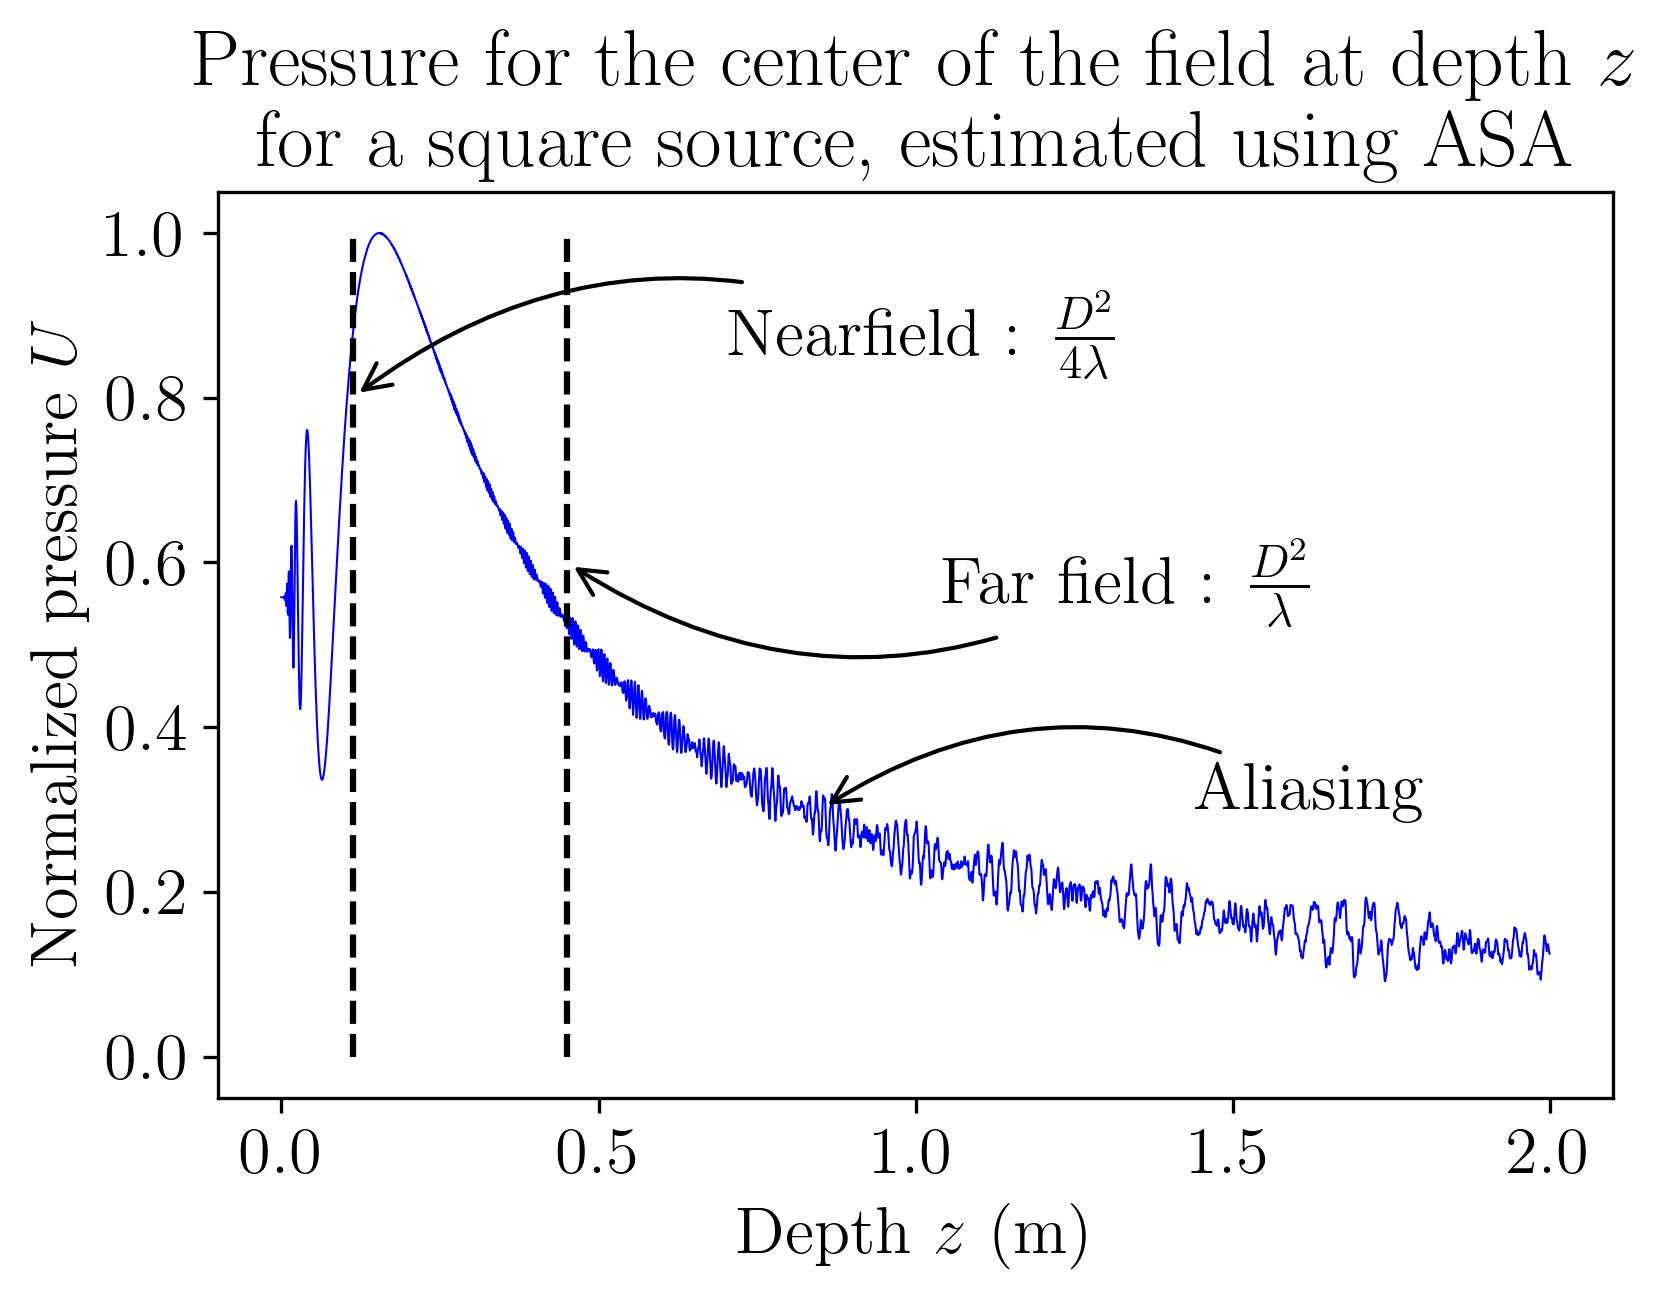
\includegraphics[scale=0.35]{square/wave_field_1D_center_square_smoothed.png}
				\centering
					\vspace{-7pt}
				\caption{Pressure at the wave field center}
					\vspace{-8pt}
			\end{figure}

		\end{column}
		\end{columns}
		\begin{itemize}
		\item \textbf{Near field} : oscillations for the amplitude (transitional regime)
		\item \textbf{Far field} : amplitude uniform inside a "small" plane $xy$, approximation of a spherical surface by a plane, amplitude $\propto \frac{1}{r}$, coherent with the spherical wave equation solution $U(\vec{r},t)=U_0\frac{\exp(j(\omega t-\vec{k}\cdot\vec{r}))}{\rVert\vec{r}\rVert}$
		\item \textbf{\textcolor{red}{High frequency patterns : aliasing}}
		
	\end{itemize}
	\end{frame}

\begin{frame}
		\frametitle{Near field vs. far field 2}
		
		\begin{itemize}
			\item We can define a direction $\theta=\arctan\dfrac{x}{2z}$
			\item \textbf{Near field} : wave field varies along the $x$-axis, energy focused in the direction $\theta=0$, low side lobes 
			\item \textbf{Far field} : wave field "uniform" along the $x$-axis, for small values of $\theta$, paraxial approximation + aliasing\footnote{Due to the source replicas}
		\end{itemize}
			\begin{columns}
			\begin{column}{0.5\textwidth}
				
				\vspace{-15pt}
				\begin{figure}[h!]
					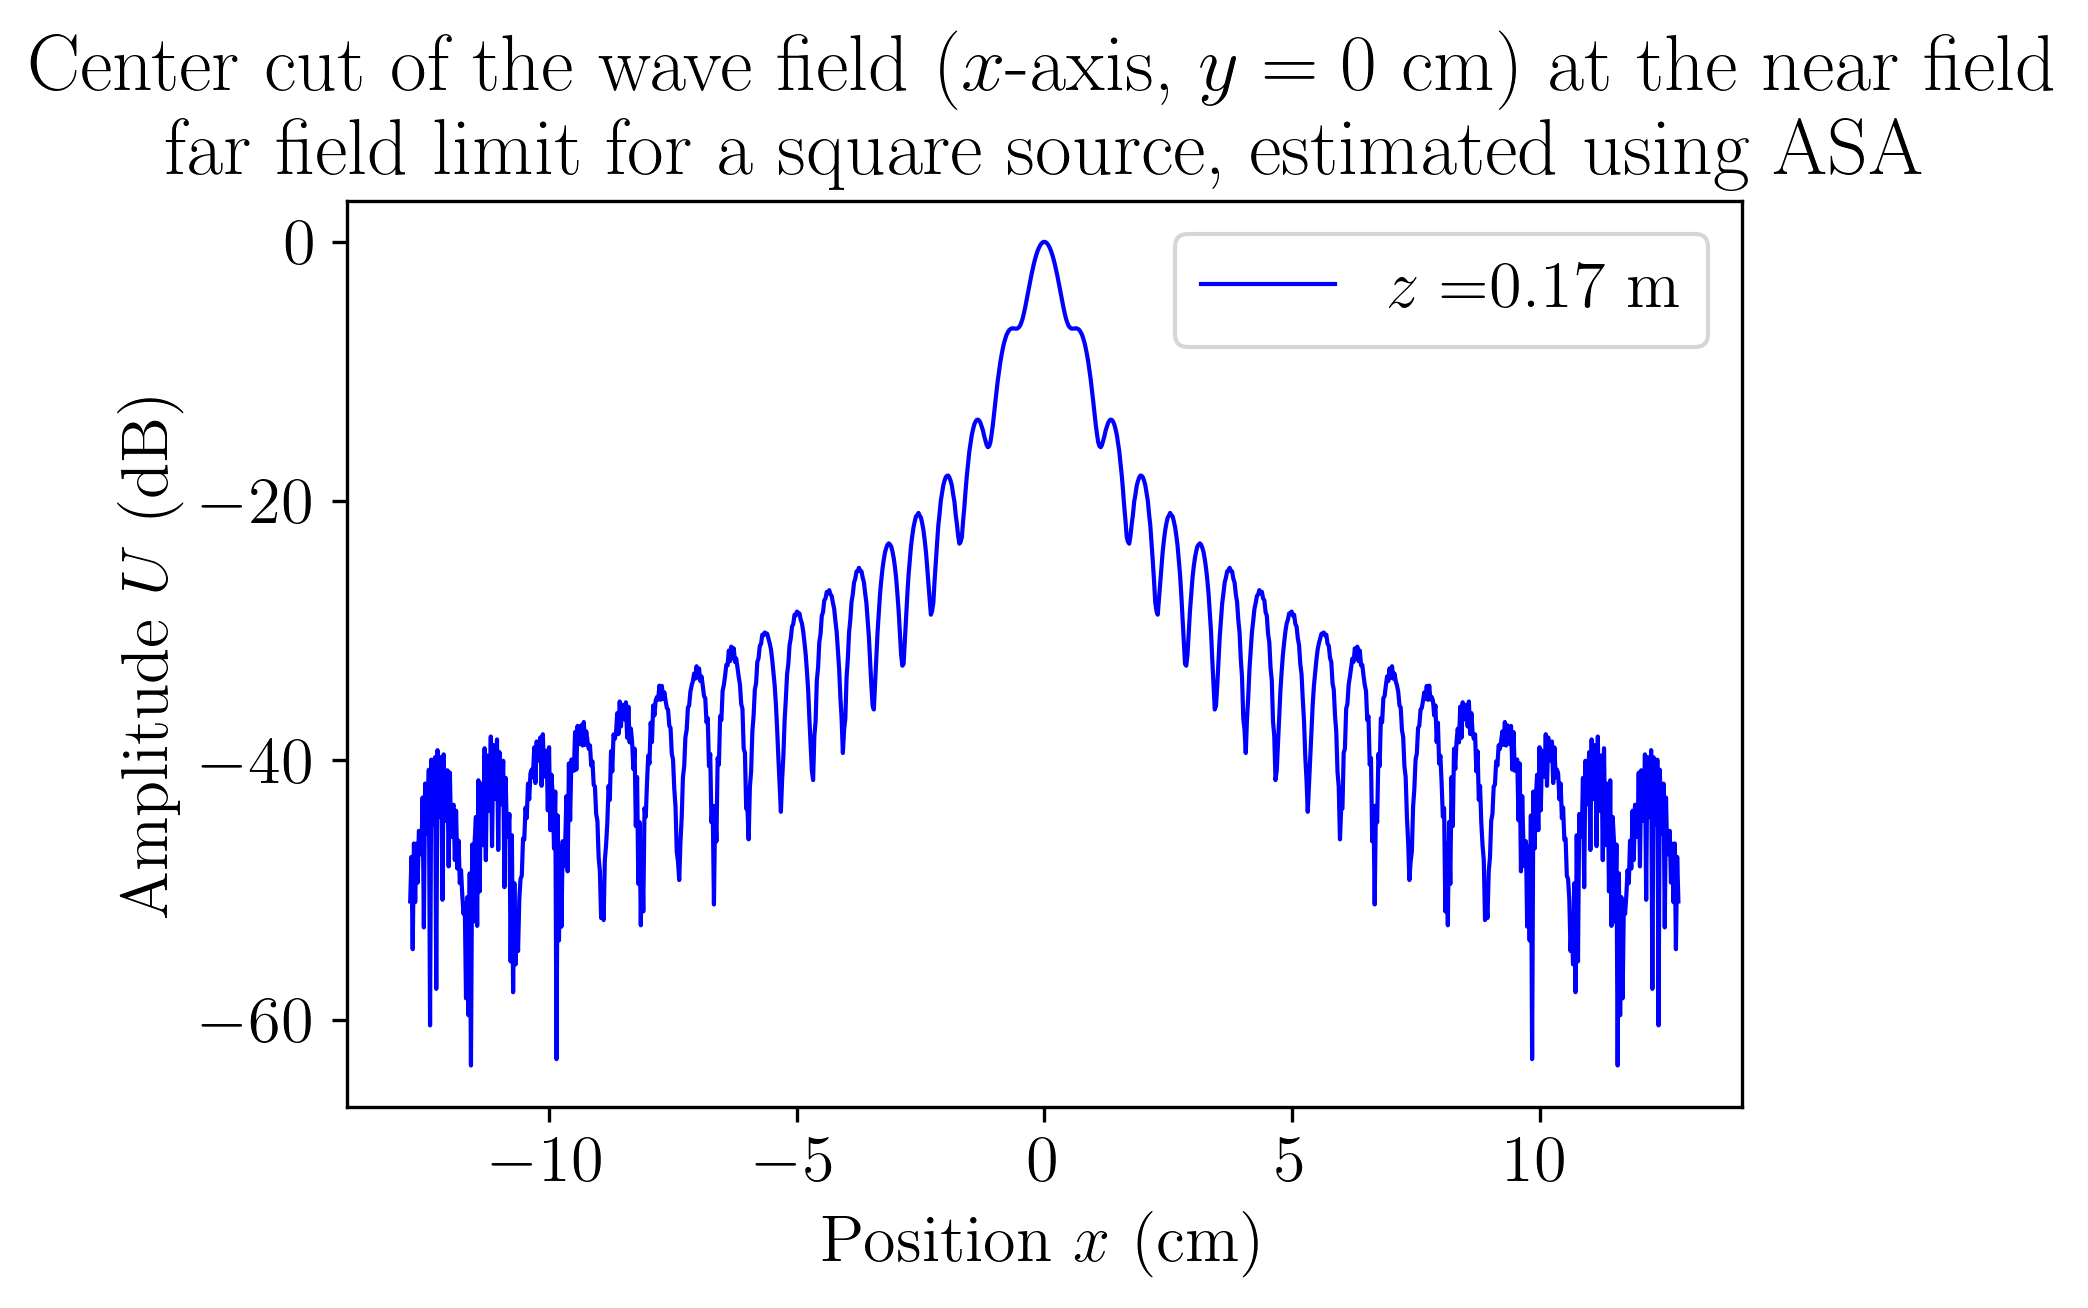
\includegraphics[scale=0.35]{square/wave_field_1D_near_far_limit_square_smoothed.png}
					\centering
					\caption{Wave field center cut at the near field far field limit}
				\end{figure}
			\end{column}
			\begin{column}{0.5\textwidth}
				\vspace{-15pt}
				\begin{figure}[h!]
					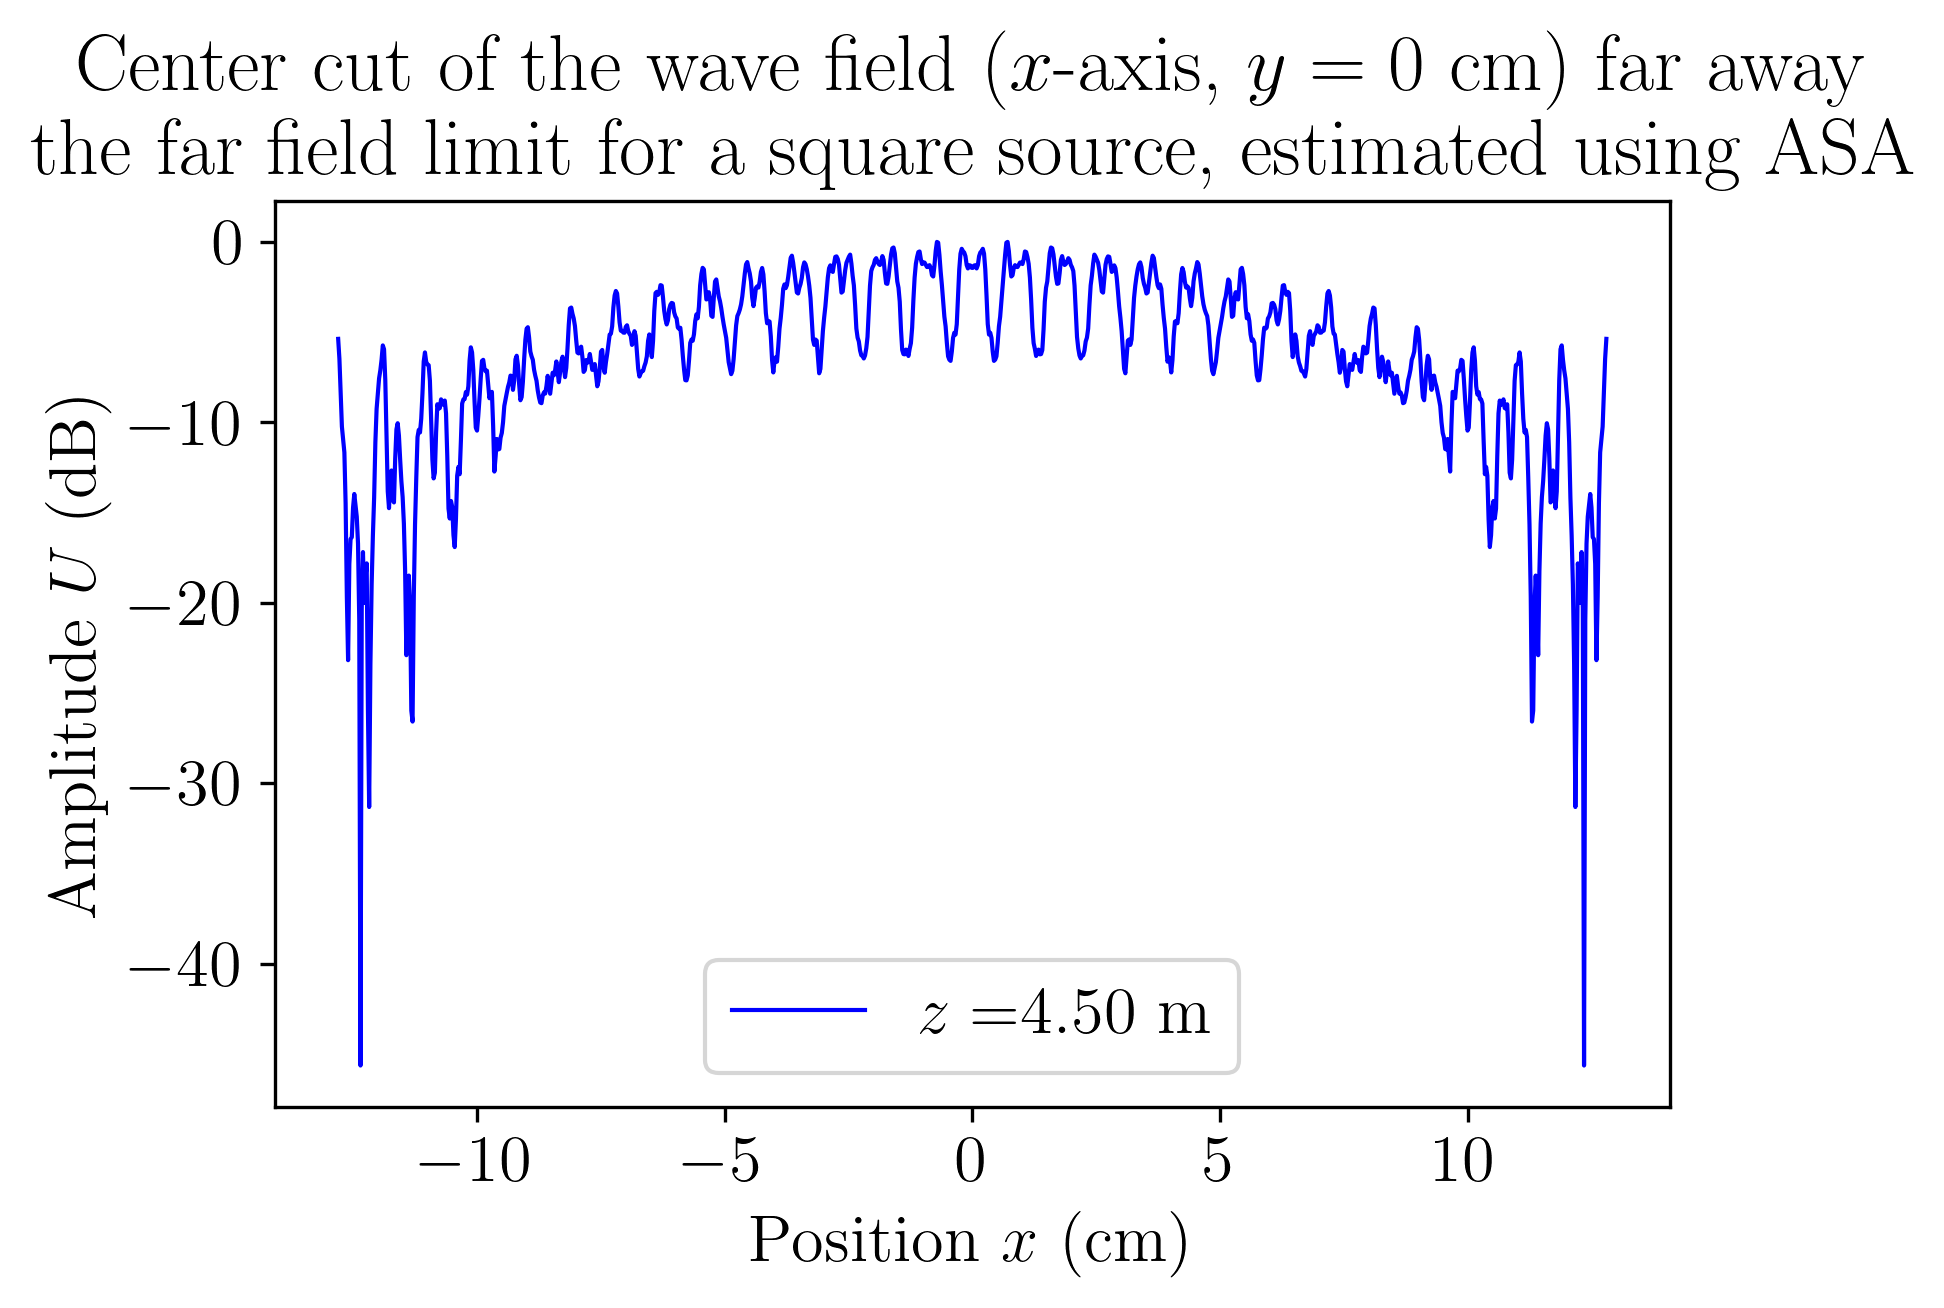
\includegraphics[scale=0.35]{square/wave_field_1D_far_limit_square_smoothed.png}
					\centering
					\caption{Wave field center cut at a range much larger than the near field far field limit}
				\end{figure}
				
			\end{column}
		\end{columns}
	
\end{frame}

	\subsection{Focused ASA simulation}
	
	\begin{frame}
		\frametitle{Focused ASA simulation}
		\begin{itemize}
			\item \textbf{Goal} : each wave has the same phase term at $z=r$ $\implies$ delayed source $U_{0,delayed}(x,y)=U_0(x,y)\exp(-j\alpha(x,y))$
			\item Distance source point $(x,y)\leftrightarrow$ focusing point at $z=r$ : $\Delta=\sqrt{x^2+y^2+r^2}-r$
			\item \textbf{Phase delay} $\alpha=2\pi\left(\dfrac{\Delta}{\lambda}-\lfloor\dfrac{\Delta}{\lambda}\rfloor\right)$
		\end{itemize}

	\begin{columns}
	\begin{column}{0.6\textwidth}
		
		\vspace{-10pt}
		\begin{figure}[h!]
		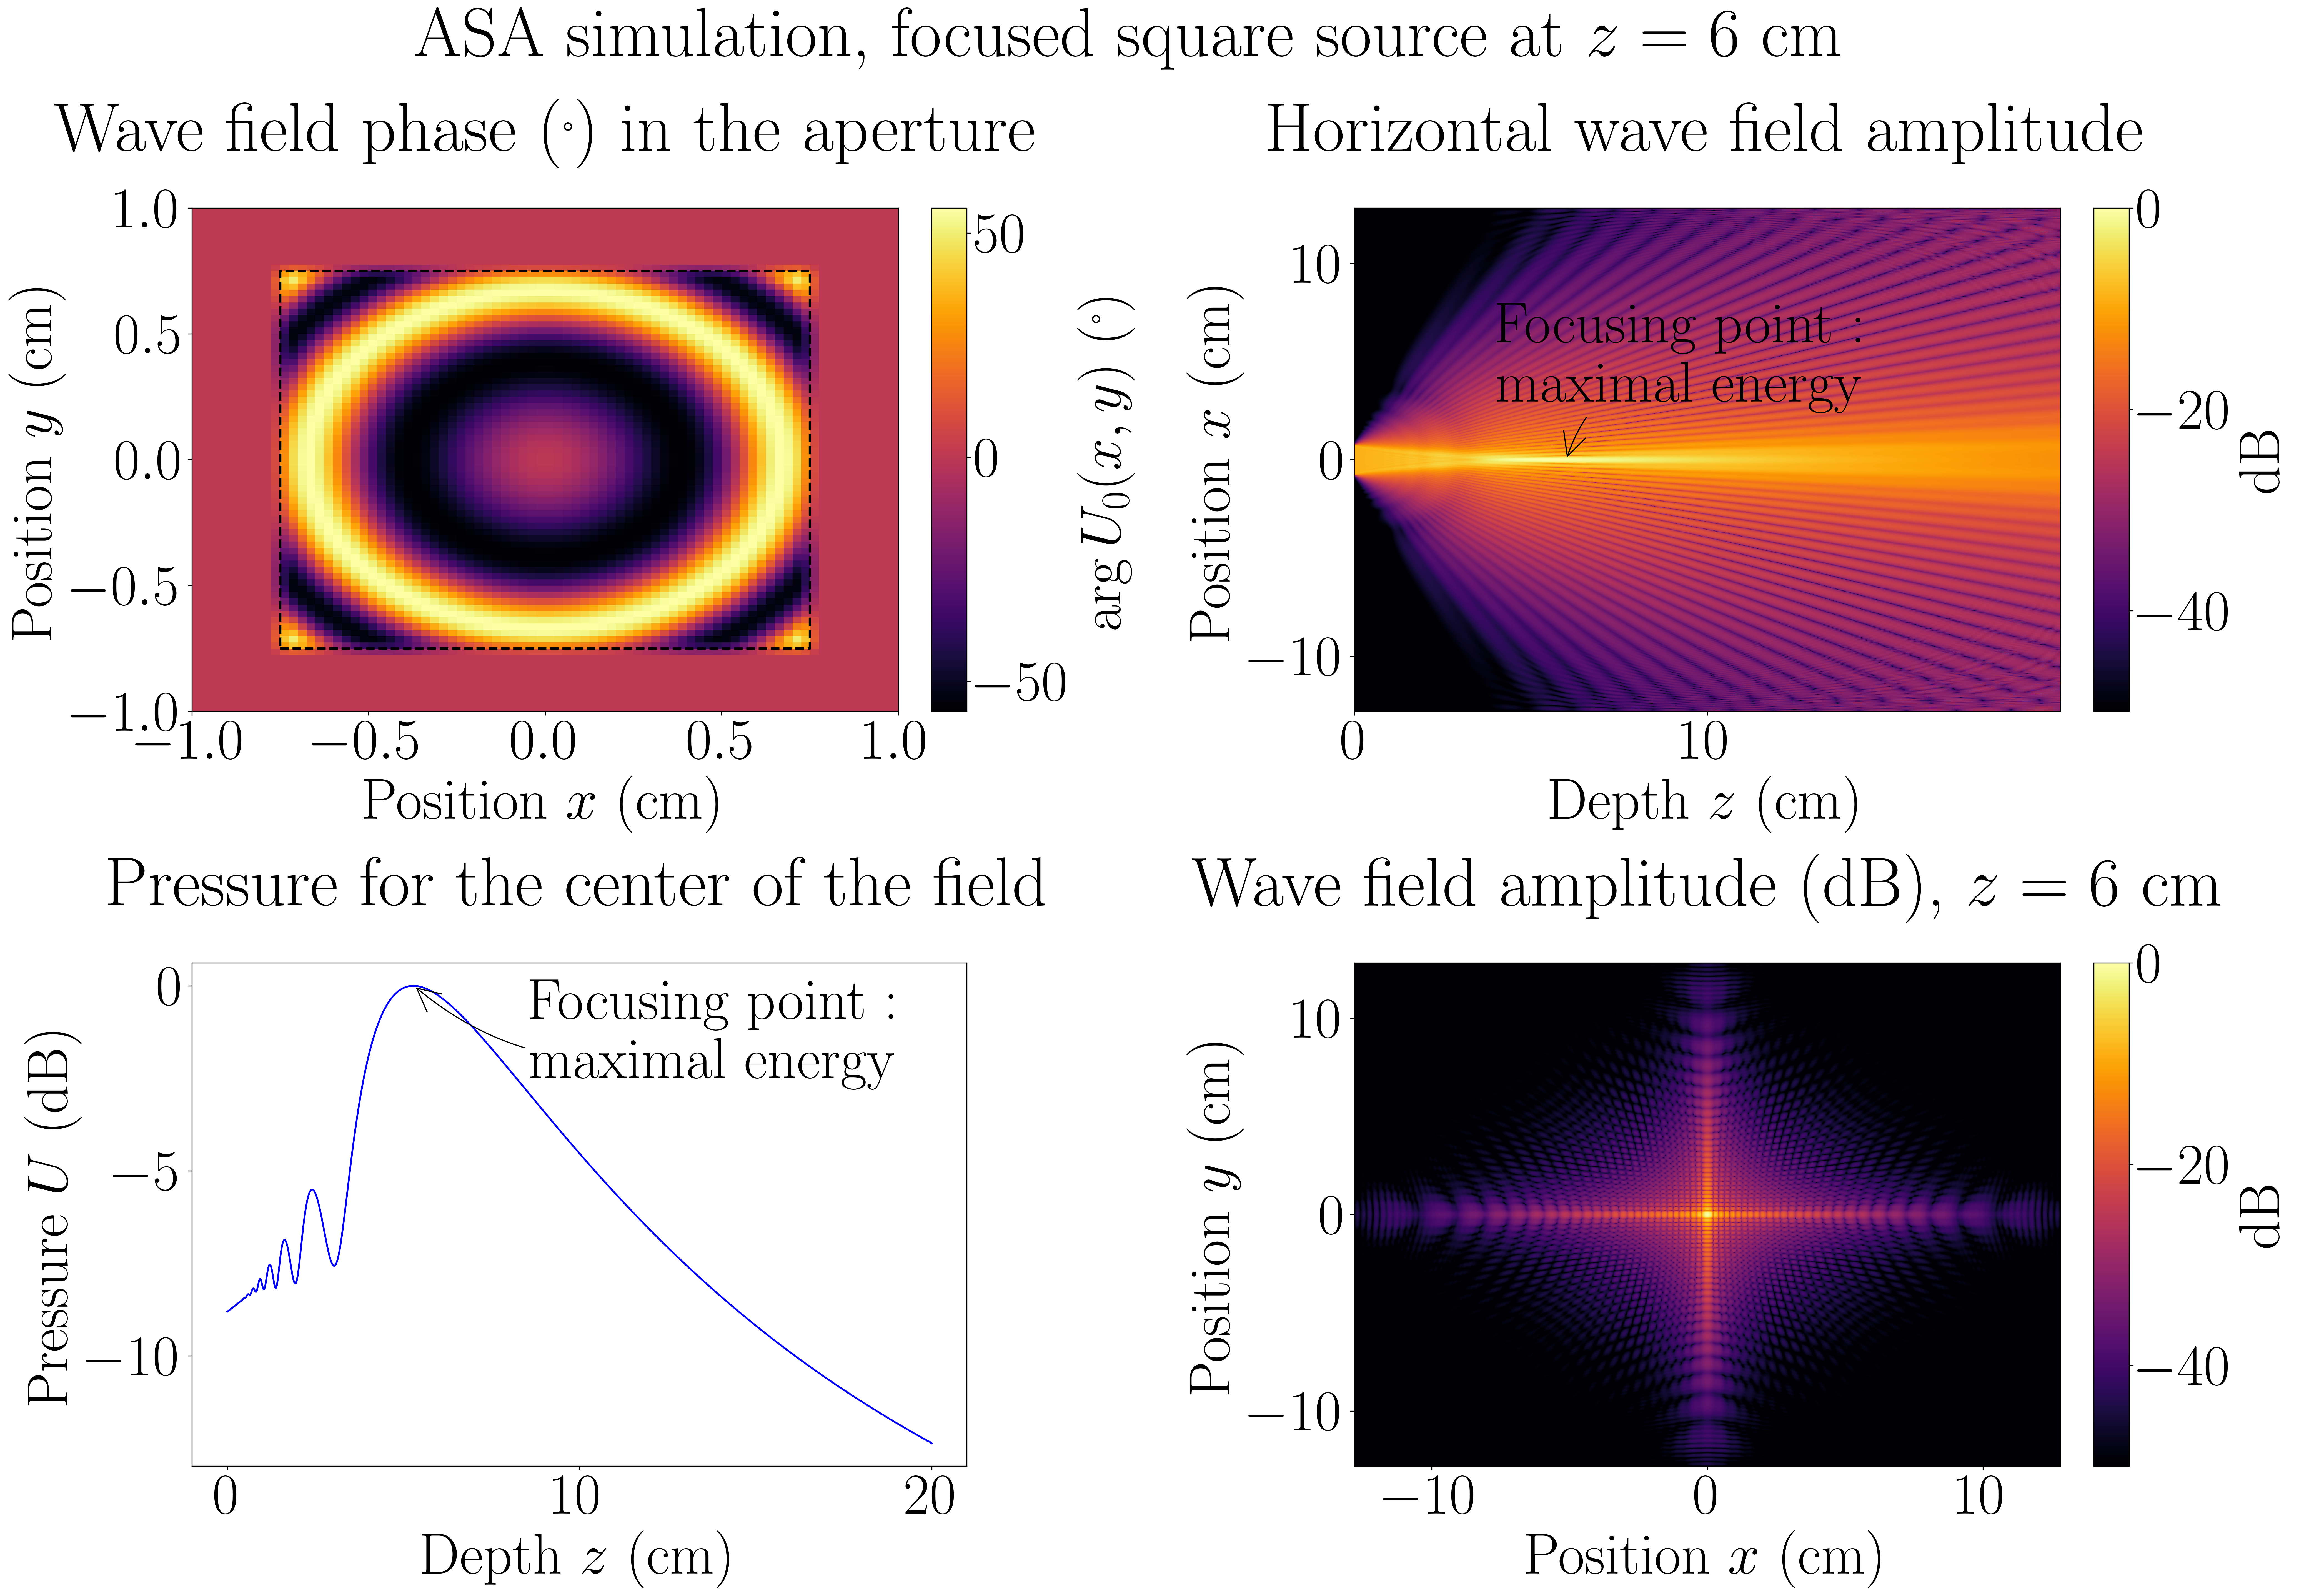
\includegraphics[scale=0.12]{square/all_smoothed_focused.png}
			\centering
			\caption{ASA simulation for a focused square source}
		\end{figure}
	\end{column}
	\begin{column}{0.4\textwidth}
	\begin{itemize}
		\item \textcolor{red}{\textbf{Steered source}} : constant phase over circles (same distance to the focusing point $\implies$ same delay)
		\item All the energy is focused in one point\dots
		\item But this point is not really at $6~\si{\centi\meter}$
		\item Influence of the $\dfrac{1}{r}$ factor!
		\item Near the focusing point, we have the same pattern for the wave field amplitude as in the far field (here $\dfrac{\sin x}{x}$)
	\end{itemize}
		
	\end{column}
\end{columns}
	
	
	
	
	
	\end{frame}
	\section{Array pattern}
		\begin{frame}{Table of contents}
		\tableofcontents
	\end{frame}
	\subsection{Grating lobes}
	\begin{frame}
	\frametitle{Grating lobes}


\begin{columns}
	\begin{column}{0.6\textwidth}
		\begin{itemize}
		\item We consider a ULA with $M=24$ sensors
		\item Array pattern for different element spacings $d=\dfrac{\lambda}{4},\dfrac{\lambda}{2},\lambda$ and $2\lambda$
	\end{itemize}
		\begin{figure}[h!]
			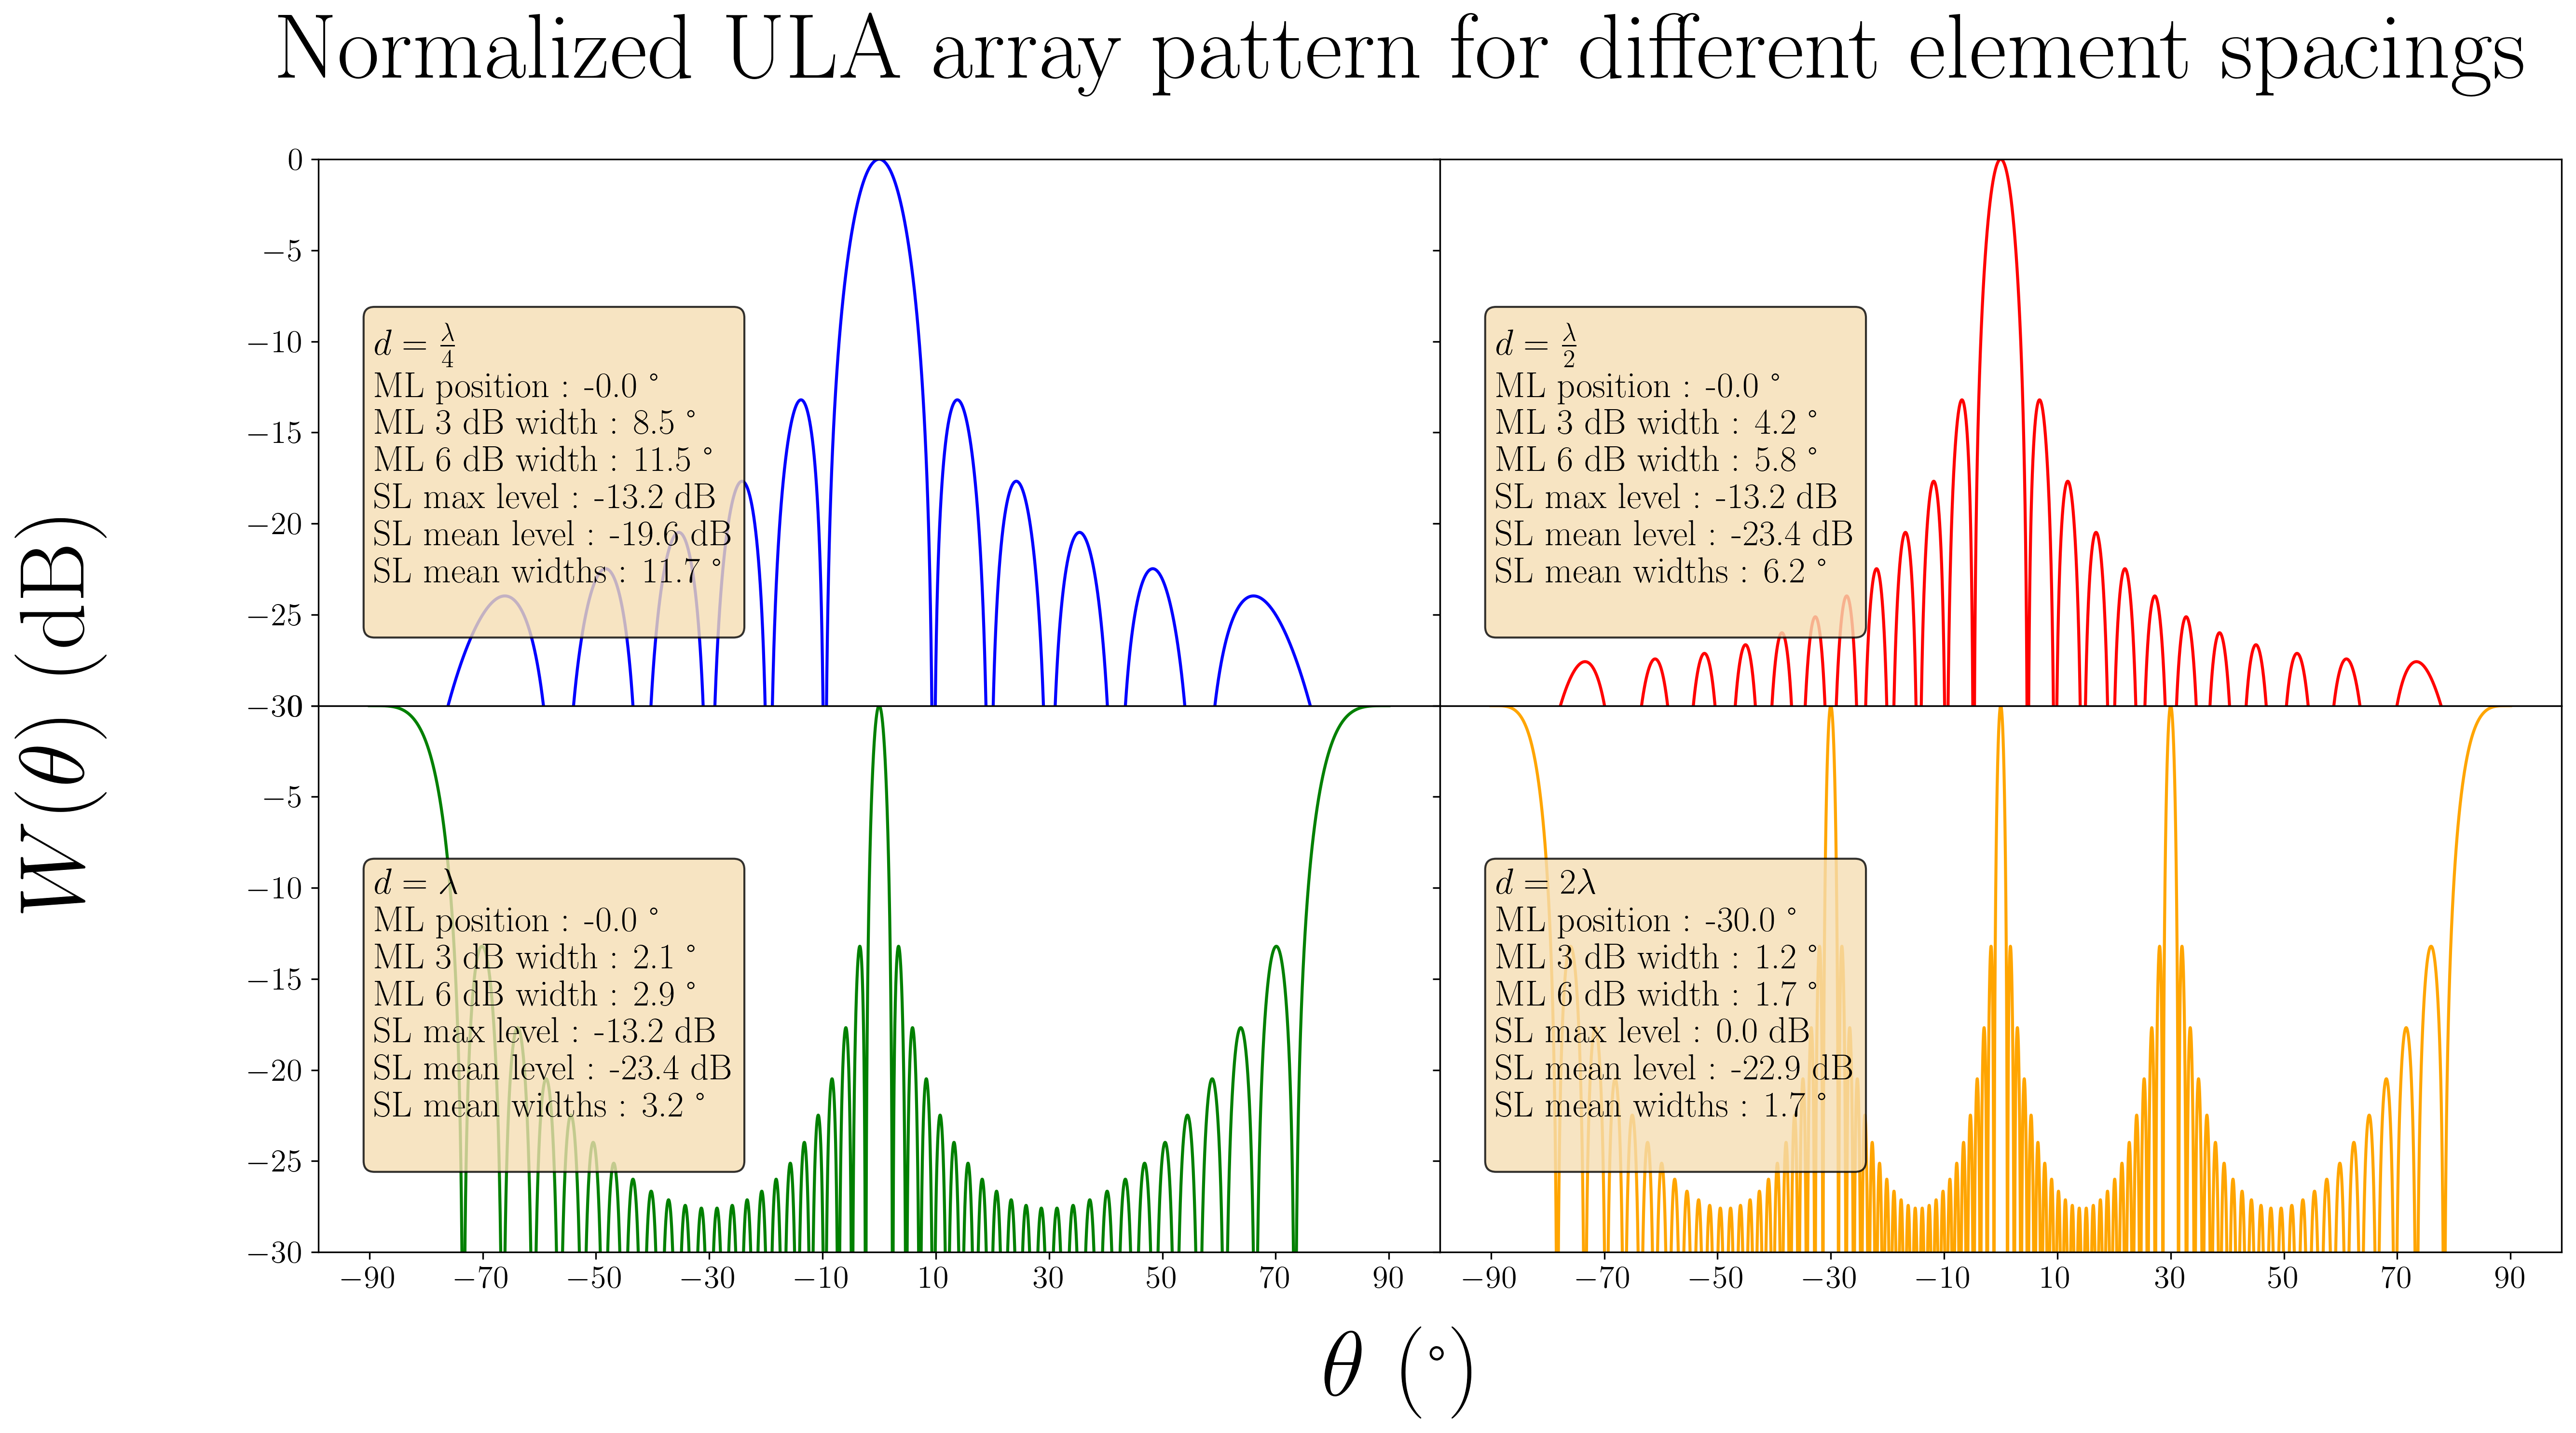
\includegraphics[scale=0.2]{ula_patterns_deg.png}
			\vspace{-5pt}
			\caption{Array patterns for multiple element spacings}
			\centering
		\end{figure}
	\vspace{-10pt}
	Equivalent results when plotting $W(k_x)$, the plot is just compressed because $k_x=\dfrac{2\pi}{\lambda}\sin\theta$ is not the identity function. 
	\end{column}
	\begin{column}{0.35\textwidth}
		\vspace{-30pt}
			\begin{figure}[h!]
			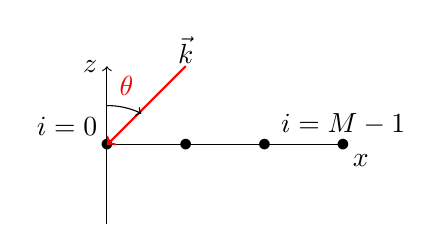
\begin{tikzpicture}
				\draw (1,0)--(4,0);
				\draw (4,0) node [below right] {$x$};
				\draw (1,0) node [above left] {$i=0$};
				\draw (4,0) node [above] {$i=M-1$};
				\draw [->](1,-1)--(1,1);
				\draw (1,1) node [ left] {$z$};
				
				\foreach \i in {1,...,4}{
					\draw (\i,0) node {$\bullet$};
				}
			
			\draw [<-,red,thick] (1,0)--(2,1);
			\draw (2,1.2) node {$\vec{k}$};
			
			\draw[black, ->] (1,0.5) arc (90:64:1);
			\draw (1.25,0.75) node {\textcolor{red}{$\theta$}};
			
			\end{tikzpicture}
			\centering
			\caption{ULA geometry}
		\end{figure}
	
		\begin{itemize}
			\item ML width $\searrow$ with $d$
			\item SL width $\searrow$ with $d$
			\item SL mean level $\searrow$ with $d$ ($-3~\si{\decibel}\Longleftrightarrow$ divided by 2)
			\item For $d=\dfrac{\lambda}{4}$ and  $d=\dfrac{\lambda}{2}$ : \textcolor{red}{\textbf{no grating lobes but larger SL}} for $d=\dfrac{\lambda}{4}$
			\item $d=\lambda$ and $d=2\lambda$ : \textcolor{red}{\textbf{grating lobes}} because we don't verify the \textcolor{red}{\textbf{ULA sampling criterion}} + aliasing in the reconstructed signal
			\item \textcolor{red}{\textbf{More grating lobes}} for $d=2\lambda$ : the period of the function is reduced $\implies$ more grating lobes in the window $\sin\theta\in[-1,1]$
		\end{itemize}
	\end{column}
\end{columns}

\end{frame}
	\subsection{Element weighting and element spacing}
	\begin{frame}
		\frametitle{Element weighting and element spacing : \textsc{KAISER} window}
		\begin{itemize}
			\item We apply a \textsc{KAISER} window $\implies$ new weights : $\vec{w}_{\textsc{KAISER}}=\mathcal{K}\cdot\vec{w}$
		\end{itemize}
	\begin{columns}
	
			\begin{column}{0.5\textwidth}
				\vspace{-15pt}
			\begin{figure}
				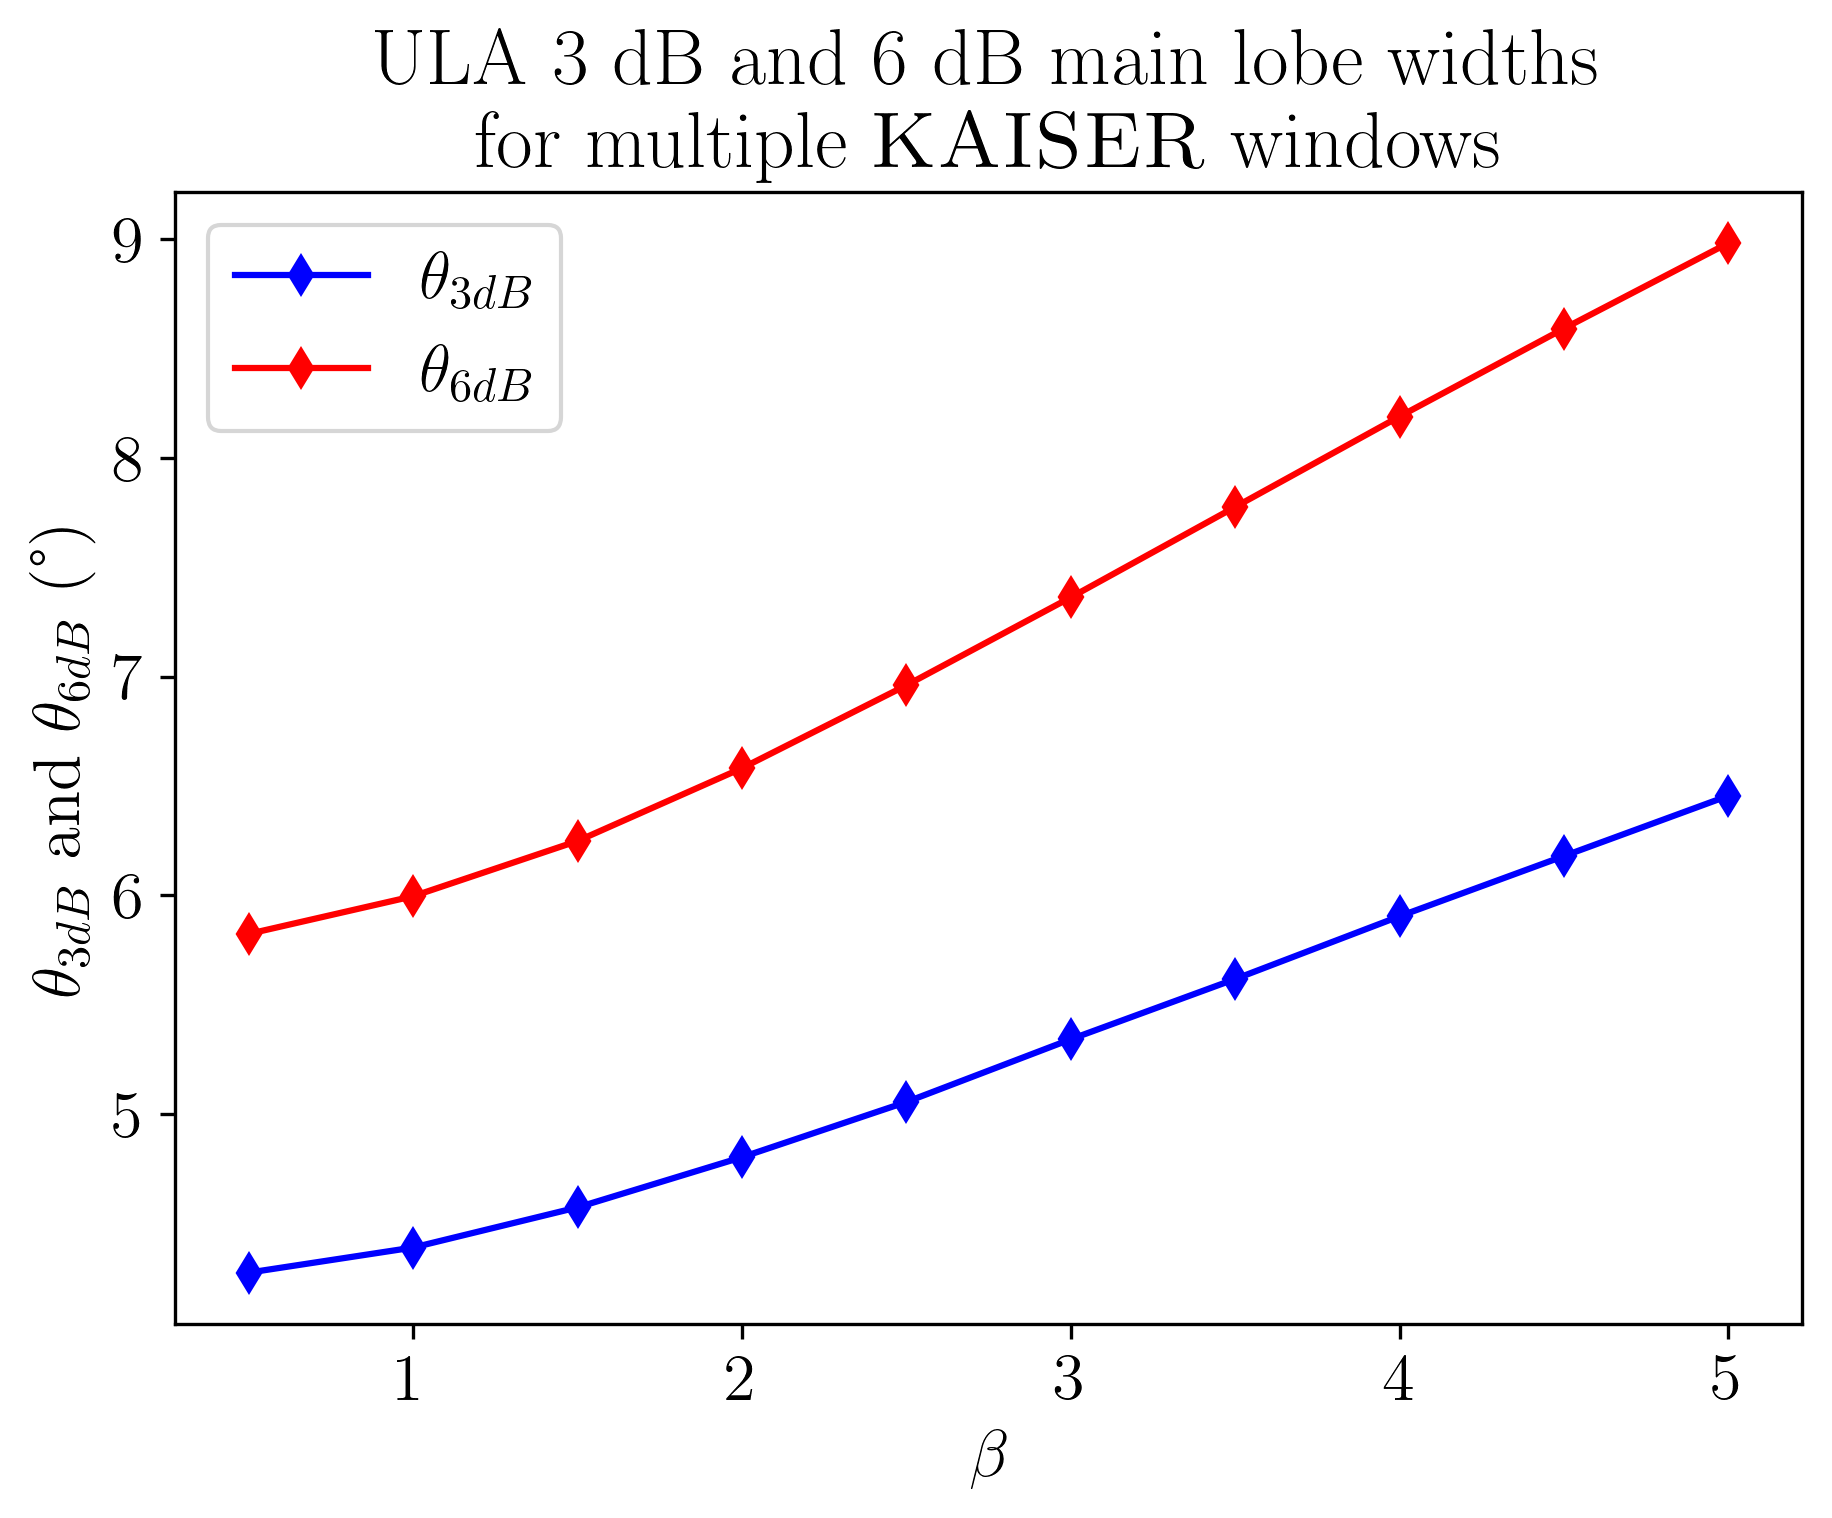
\includegraphics[scale=0.3]{ula_kaiser_lobe_widths.png}
				\centering
				\vspace{-5pt}
				\caption{Influence of the \textsc{KAISER} window on the main lobe width}
			\end{figure}
		\vspace{-20pt}
		\begin{figure}
			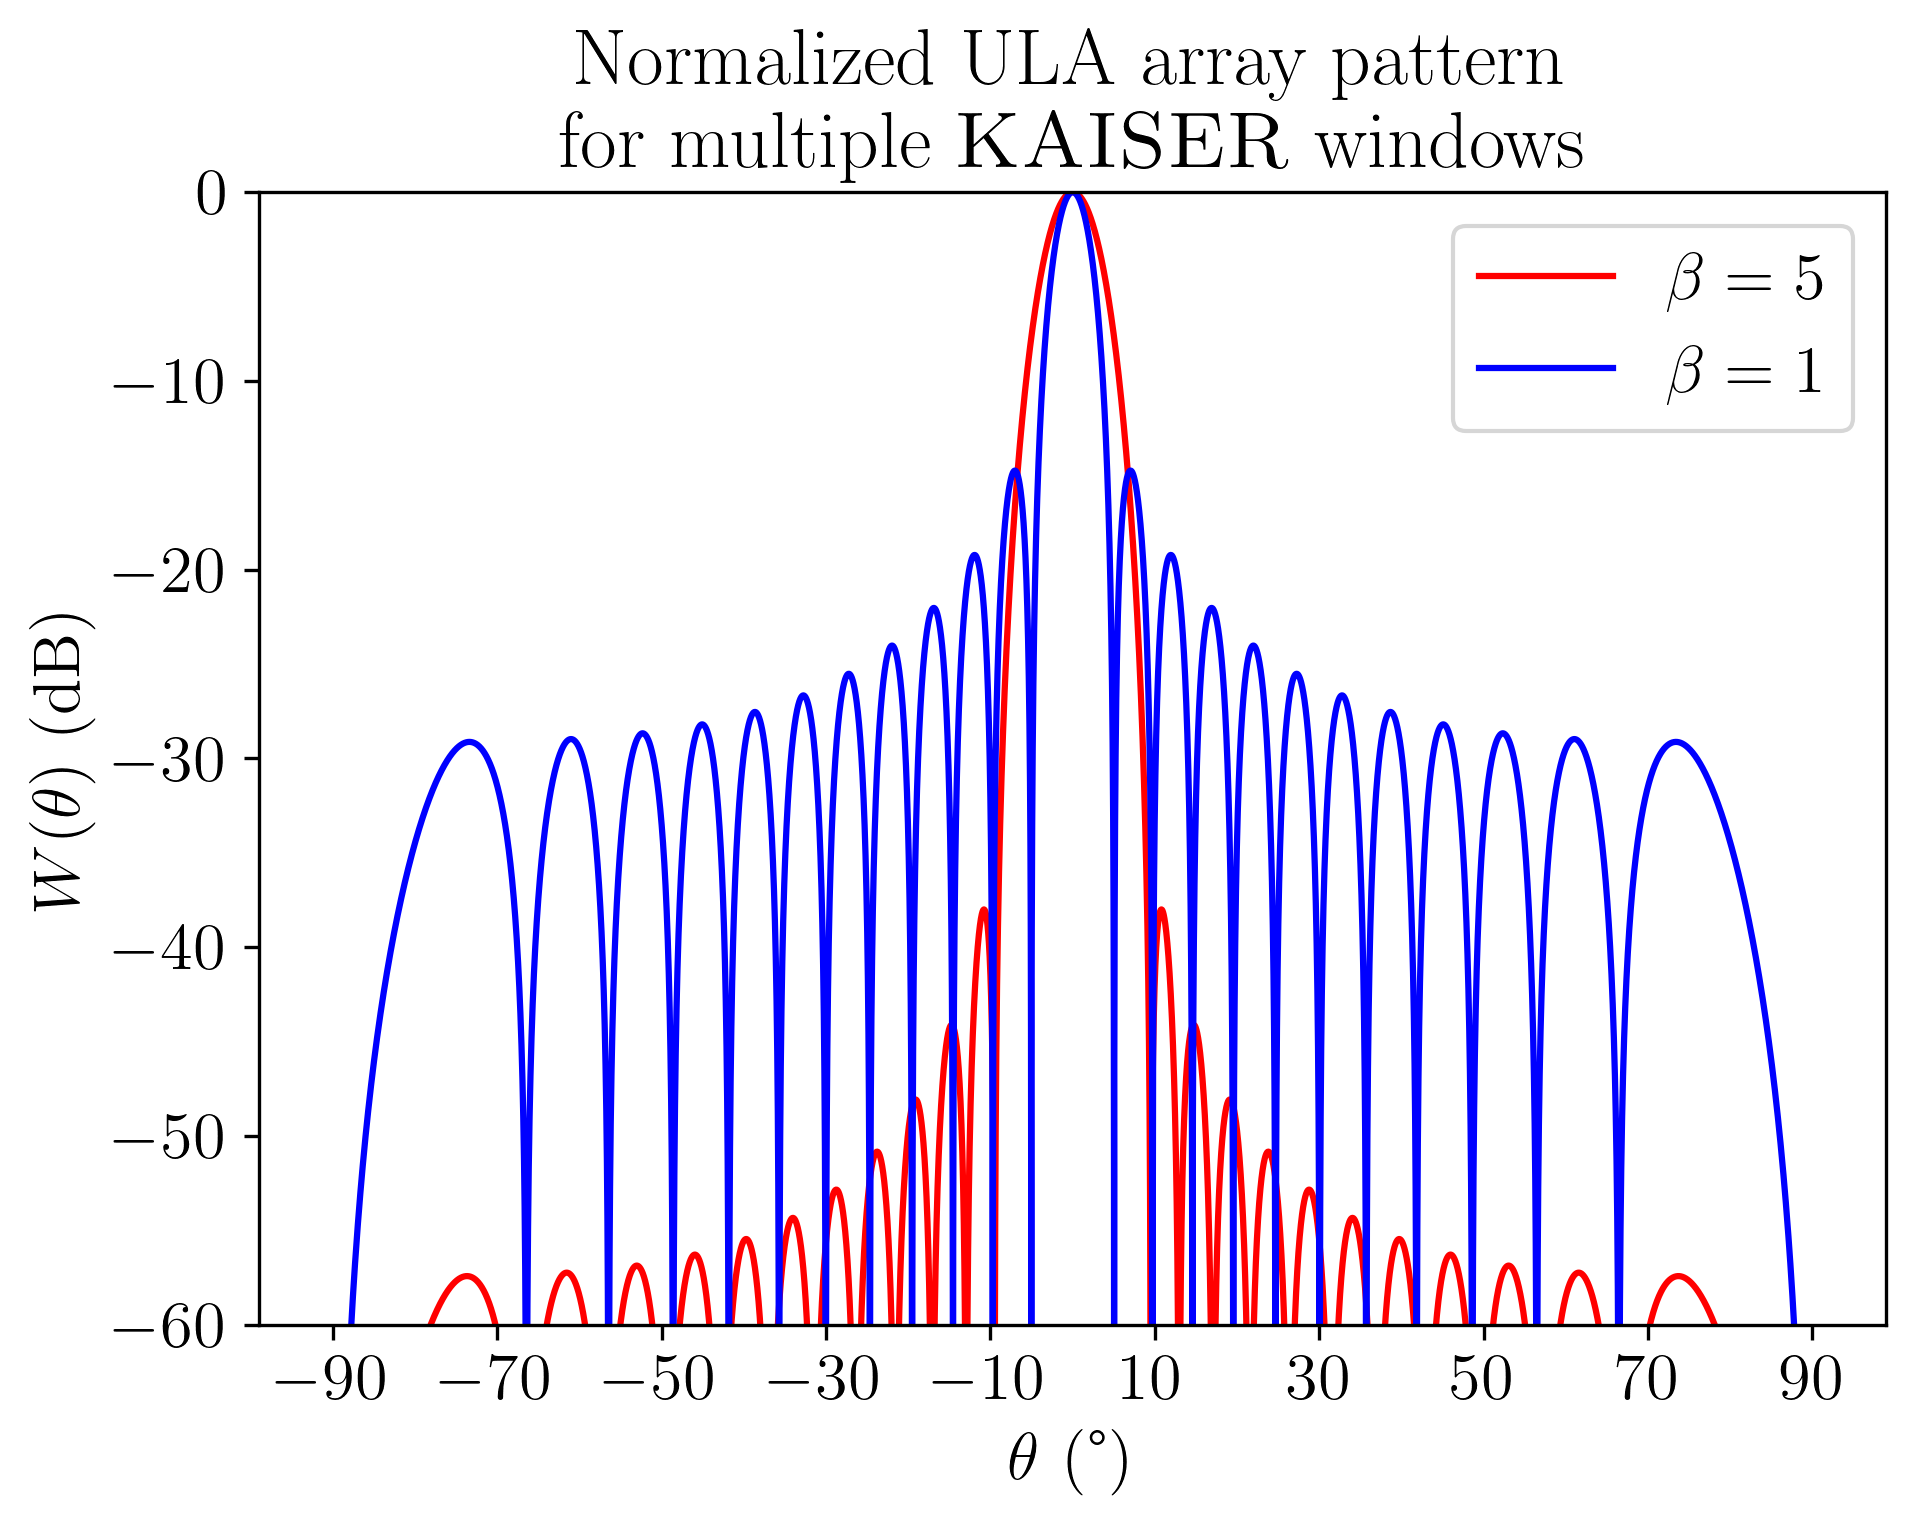
\includegraphics[scale=0.3]{ula_kaiser_comp.png}
			\centering
			\vspace{-5pt}
			\caption{Influence of the \textsc{KAISER} window on the array pattern}
		\end{figure}
			
		\end{column}
	
		\begin{column}{0.5\textwidth}
				\vspace{-15pt}
			\begin{figure}
			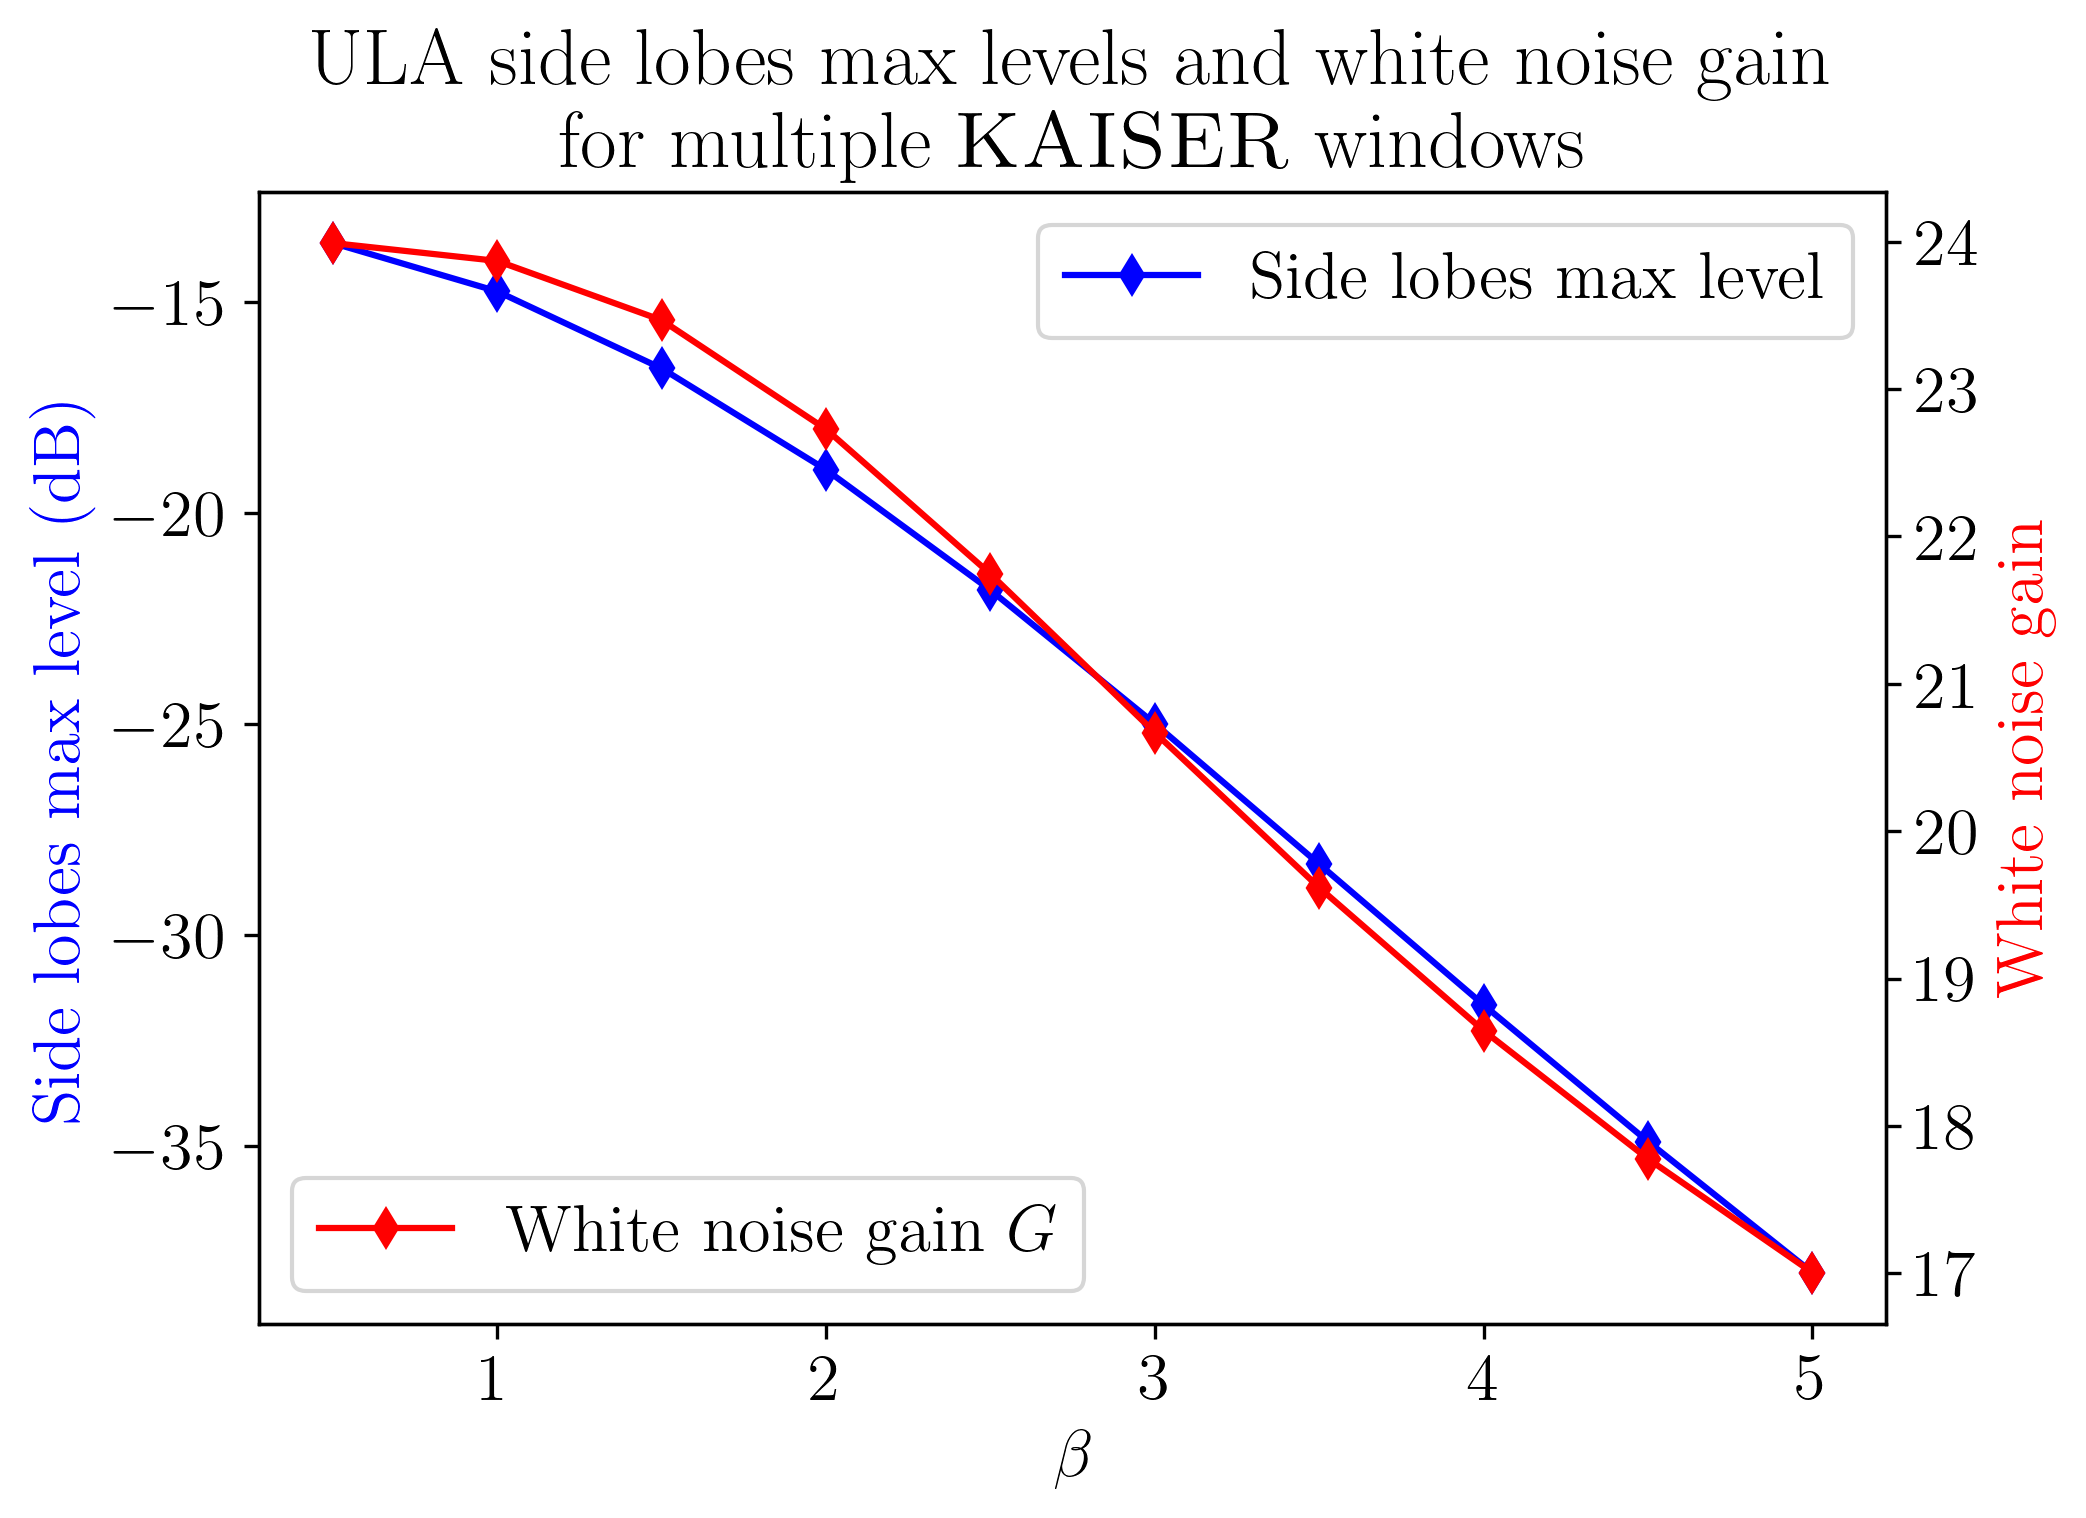
\includegraphics[scale=0.3]{ula_kaiser_SL_max_white_noise_gain.png}
			\centering
			\vspace{-5pt}
			\caption{Influence of the \textsc{KAISER} window on the  side lobes max level and white noise gain}
		\end{figure}
		

\begin{itemize}
	\item Larger SL but with lower levels
	\item Larger ML
	\item Same aperture size
	\item \textcolor{red}{\textbf{Spatial resolution decreases}!}
	\item \textcolor{red}{\textbf{Lower white noise gain}} $\implies$ we decrease the noise level\dots
	\item \textcolor{red}{\textbf{Trade-off}}
	\item Other windows : \textsc{HANNING}, \textsc{CHEBYSHEV}\dots 
\end{itemize}
	\end{column}
\end{columns}

	\end{frame}


\begin{frame}
	\frametitle{Array from \cite{Nonuniformly_spaced_linear} }
	\begin{columns}
	
	\begin{column}{0.5\textwidth}
		\vspace{-15pt}
		\begin{figure}
			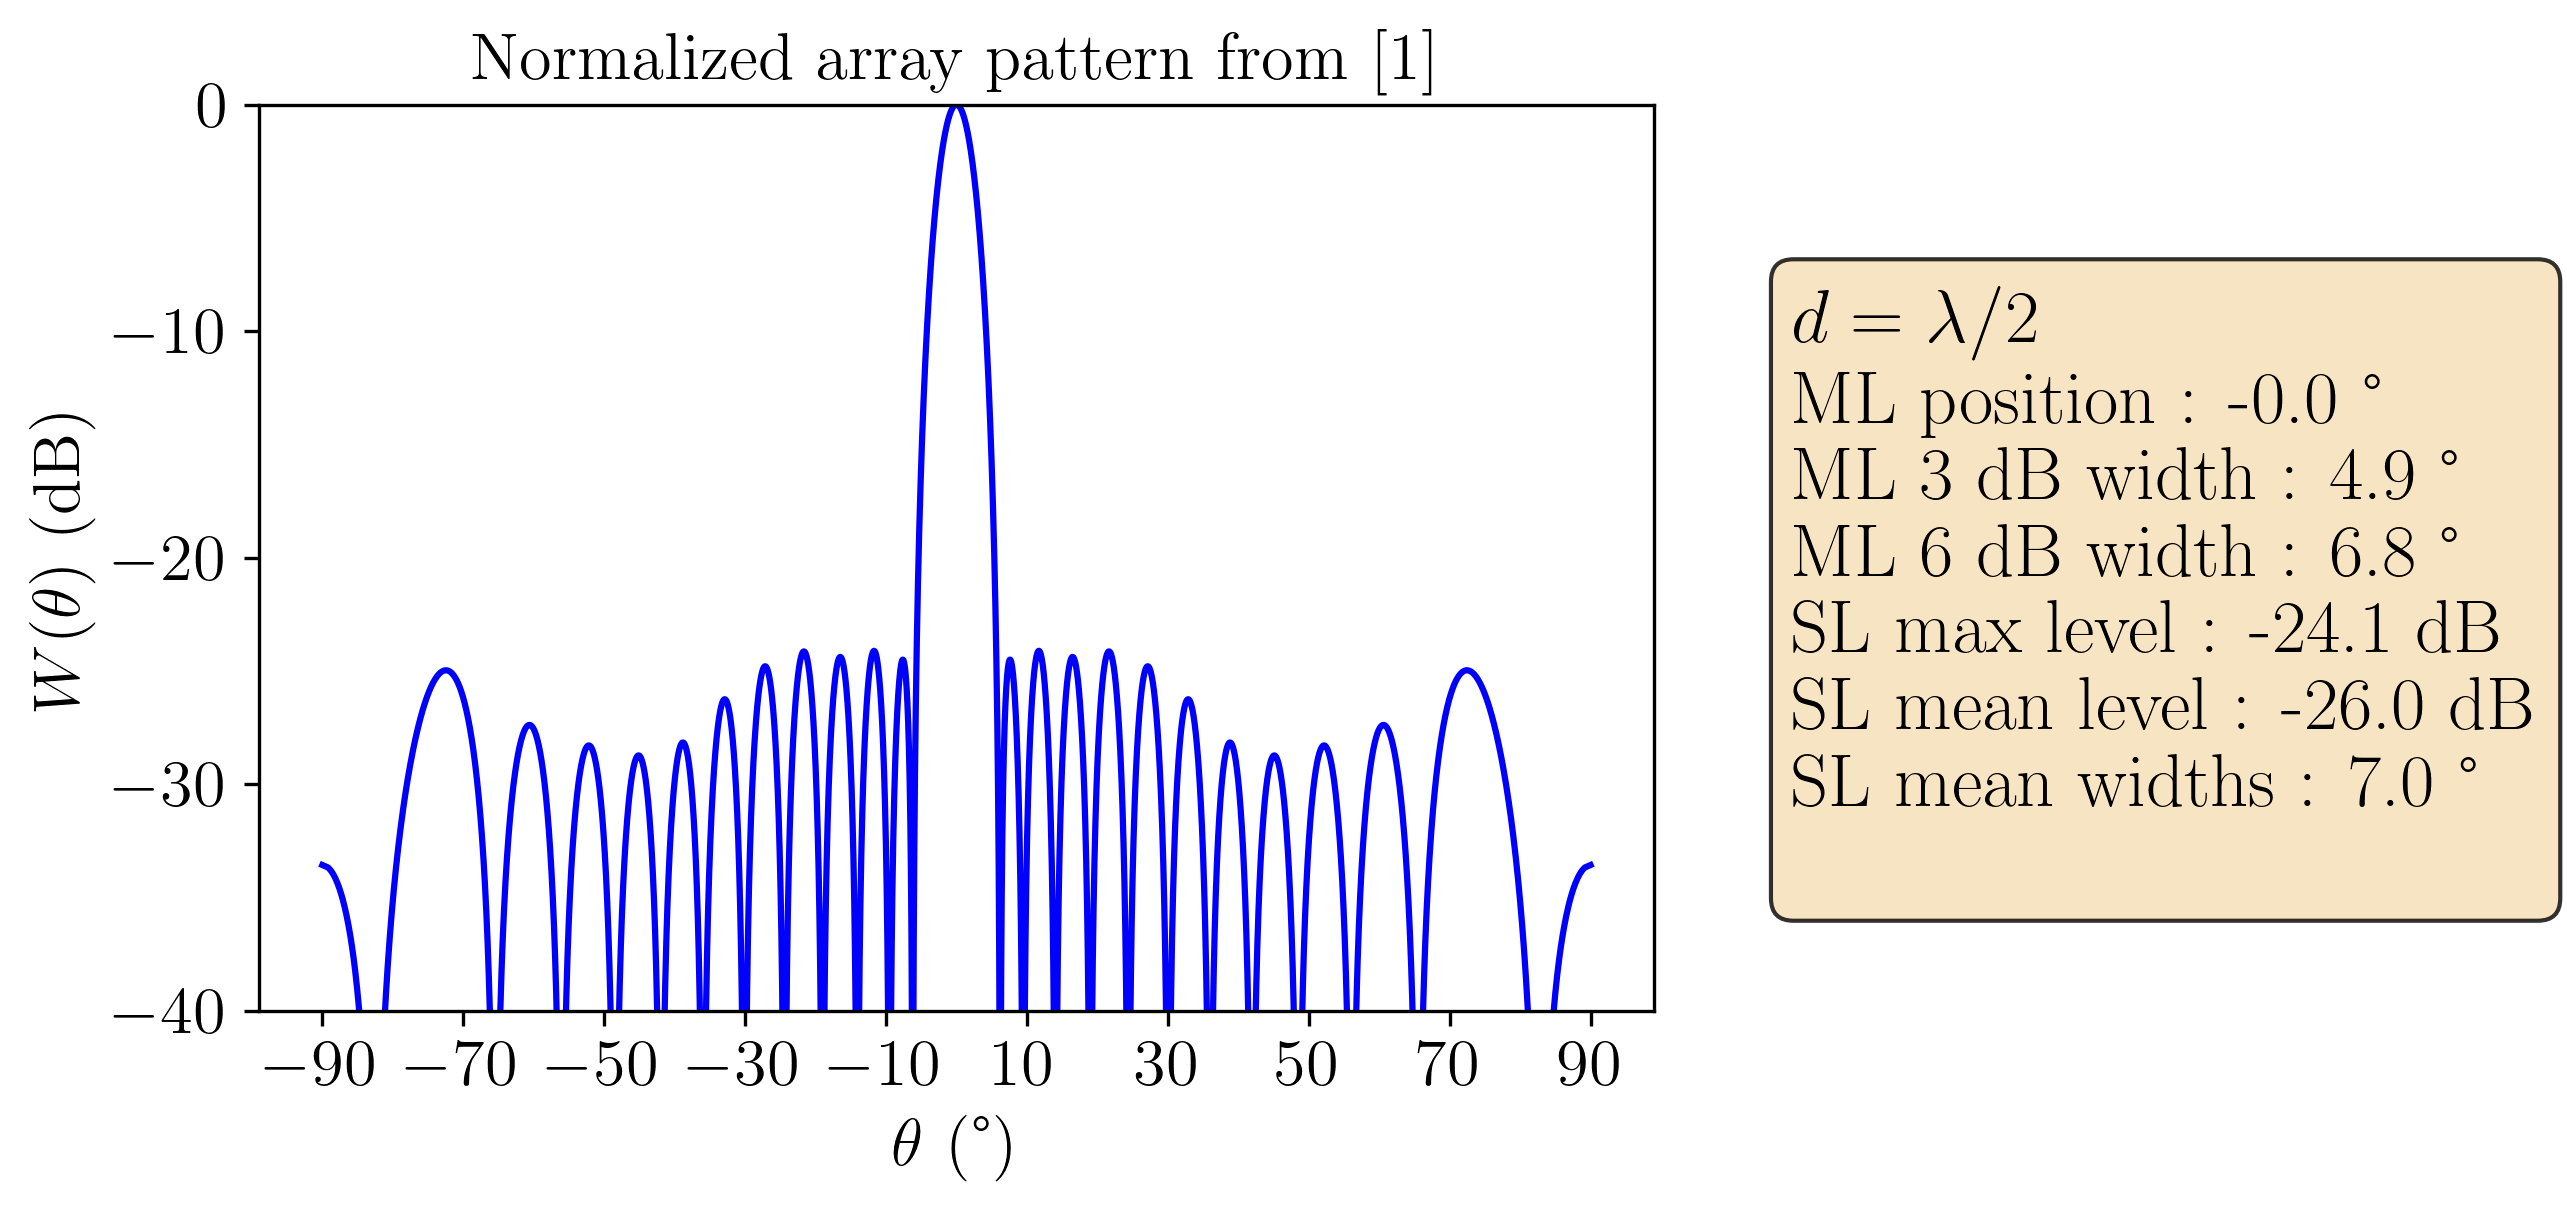
\includegraphics[scale=0.35]{ElPos_array_pattern.png}
			\centering
				\vspace{-15pt}
			\caption{Array pattern from \cite{Nonuniformly_spaced_linear}}
		\end{figure}
	
		
	\end{column}
	
	\begin{column}{0.5\textwidth}
		\vspace{-15pt}
		\begin{figure}
			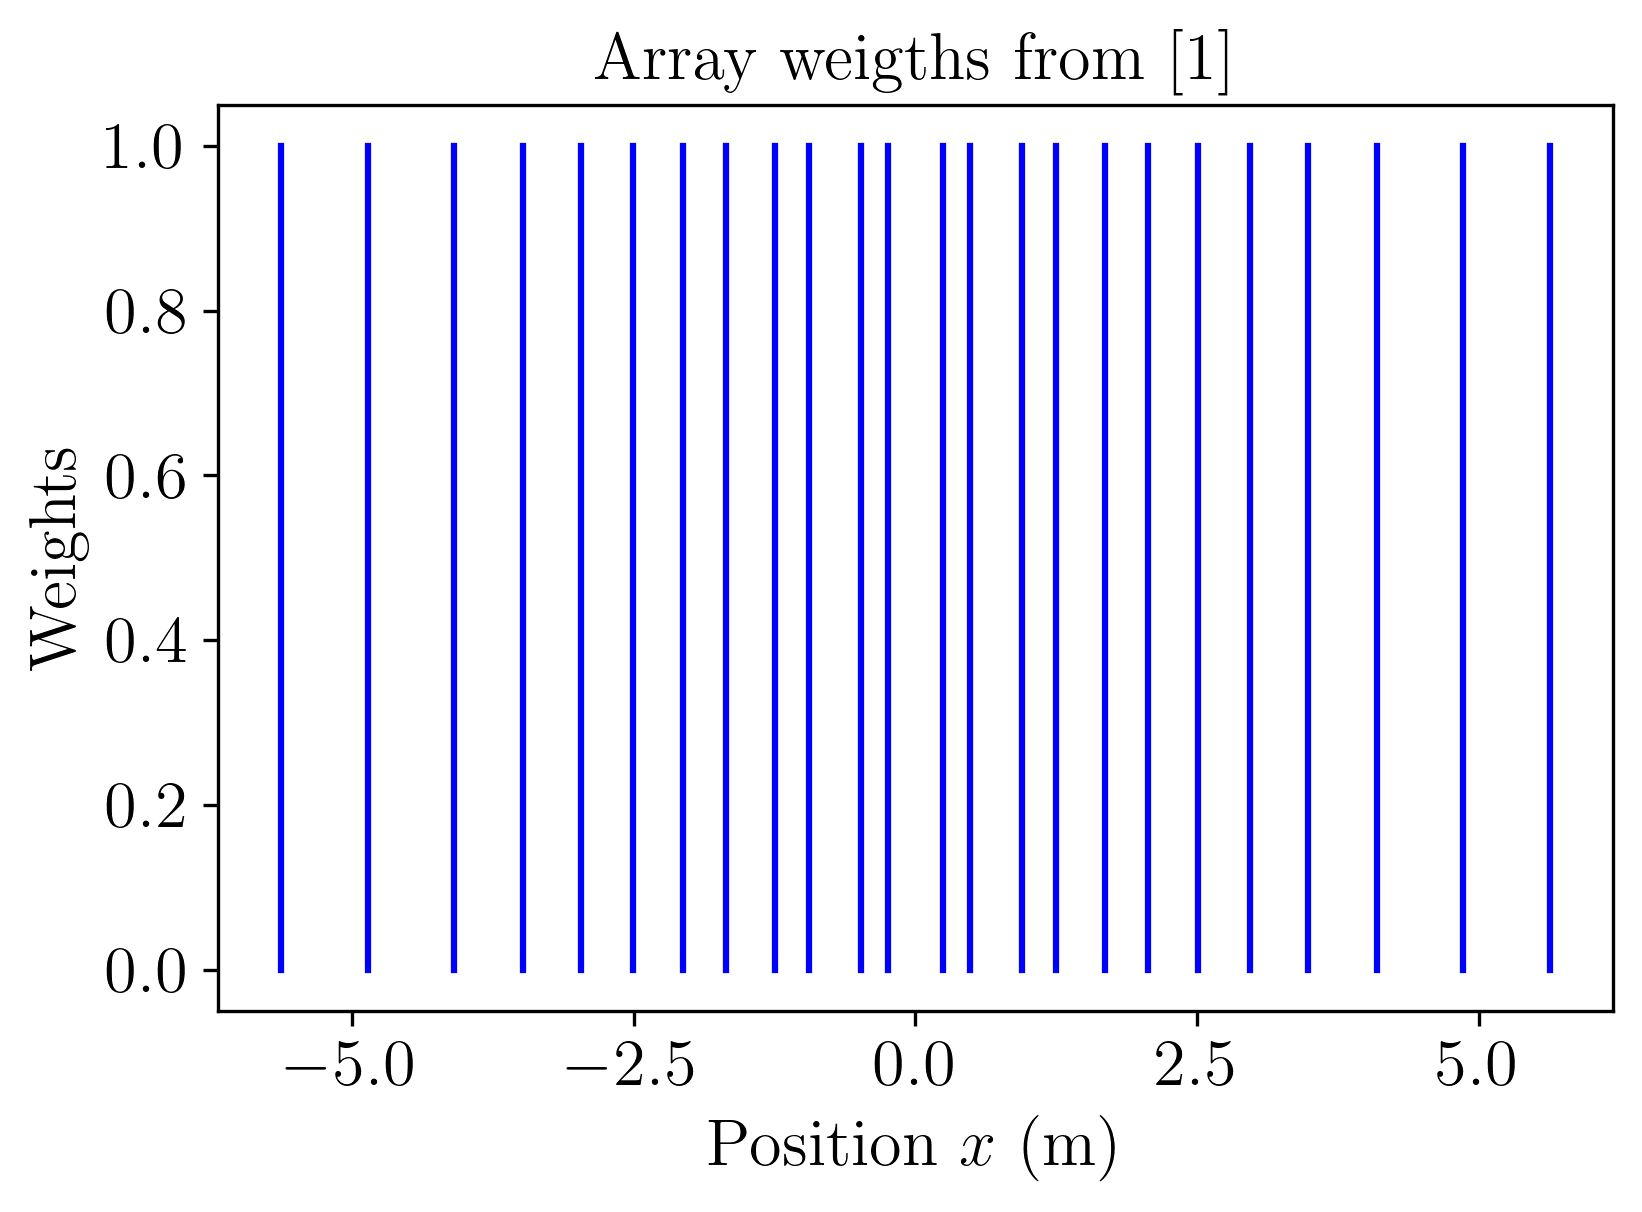
\includegraphics[scale=0.35]{ElPos_array_pattern_weights.png}
			\centering	
			\vspace{-5pt}
			\caption{Array weights from \cite{Nonuniformly_spaced_linear}}
		\end{figure}
		
	\end{column}
\end{columns}
\vspace{-5pt}
We compare multiple arrays with same : number of sensors $M=24$, same element spacing $d=\dfrac{\lambda}{2}$ $\implies$ same size
\vspace{-5pt}
	\begin{table}
	\begin{tabular}{cccccccc}
	\hline
	\multirow{2}{*}{Array}&\multicolumn{2}{c}{ML width \si{\degree}}&\multicolumn{3}{c}{SL}&Grating&White 
	\\
	&$3~\si{\decibel}$&$6~\si{\decibel}$&Mean width ($\si{\degree}$)&Mean level (\si{\decibel})&Max level (\si{\decibel})&lobes&noise gain
	\\
	\hline
	\hline
	Standard ULA&4.2&11.5&11.7&-19.6&-13.2&\textcolor{green}{\faCheck}&$24$
	\\
	ULA + \textsc{KAISER} ($\beta=1$)&4.4&6.0&6.1&-25.0&-14.7&\textcolor{green}{\faCheck}&$23.5$
	\\
	ULA + \textsc{KAISER} ($\beta=5$)&6.5&9.0&5.7&-52.0&-38.0&\textcolor{green}{\faCheck}&$17.0$
	\\
	Array from \cite{Nonuniformly_spaced_linear}&\textbf{4.9}&\textbf{6.8}&\textbf{7.0}&\textbf{-26.0}&\textbf{-24.1}&\textcolor{green}{\faCheck}&$24$
	\\
	\hline
	\end{tabular}
	\caption{Comparison of multiples arrays}
		\centering
\end{table}
\begin{itemize}
	\item Array from \cite{Nonuniformly_spaced_linear} : \textcolor{red}{\textbf{same white noise gain}} as a ULA but with \textcolor{red}{\textbf{lower narrower SL}} ($-6~\si{\decibel}$)
\end{itemize}
\end{frame}




\begin{frame}
	\frametitle{Steering}
	\begin{columns}
		
		\begin{column}{0.33\textwidth}
			\vspace{-15pt}
			\begin{figure}[h!]
				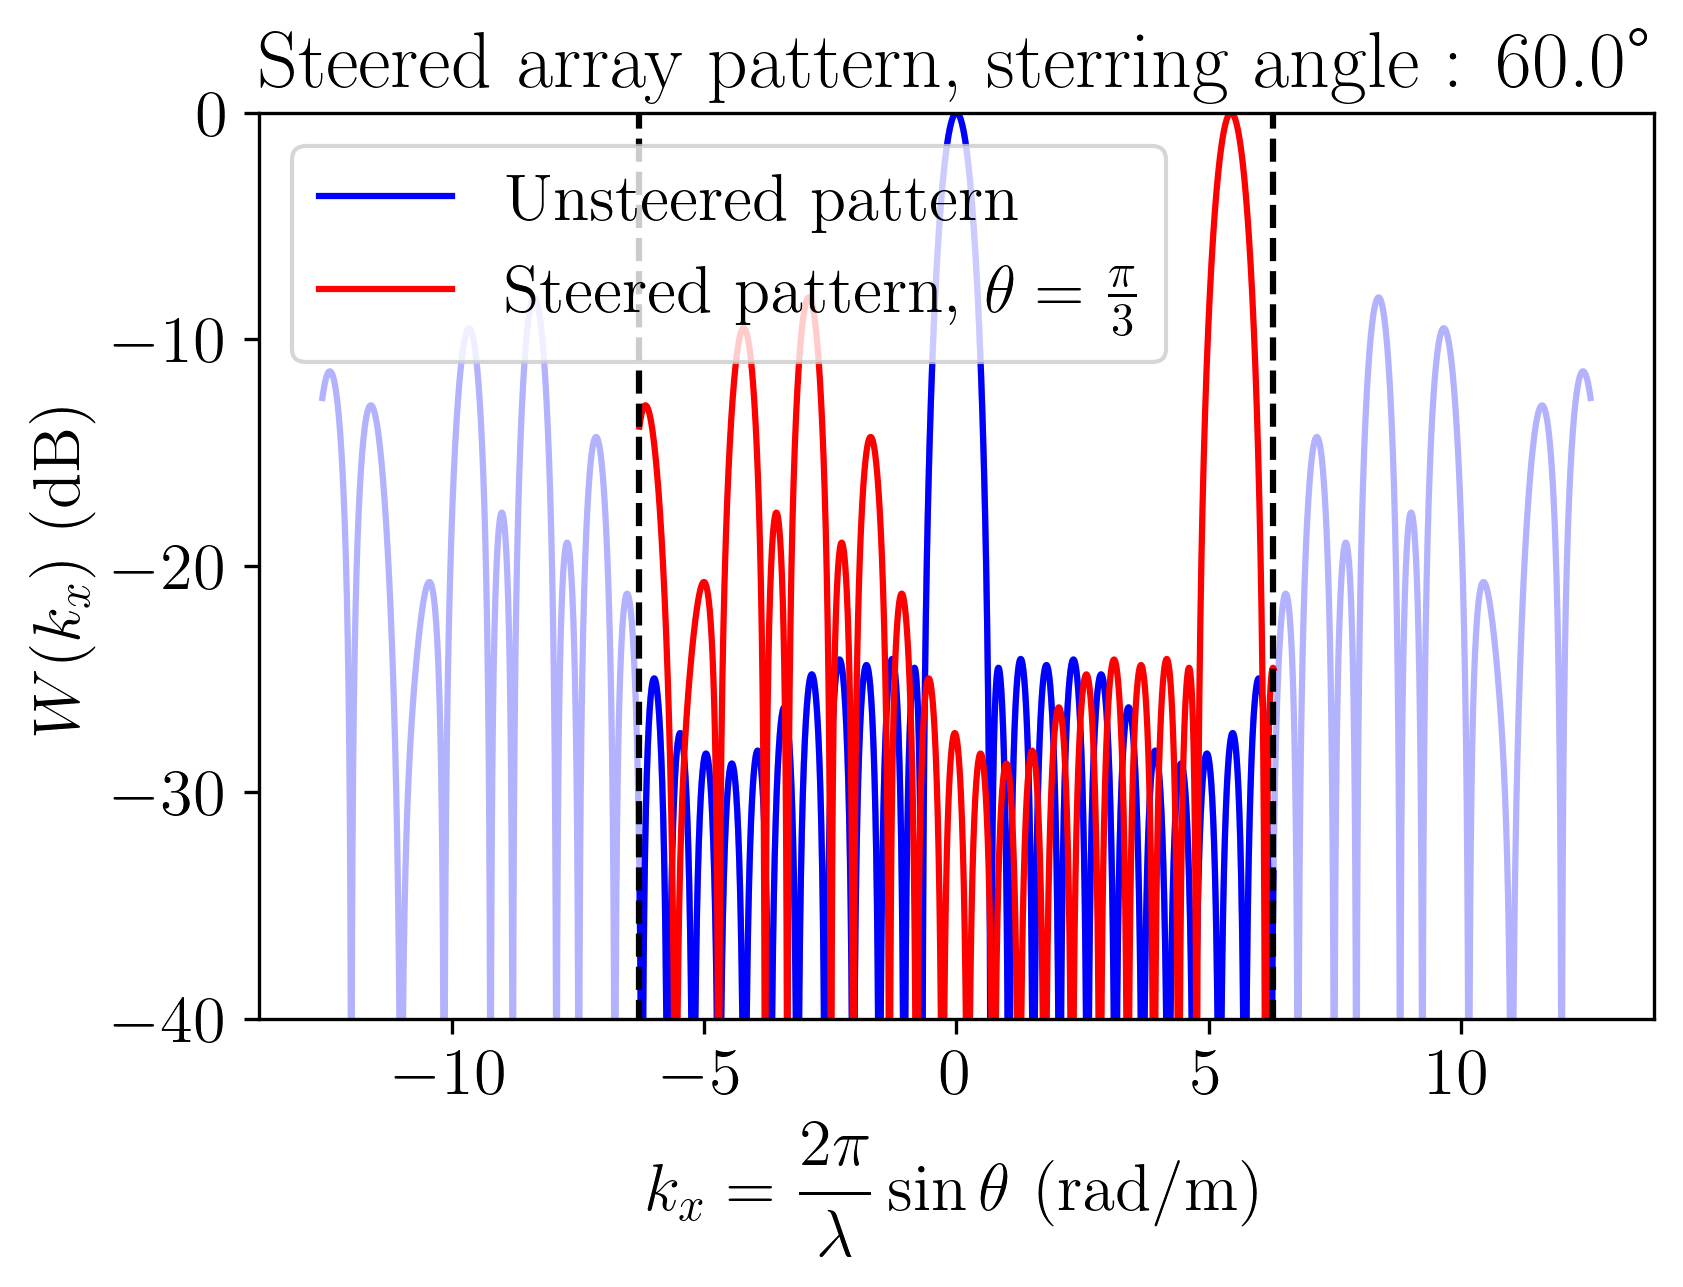
\includegraphics[scale=0.3]{/steered_array_pattern_elPos.png}
				\centering
				\caption{Steered array pattern \cite{Nonuniformly_spaced_linear}}
			\end{figure}
			
			
		\end{column}
		
		\begin{column}{0.33\textwidth}
			\vspace{-15pt}
			\begin{figure}[h!]
				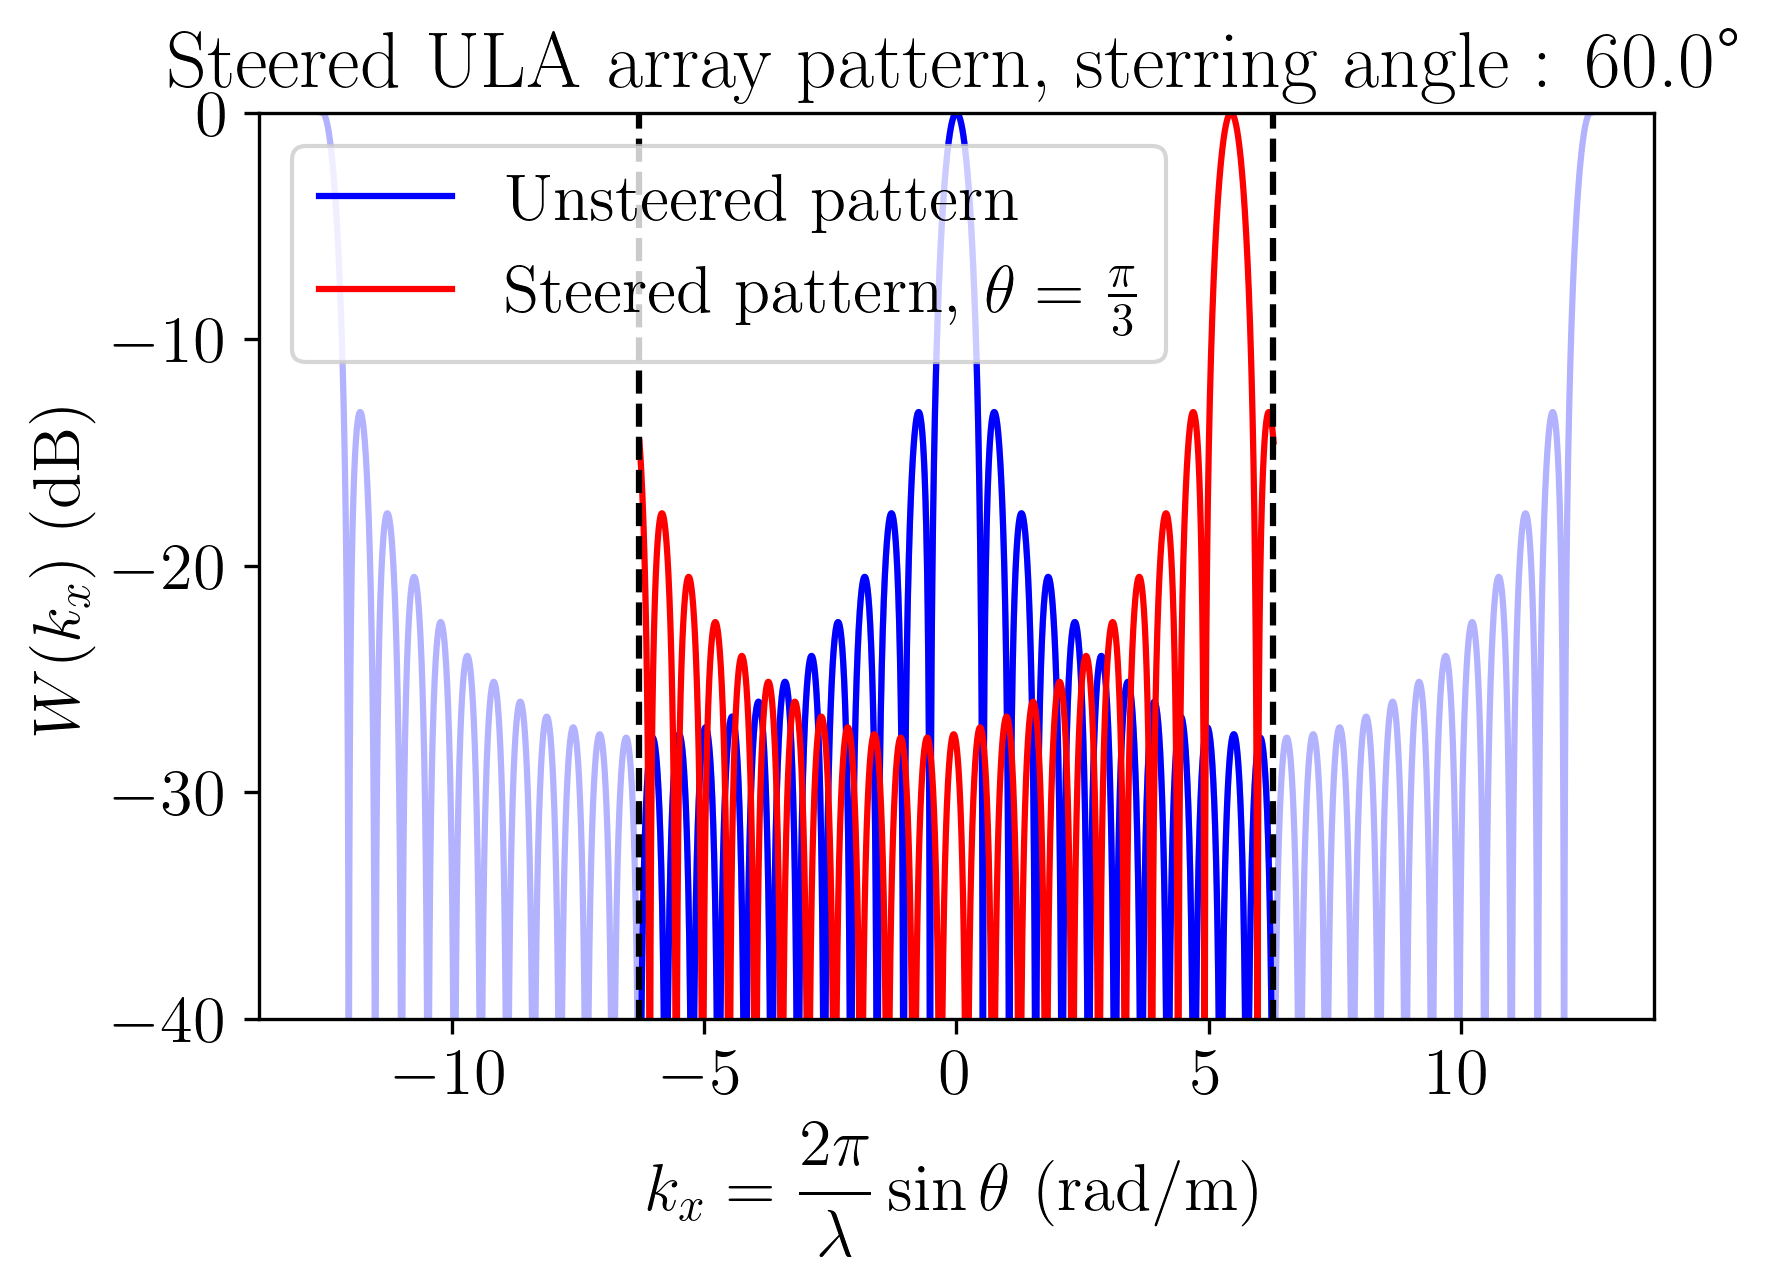
\includegraphics[scale=0.3]{steered_ULA_array_pattern.png}
				\centering
				\caption{Steered ULA  array pattern}
			\end{figure}
		\end{column}
	
		\begin{column}{0.33\textwidth}
		\vspace{-20pt}
		\begin{figure}[h!]
			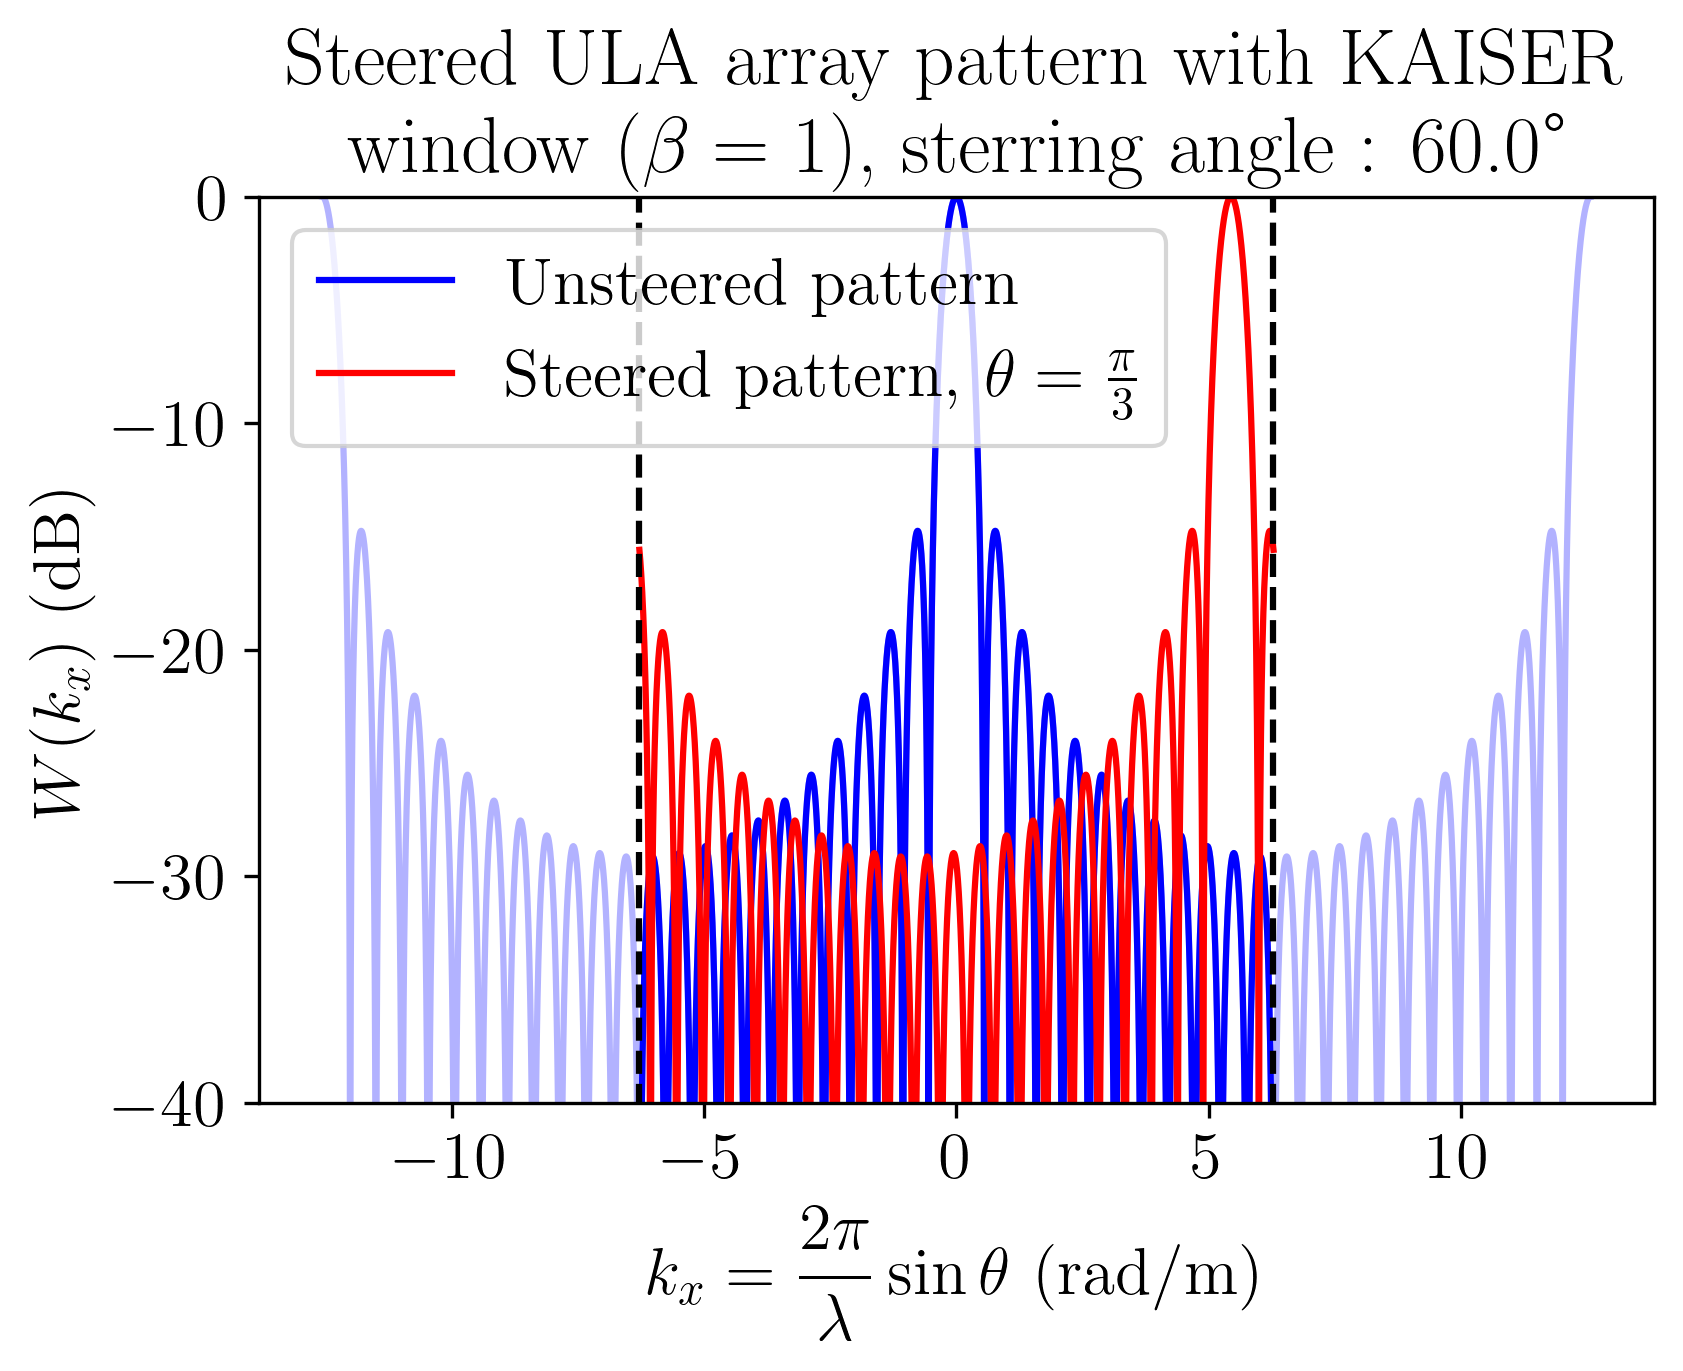
\includegraphics[scale=0.3]{steered_ULA_kaiser_array_pattern.png}
			\centering
			\caption{Steered ULA  array pattern with \textsc{KAISER} window ($\beta=1$)}
		\end{figure}
	\end{column}

	\end{columns}
\begin{itemize}
	\item Array from \cite{Nonuniformly_spaced_linear} :  very high side lobes $\implies$ \textcolor{red}{\textbf{grating lobes}}\dots 
    \item Why? Grating lobes are extremely close to the visible region! 
	\item Steered ULA and ULA with \textsc{KAISER} window arrays patterns are free form grating lobes!
	\item \textcolor{red}{\faHandPointRight} For very low sterring angles, the pattern might be free from grating lobes
\end{itemize}
\end{frame}



\begin{frame}
	\frametitle{Steering}
		\begin{columns}
		
		\begin{column}{0.5\textwidth}
			\vspace{-15pt}
			\begin{figure}
				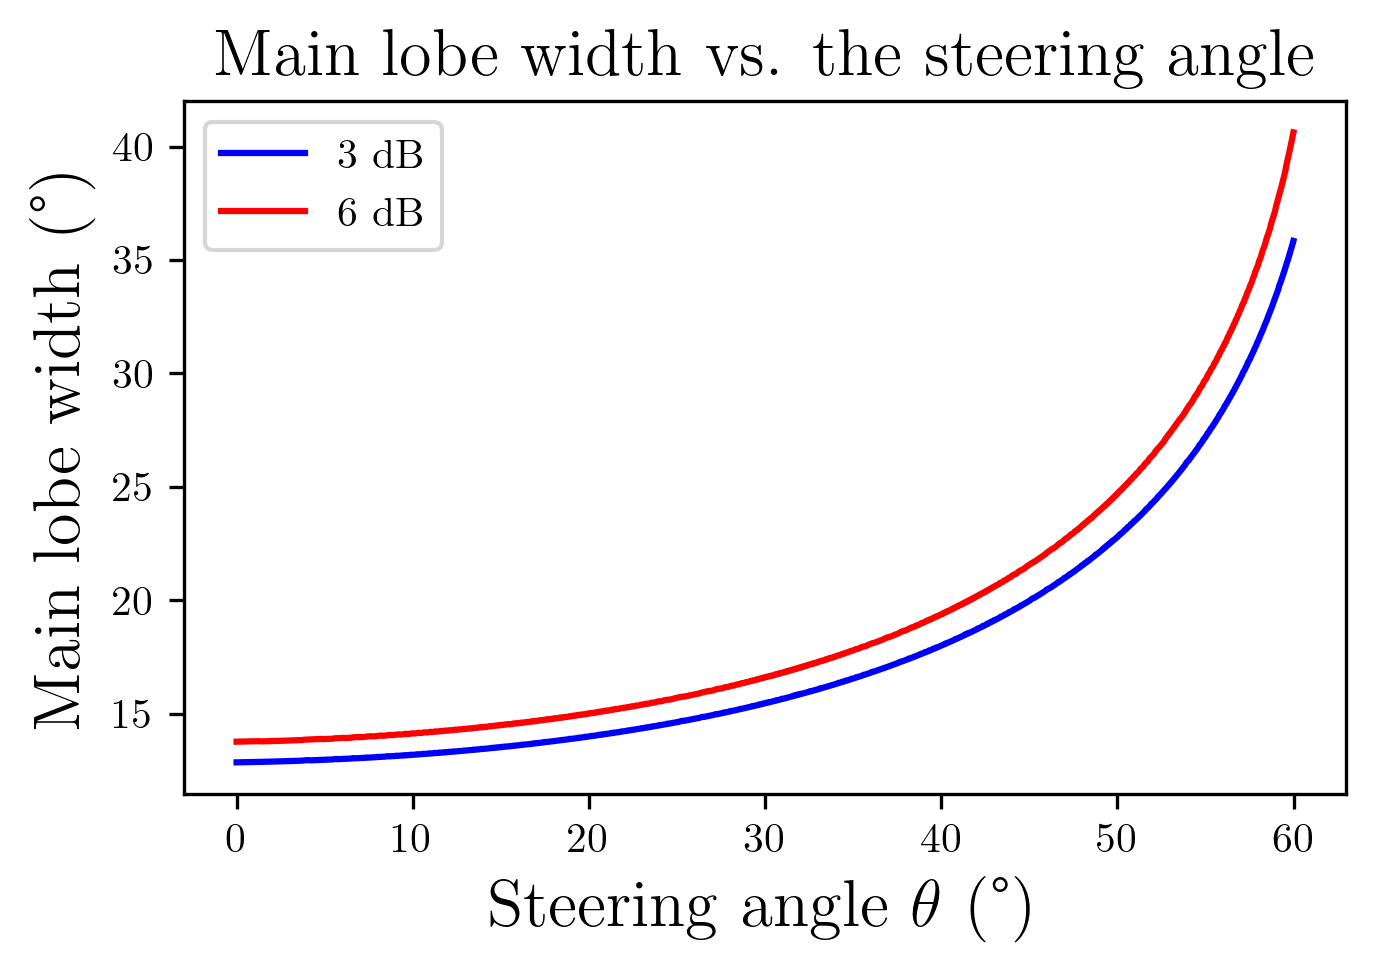
\includegraphics[scale=0.4]{ml_widths_ElPos_theta.png}
				\centering
				\caption{Main lobe width w.r.t $\theta$}
			\end{figure}
			
			
		\end{column}
		
		\begin{column}{0.5\textwidth}
			\vspace{-15pt}
			\begin{figure}
				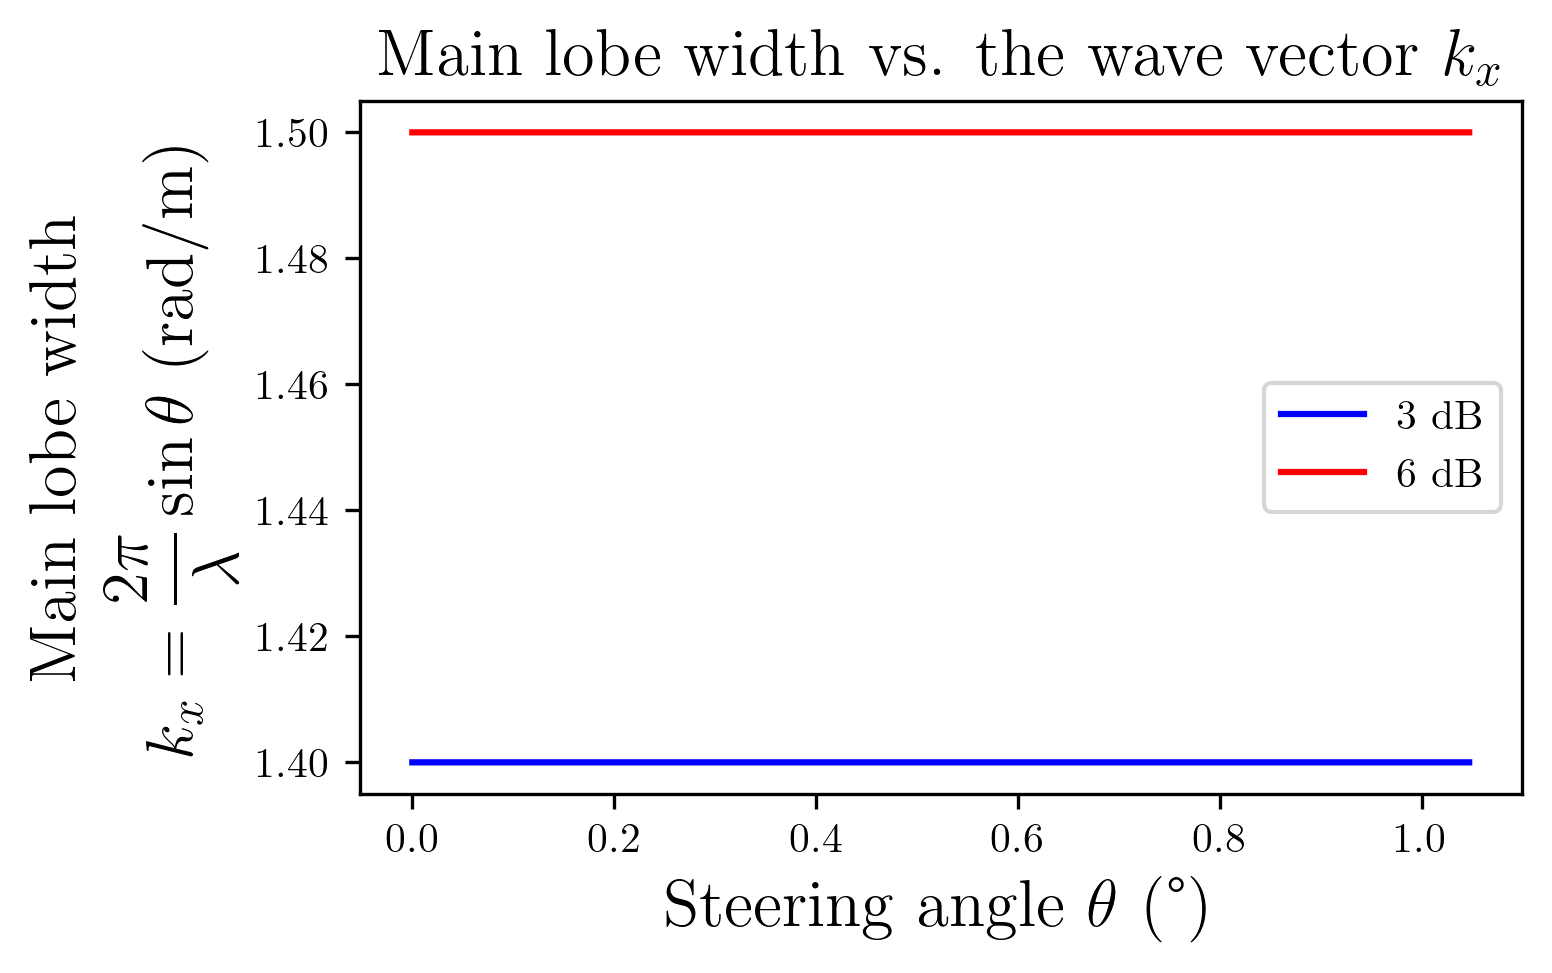
\includegraphics[scale=0.4]{ml_widths_ElPos_k.png}
				\centering
				\caption{Main lobes widths w.r.t $k_x$}
			\end{figure}
		\end{column}
	\end{columns}
\begin{itemize}
	\item Main lobe width w.r.t $\theta$ increases but is constant w.r.t $k_x$\dots Why ?
	\item Steering : $W\left(k_x\right)\rightarrow W\left(k_x-k_x^\circ\right)$ and $W\left(\theta\right)=W\left(\dfrac{2\pi}{\lambda}\sin\theta\right)\rightarrow W\left(\dfrac{2\pi}{\lambda}\sin\theta-\dfrac{2\pi}{\lambda}\sin\theta^\circ\right) $
	\item The array pattern w.r.t $\mathbf{\textcolor{red}{k_x^\circ}}$ is only translated from a constant factor $\implies$ constant main lobe width
		\item The array pattern w.r.t $\textcolor{red}{\mathbf{\theta}}$ is \textbf{\textcolor{red}{shifted and stretched}} 
		\item Why ? Because the beam pattern is a function of \textbf{\textcolor{red}{$\mathbf{\sin\theta}$!}}
		\item Non-linear dependence
		\item Stretching effect varies with $\theta$
		\item For high steering angles, we have large ML
		\item \textcolor{red}{\textbf{Better to tilt the array rather than to steer it\dots}}
\end{itemize}
\end{frame}






	\subsection{Thinning}
	\begin{frame}
		\frametitle{Thinning : uniform distribution \cite{Optimization_of_sparse_arrays}}
		
		
		
		
		\begin{itemize}
			\item Uniform distribution
			\item Results for active elements number $N_{pos}=25,50$ and $75$ 
		\end{itemize} 

	\begin{columns}
	\begin{column}{0.7\textwidth}
			\begin{table}
			\begin{tabular}{ccccccc}
				\hline
				\multirow{2}{*}{Array} &
				\multicolumn{2}{c}{ML 3 \si{\decibel} width(\si{\degree})} &
				\multicolumn{2}{c}{Mean SL level (\si{\decibel})} &
				\multicolumn{2}{c}{Max SL level (\si{\decibel})} \\
				& {Mean} & {Std} & {Mean} & {Std} & {Mean} & {Std} \\
				\hline
				\hline
				$N_{pos}=25$ & $1.02$ & $7.0\times 10^{-2}$ & $-14.1$& $4.6\times 10^{-1}$ & $-7.66$ & $7.6\times 10^{-1}$ \\
				$N_{pos}=50$& $1.01$ & $6.0\times 10^{-2}$ & $-18.3$ & $5.8\times 10^{-1}$ & $-11.53 $& $1.21$\\
				$N_{pos}=75$& $1.01$ & $3.0\times 10^{-2}$ & $-22.5$ & $3.3\times 10^{-1}$ & $-13.77$ & $1.35 $\\
				\hline
			\end{tabular}
			\centering
			\caption{Thinned arrays characteristics (uniform distribution)}
		\end{table}
		
		\begin{table}
			\begin{tabular}{cccc}
				\hline
				Array&ML 3~\si{\decibel} width (\si{\degree})& Mean SL level (\si{\decibel})&Max SL level (\si{\decibel})\\
				\hline\hline
				ULA 101 elements&$1.00$&$ -69.3$ & $-26.5$ \\
				Fig.3 \cite{Optimization_of_sparse_arrays} ($N_{pos}=75$)& $1.19 $& $-13.7$ &$-12.1$\\
				Fig.4 \cite{Optimization_of_sparse_arrays} ($N_{pos}=75$)& $1.46$ & $-14.2$ &$-12.7$\\
					\hline
			\end{tabular}
			\centering
			\caption{Arrays characteristics}
		\end{table}
		
	\end{column}
	
	\begin{column}{0.3\textwidth}
		\textbf{Analysis (other arrays):}
		\begin{itemize}
			\item ULA and thinned arrays have the \textcolor{red}{\textbf{same ML width}}
			\item But \textcolor{red}{\textbf{higher SL}} for thinned arrays
			\item Thinned arrays have \textcolor{red}{\textbf{lower SL}} than the arrays presented in \cite{Optimization_of_sparse_arrays}
		\end{itemize}
		\textbf{Analysis ($N_{pos}$): }
		\begin{itemize}
			\item ML width remains \textcolor{red}{\textbf{ constant}} when $N_{pos}$~$\nearrow$
			\item Both SL max and mean level $\searrow$
			\item Variance is decreasing
			\item Thinned array $\xrightarrow[N_{pos} \to M]{}$ ULA
			\item \textcolor{red}{\textbf{Reduced sensitivity to signal coming from directions}} $\theta\neq 0$
		\end{itemize}
		
	\end{column}
\end{columns}

\begin{itemize}
	\item Remark : using thinned arrays reduces the white Gaussian noise! We are only using $N_{pos}$ elements! $\left(\rVert w\rVert^{-2} = N_{pos}\right)$
\end{itemize}
		
	

\end{frame}


	\begin{frame}
	\frametitle{Thinning : Gaussian distribution \cite{Optimization_of_sparse_arrays}}
	
	
	
	
	
	
	
	\begin{columns}

		
		
		\begin{column}{0.7\textwidth}
			\begin{itemize}
				\item Gaussian distribution
				\item Results for active elements number $N_{pos}=25,50$ and $75$ 
				\item Standard deviation : $\dfrac{N_{els}}{6}\approx 16.83$
			\end{itemize} 
			\begin{table}
				\begin{tabular}{lSSSSSS}
					\hline
					\multirow{2}{*}{Array} &
					\multicolumn{2}{c}{ML 3 \si{\decibel} width(\si{\degree})} &
					\multicolumn{2}{c}{Mean SL level (\si{\decibel})} &
					\multicolumn{2}{c}{Max SL level (\si{\decibel})} \\
					& {Mean} & {Std} & {Mean} & {Std} & {Mean} & {Std} \\
					\hline
					\hline
					$N_{pos}=25$ & 1.43 & 0.14 & -15.07& 0.74 & -8.47 & 0.86 \\
					$N_{pos}=50$& 1.42 & 0.07 & -20.45 & 0.67 & -13.82 & 0.87 \\
					$N_{pos}=75$& 1.22 & 0.03 & -24.54 & 0.59 & -18.17 & 1.05 \\
					\hline
				\end{tabular}
				\centering
				\caption{Thinned arrays characteristics (Gaussian distribution, std $\approx 16.8$ elements)}
			\end{table}
			
			\begin{table}
			\begin{tabular}{cccc}
				\hline
				Array&ML 3~\si{\decibel} width (\si{\degree})& Mean SL level (\si{\decibel})&Max SL level (\si{\decibel})\\
				\hline\hline
				ULA 101 elements&1.0& -69.3 & -26.5 \\
				Fig.3 \cite{Optimization_of_sparse_arrays} ($N_{pos}=75$)& 1.19 & -13.7 & -12.1\\
				Fig.4 \cite{Optimization_of_sparse_arrays} ($N_{pos}=75$)& 1.46 & -14.2 & -12.7\\
				\hline
			\end{tabular}
			\centering
			\caption{Arrays characteristics}
		\end{table}
			
		\end{column}
		
		\begin{column}{0.25\textwidth}
			\textbf{Analysis vs. other arrays :}
			\begin{itemize}
				\item Wider ML and lower SL than the thinned array with a uniform distibution
				\item \textcolor{red}{\textbf{Larger ML and higher SL}} than the ULA
				\item \textcolor{red}{\textbf{Lower SL}} than the arrays presented in \cite{Optimization_of_sparse_arrays}...
				\item Using a gaussian distribution for the elements position is equivalent to use a Gaussian distibution for the weights : spatial tapering $\Longleftrightarrow$ amplitude tapering 
			\end{itemize}
			\textbf{Analysis ($N_{pos}$) : }
			\begin{itemize}
				\item ML width decreases when $N_{pos}$~$\nearrow$
				\item Both SL max and mean level $\searrow$
			\end{itemize}
			
		\end{column}
	\end{columns}
	
	
	
	
	
\end{frame}

\begin{frame}
	\frametitle{Binned sparse array  \cite{Sampling_theory}}


	\begin{columns}
	
	\begin{column}{0.7\textwidth}
How to design a binned spare array?
\begin{itemize}
	\item We consider an array with $M=101$ sensors with element spacing $d=\dfrac{\lambda}{2}$
	\item The size of the array is $L=(M-1)d$
	\item We divide it into $N$ bins of size $w=\dfrac{L}{N}$
	\item The position of the $m$-th element is given by $x_m = -\dfrac{L}{2} + m\cdot w + y_m$ where $y_m$ is drawn from $\mathcal{U}_{[0,1]}$
\end{itemize}
	\end{column}
	
	\begin{column}{0.3\textwidth}
		\begin{figure}[h!]
			\vspace{-25pt}
			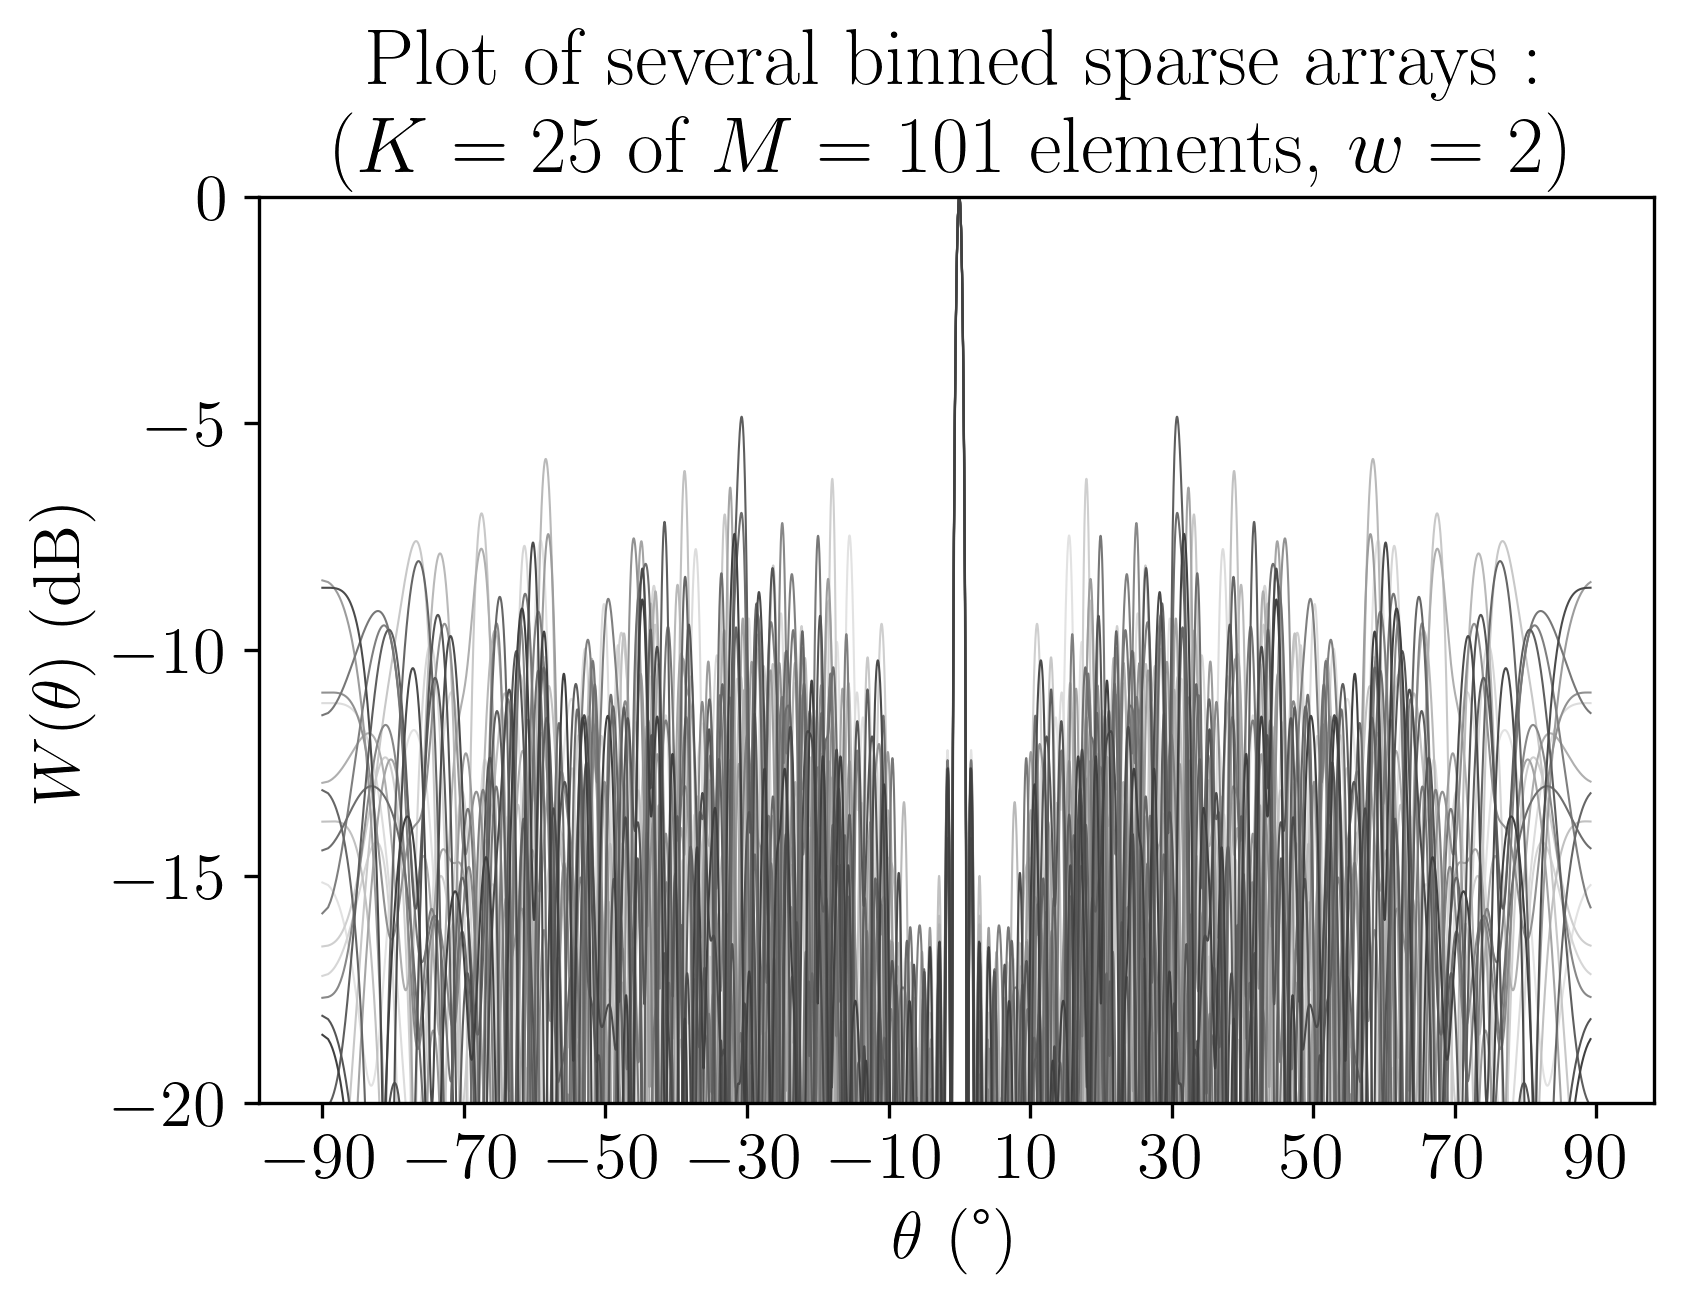
\includegraphics[scale=0.3]{binned_spare_array.png}
			\vspace{-8pt}
			\caption{Binned spare arrays}
			\centering
			\vspace{-25pt}
		\end{figure}
\end{column}
\end{columns}

		\begin{table}
			\begin{tabular}{ccccccc}
				\hline
				\multirow{2}{*}{Array} &
				\multicolumn{2}{c}{ML 3 \si{\decibel} width(\si{\degree})} &
				\multicolumn{2}{c}{Mean SL level (\si{\decibel})} &
				\multicolumn{2}{c}{Max SL level (\si{\decibel})} \\
				& {Mean} & {Std} & {Mean} & {Std} & {Mean} & {Std} \\
				\hline
				\hline
				$N_{pos}=25$ (from \cite{Nonuniformly_spaced_linear}) & $1.0$ & $7.0\times 10^{-2}$ & $-14.1$& $4.6\times 10^{-1}$ & $-7.66$ & $7.6\times 10^{-1}$ \\
				$K=25$ (from \cite{Sampling_theory})&$1.0$&$1.0\times 10^{-2}$&$-14.8$&$5.0\times 10^{-1}$&$-6.73$&$1.01$\\
				\hline
			\end{tabular}
			\centering
			\caption{Thinned array with uniform distribution vs. binned spare array}
		\end{table}
\textbf{Analysis}
		\begin{itemize}
			\item Same ML width but \textcolor{red}{\textbf{lower variance}} for the binned spare array
			\item "This means that the binned array has a much larger region around the steered direction where the effect of the randomness is small" \cite{Sampling_theory}
			\item SL mean and max levels are \textcolor{red}{\textbf{similar}}
			\item\textbf{Different aperture} : for the binned spare array, the $\implies$ $K$ first elements are \textcolor{red}{\textbf{jittered}}; for the thinned array, outer elements are conserved
		\end{itemize}
\end{frame}





	\subsection{Element directivity}
	\begin{frame}
		\frametitle{Element directivity}
		
			\begin{columns}
			
			\begin{column}{0.4\textwidth}
			\vspace{-15pt}
			\begin{figure}[h!]
				\centering
				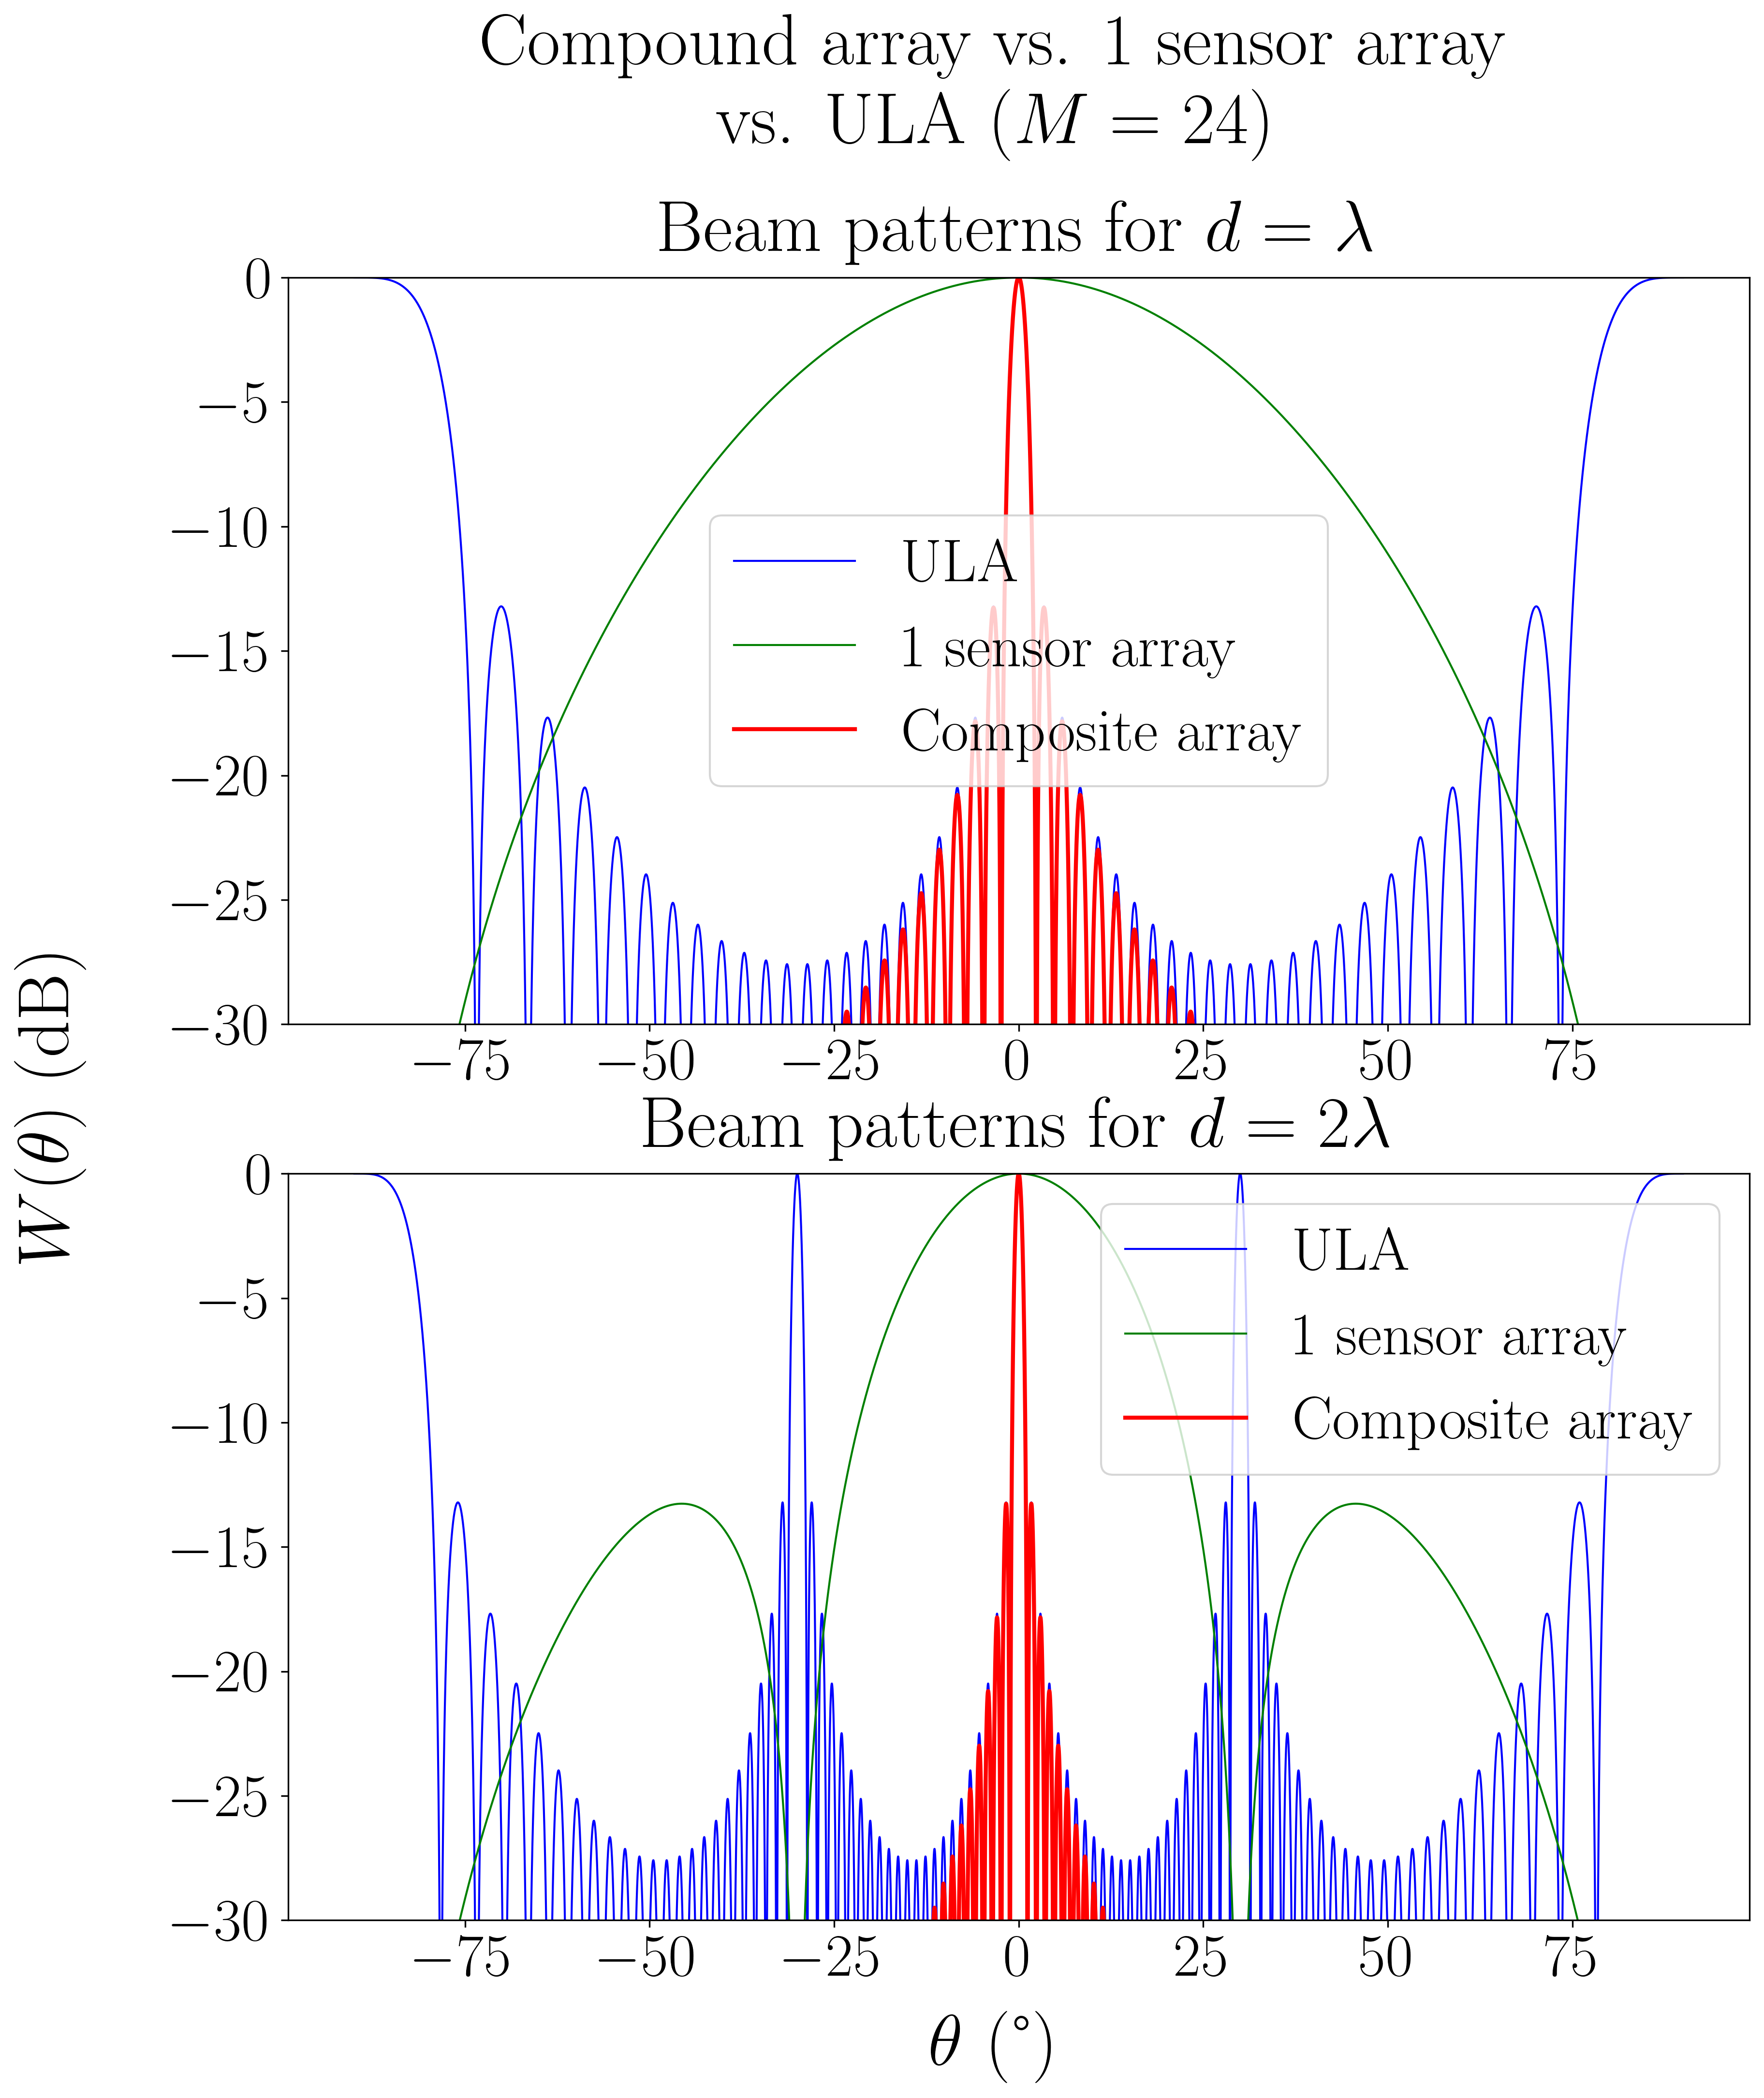
\includegraphics[scale=0.2]{compound_vs_ula_1sensor_patterns_deg.png}
				\caption{Composite arrays for $d=\lambda$ and $d=2\lambda$}
			\end{figure}
	
				
			\end{column}
			
			\begin{column}{0.6\textwidth}
				\vspace{-20pt}
			\begin{figure}[h!]
				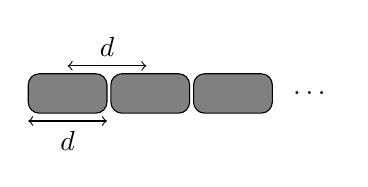
\begin{tikzpicture}[scale=1]
					\draw [fill=gray,rounded corners] (0,0) rectangle (1,0.5);
					\draw [<->](0,-0.1)--(1,-0.1);
					\draw (0.5,-0.1) node [below]{$d$};
					\draw [<->](0.5,0.6)--(1.5,0.6);
					\draw (1,0.6) node [above]{$d$};
					\draw [fill=gray,rounded corners](1.05,0) rectangle (2.05,0.5);
					\draw (3.6,0.25) node {\dots};
					\draw [fill=gray,rounded corners](2.1,0) rectangle (3.1,0.5);
				\end{tikzpicture}
			\centering
			\caption{Composite array}
			\end{figure}
			\begin{itemize}
				\item Composite array : $M$ sensors of size $d$ with element spacing $d$, unity weights
				\item $d>\dfrac{\lambda}{2}$ : \textcolor{red}{\textbf{ULA sampling criterion}} (and also \textsc{NYQUIST's} sampling theorem) is not verified \textcolor{red}{\faTimes}$\implies$ grating lobes + aliasing for the ULA 
				\item Composite arrays : low SL levels \textcolor{green}{\faCheck}
				\item And no grating lobes
				\item Composite array beam pattern perfectly fits the ULA ML for both element spacings!
				\item So, using composite arrays reduces the sensitivity in directions $\theta\neq 0$ while keeping a good resolution. But what about steering?
			\end{itemize}
			\end{column}
	
		\end{columns}
			\end{frame}
		
		\begin{frame}
			\frametitle{Steered composite array}
			
	\begin{columns}
	
	\begin{column}{0.37\textwidth}
\vspace{-15pt}
\begin{figure}[h!]
	\centering
	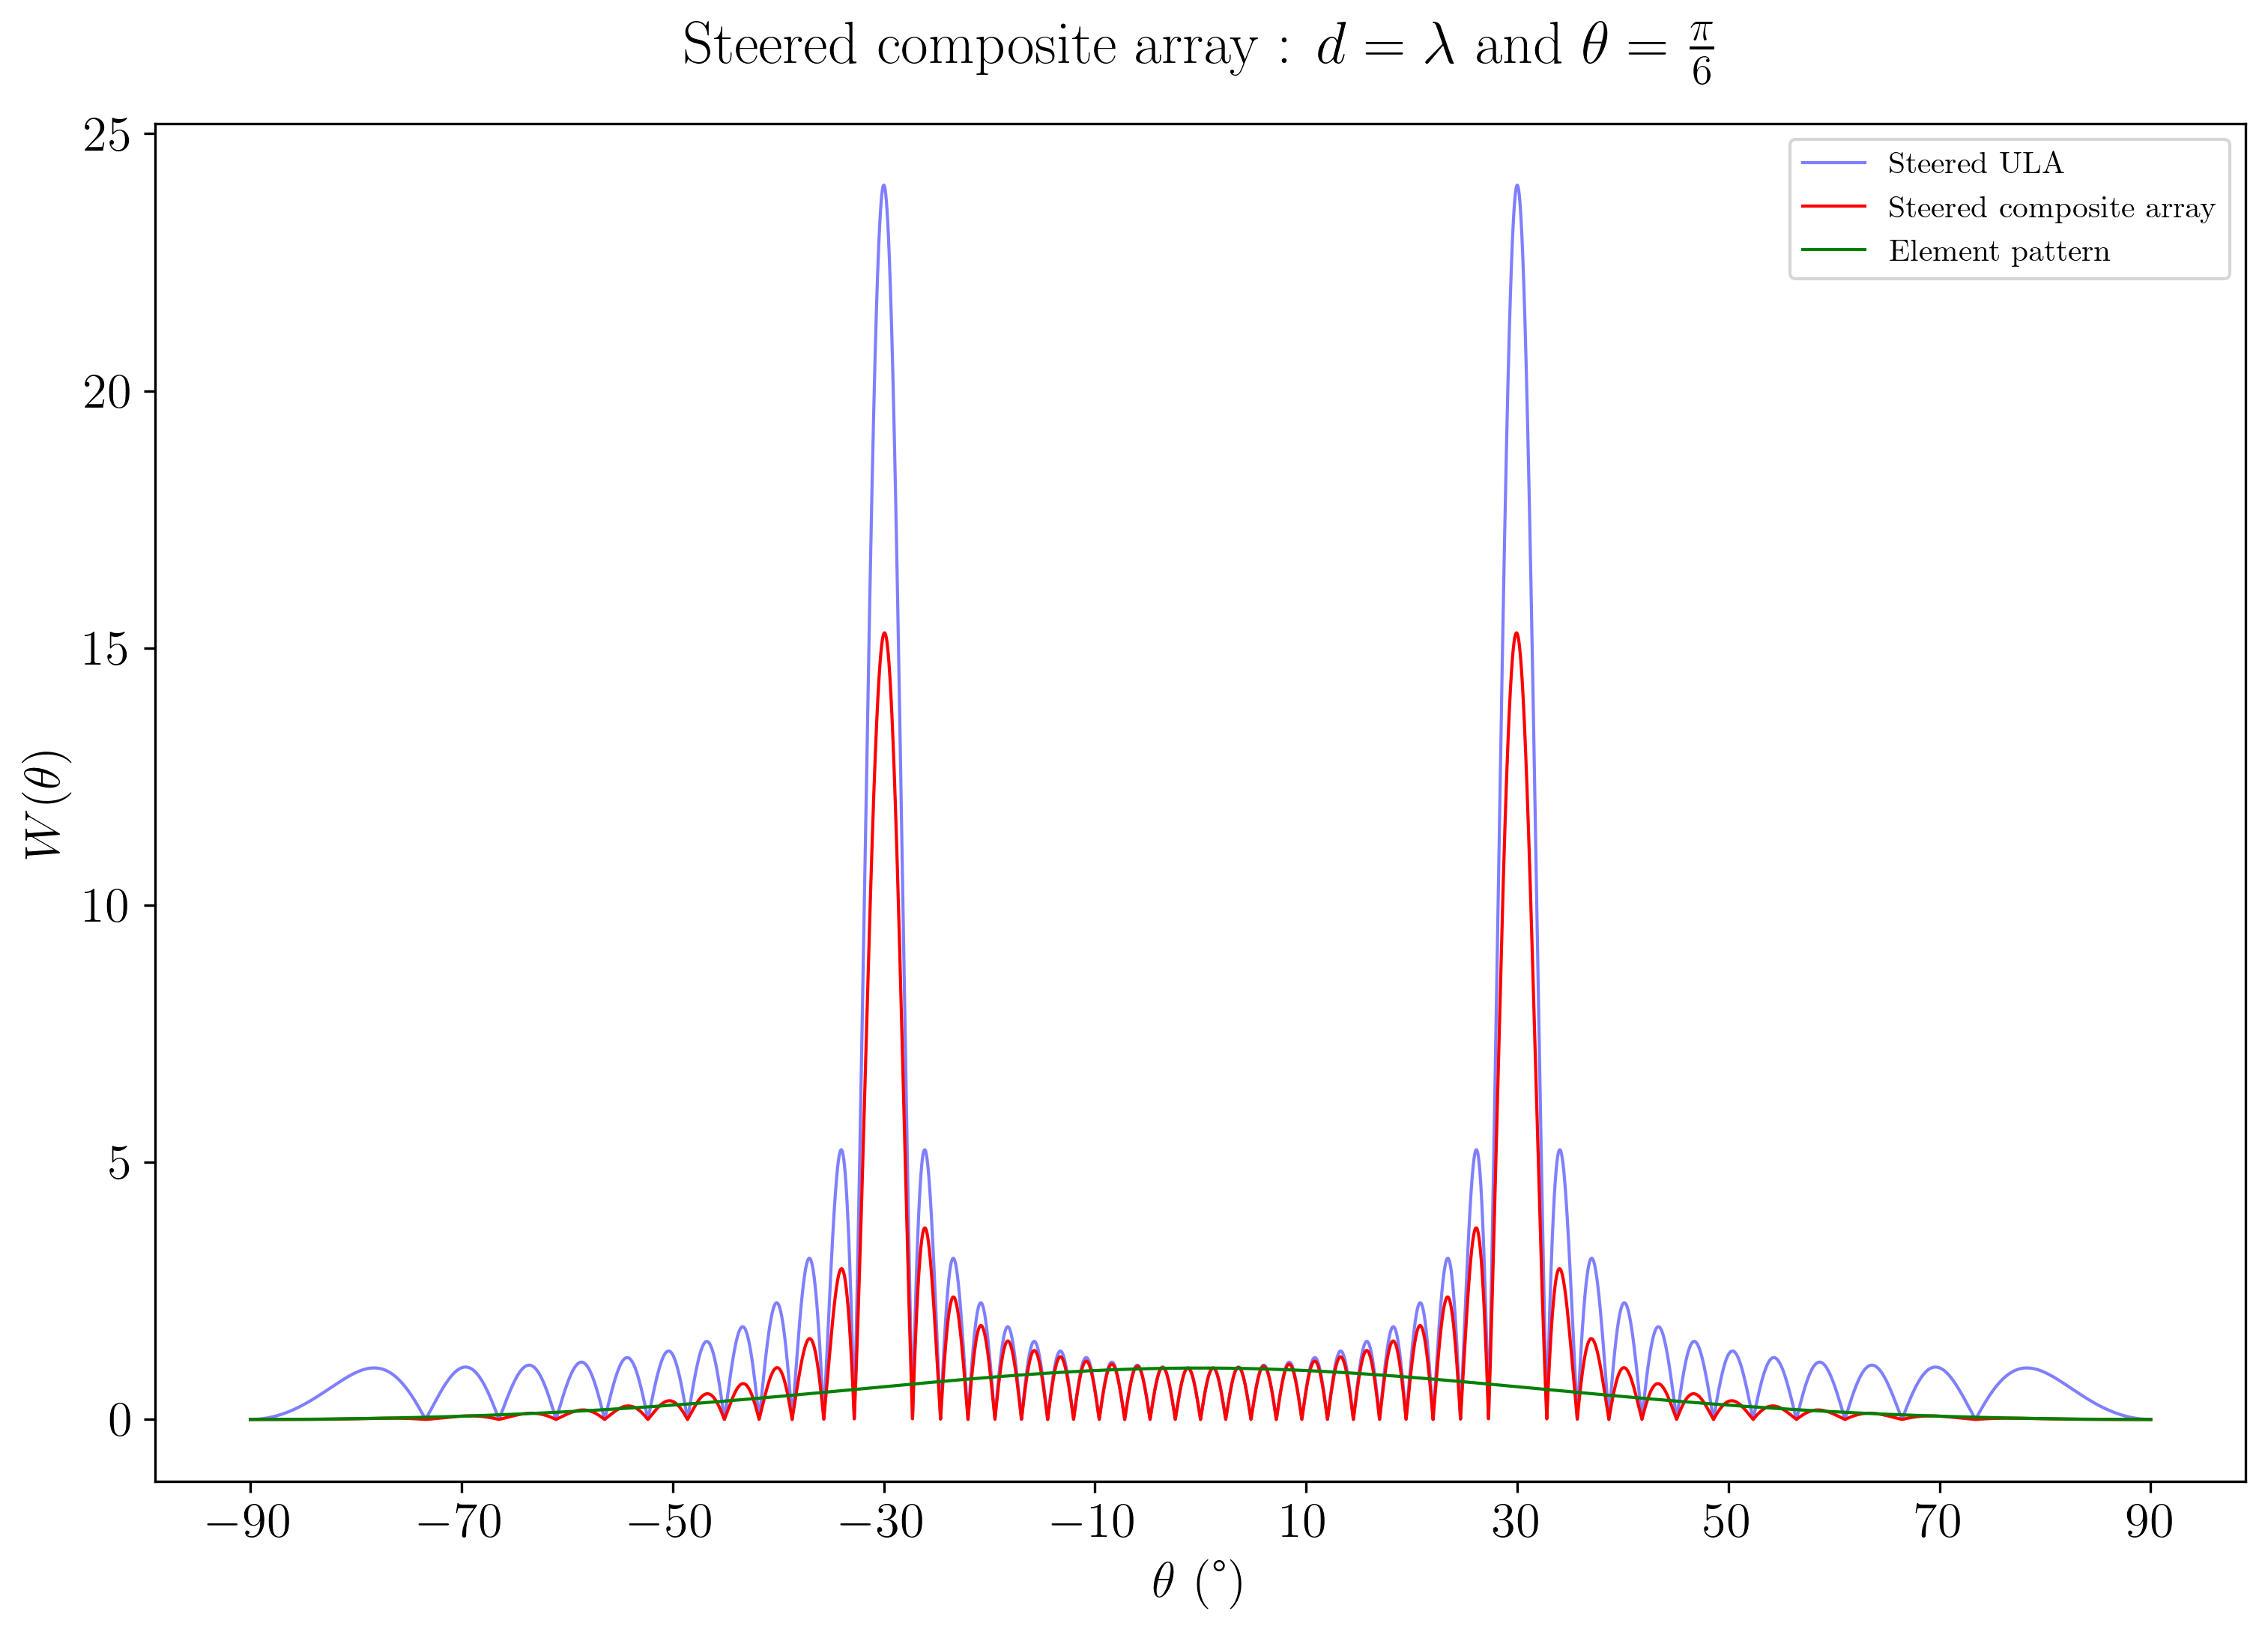
\includegraphics[scale=0.2]{steered_compound_array_description.png}
	\caption{Steered compound array}
\end{figure}
	\end{column}
	
	\begin{column}{0.63\textwidth}
	\vspace{-15pt}
	\begin{figure}[h!]
		\centering
		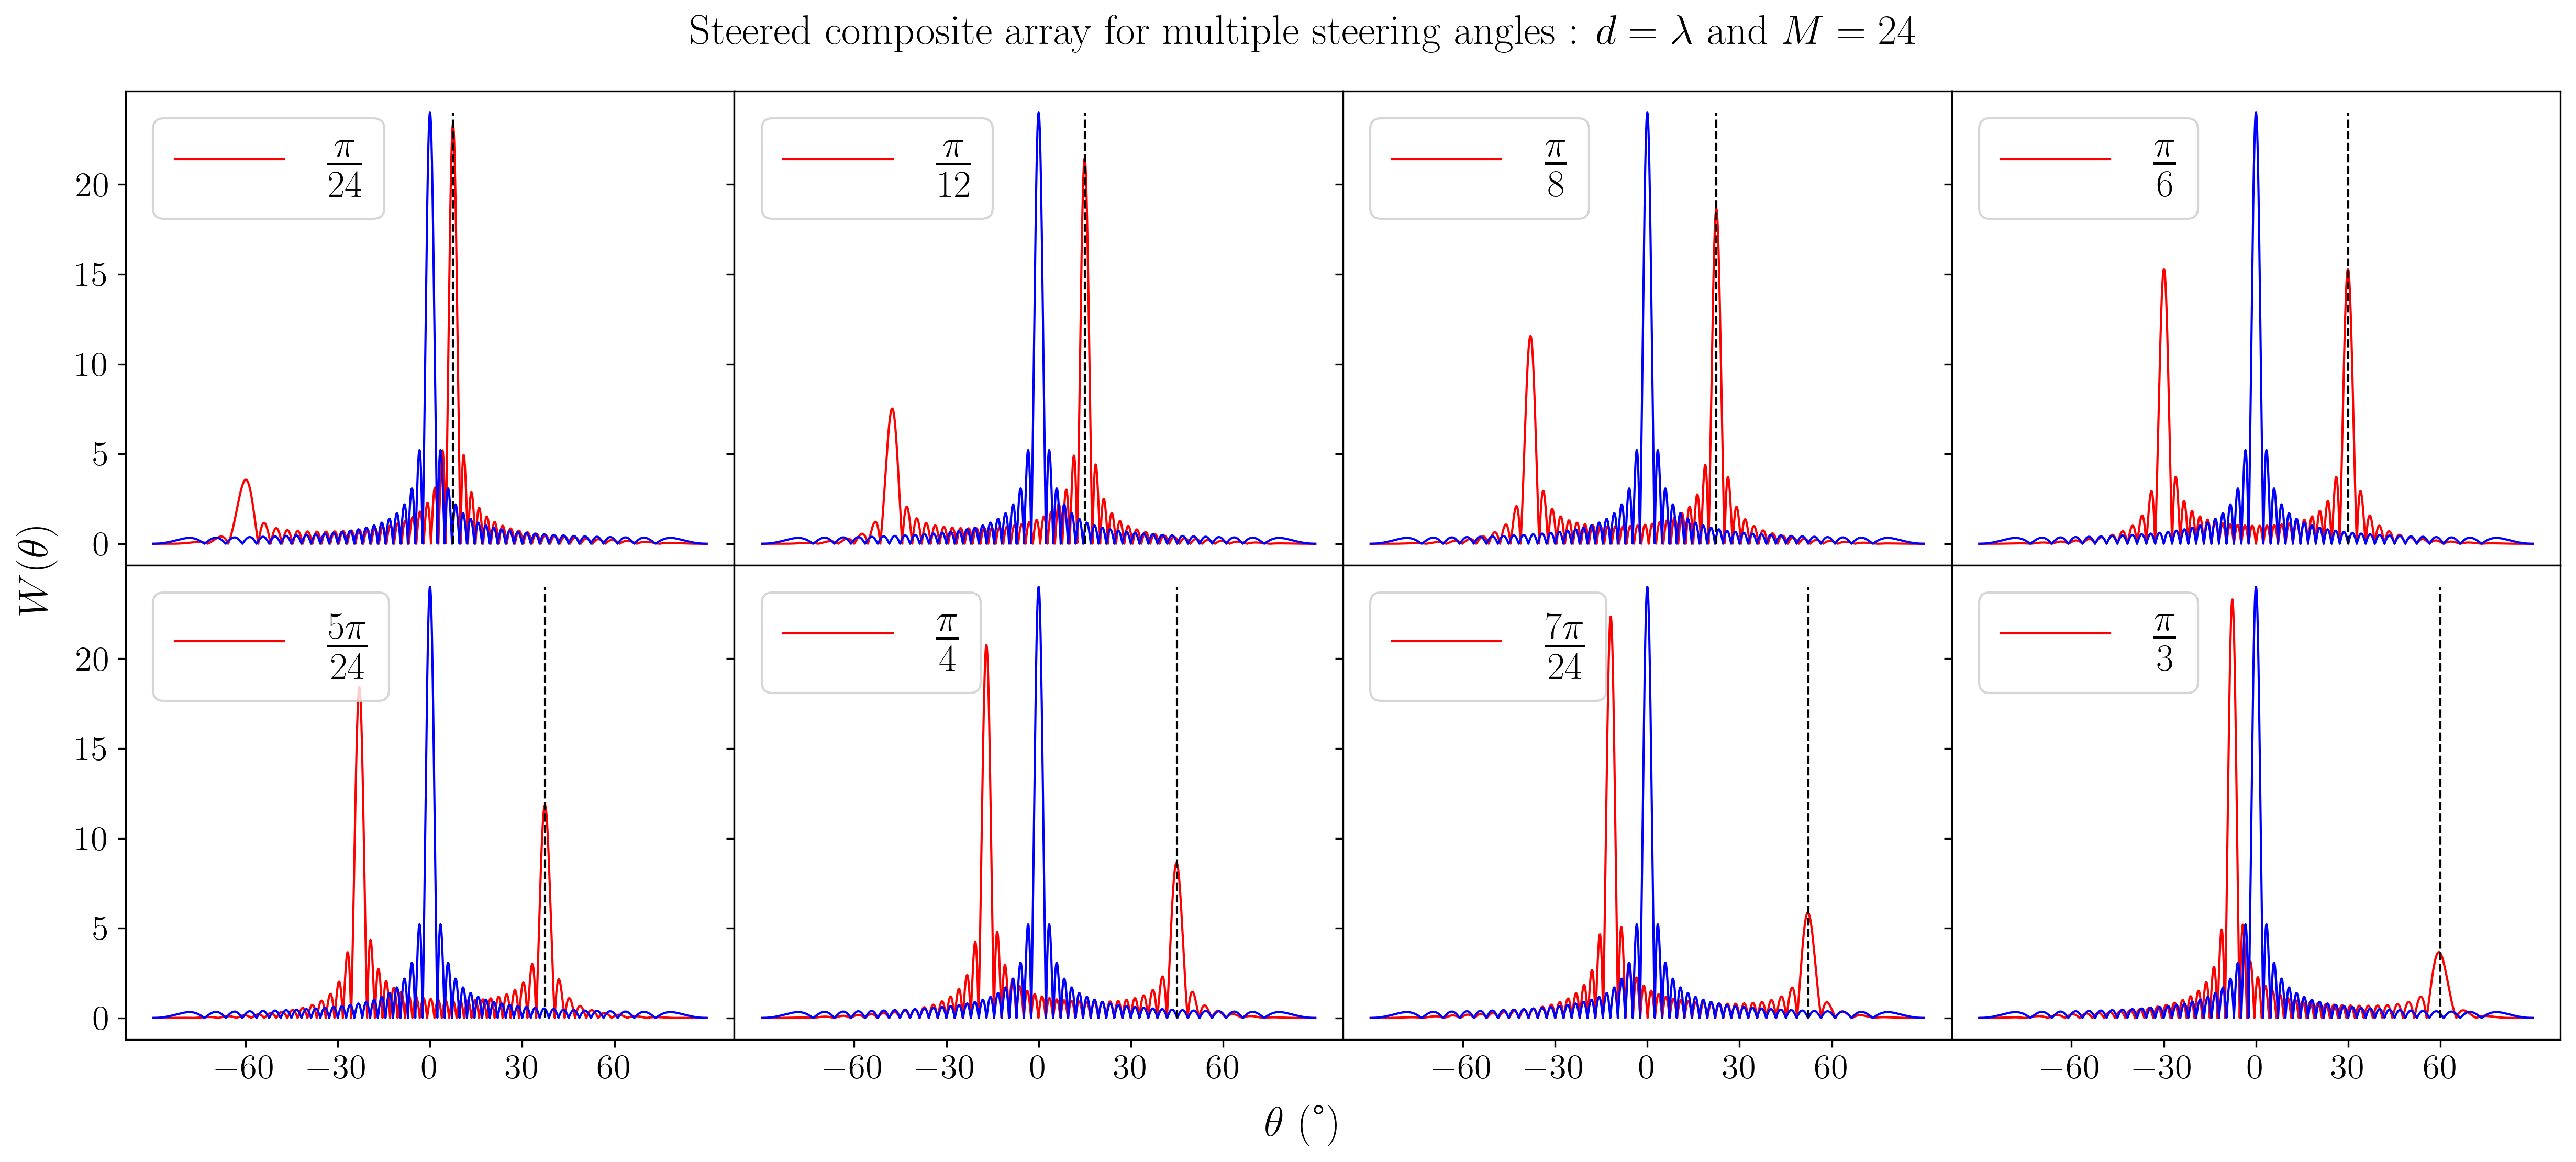
\includegraphics[scale=0.2]{steered_composite_arrays_multiple_steering_angles.png}
		\caption{Steered composite array pattern for multiple steering angles}
	\end{figure}
	\end{column}
\end{columns}

\begin{itemize}
	\item As the steering angle increases :
	\item A \textcolor{red}{\textbf{grating lobe}} appears
	\item And the \textcolor{red}{\textbf{side lobes}} (w.r.t the main lobe level) levels \textcolor{red}{\textbf{increase}}
	\item For high value of the steering angle, the grating lobe \textcolor{red}{\textbf{replaces}} the main lobe
	\item This composite array is unsuitable for high steering angle values!
\end{itemize}
		\end{frame}
	
\begin{frame}
	\frametitle{Linear array design}
	\vspace{-10pt}
	\begin{figure}[h!]
		\centering
		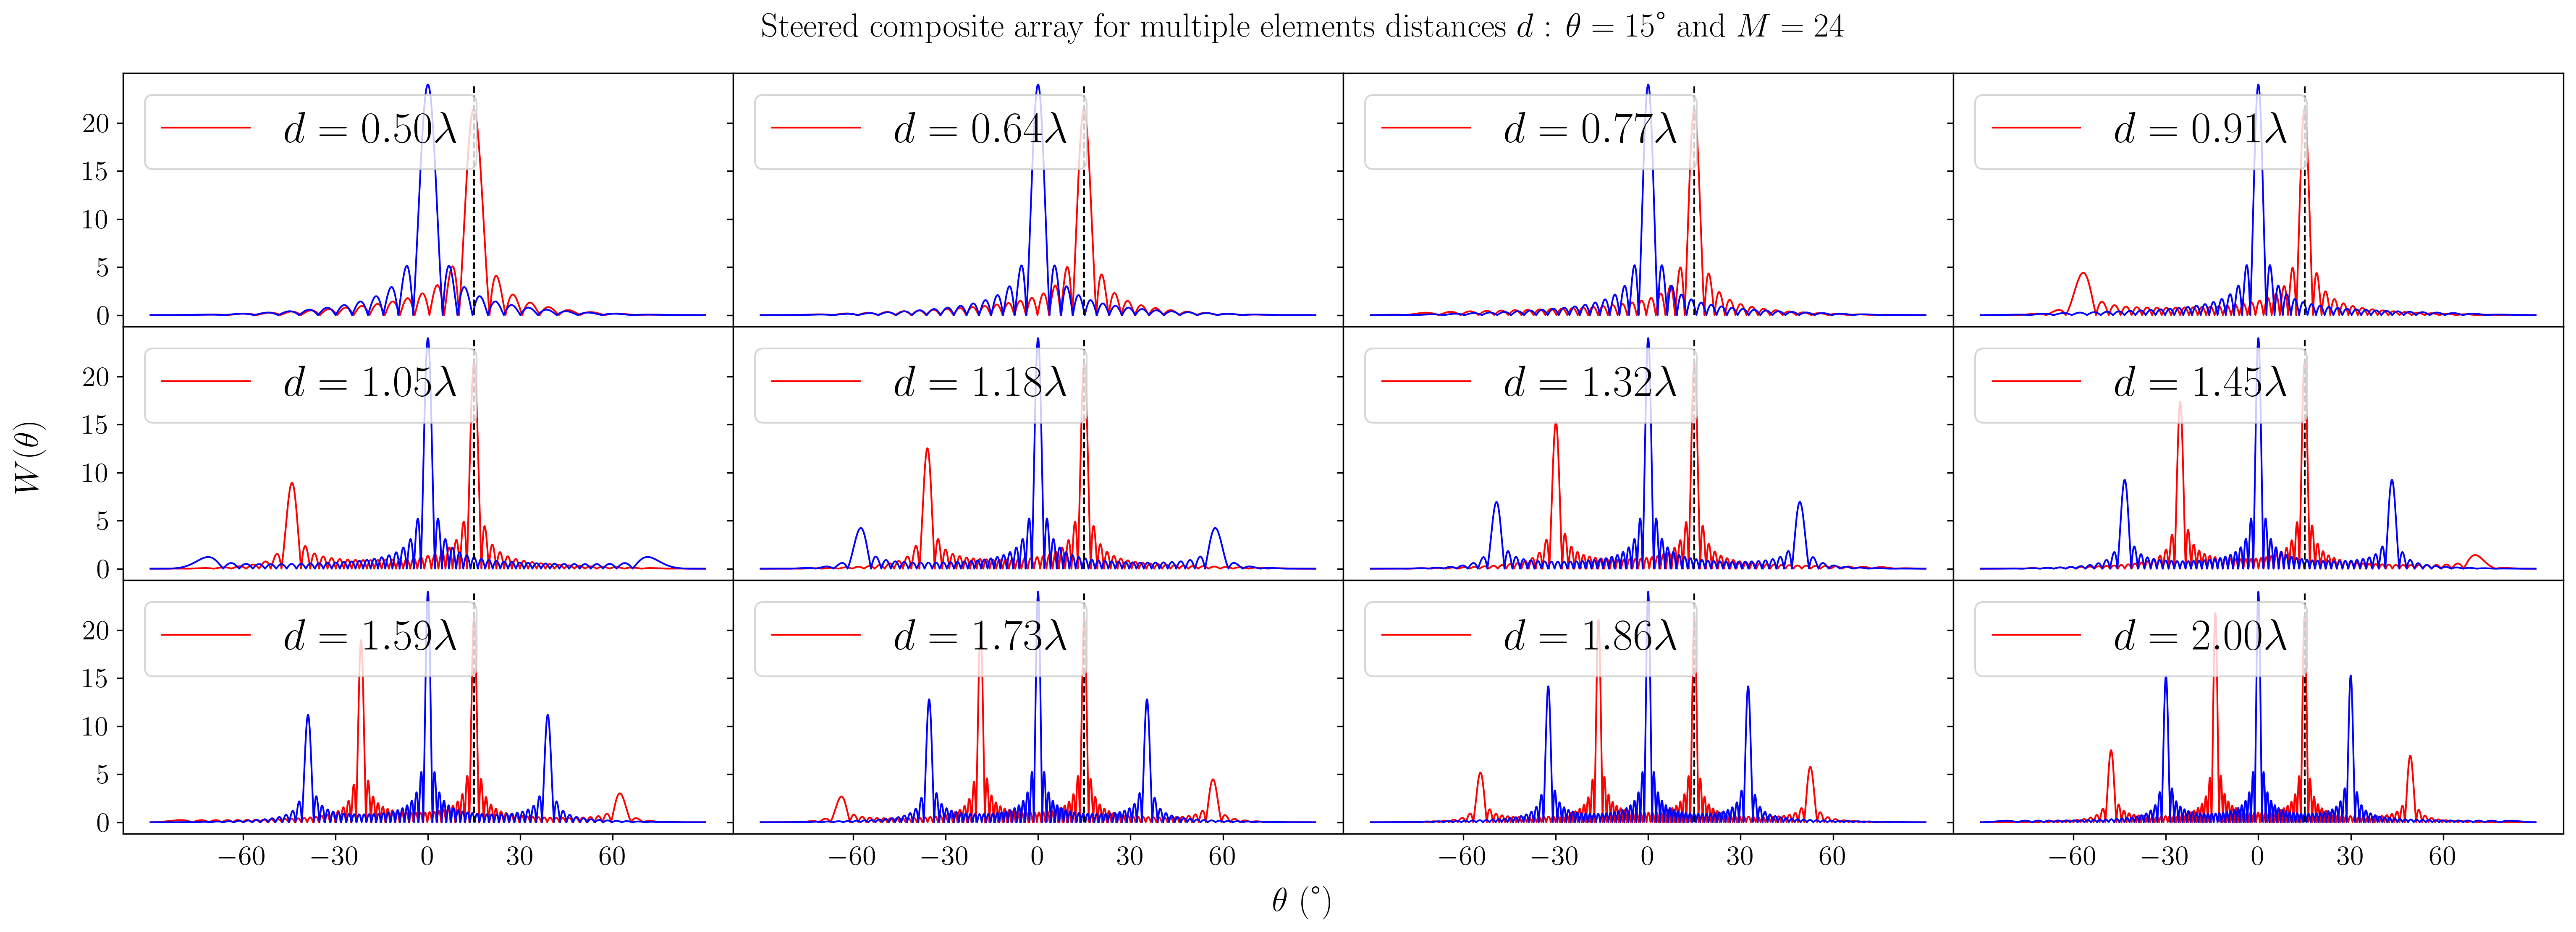
\includegraphics[scale=0.27]{steered_composite_arrays_multiple_distance.png}
		\caption{Steered composite array pattern for multiple elements distances}
	\end{figure}
\begin{itemize}
	\item Acceptable grating lobes levels?
	\item \textcolor{red}{\textbf{Should be less or equal to the half main lobe level}}
	\item For $d\geq1.32\lambda$ : the grating lobe level is too high
	\item $d=1.05\lambda$ and $d=1.18\lambda$ seem to be good trade-off between aperture and grating lobes levels
\end{itemize}
\end{frame}

\begin{frame}
	\frametitle{References \& additional figures}
		\begin{columns}
		
		\begin{column}{0.5\textwidth}
			\vspace{-15pt}
			\begin{figure}[h!]
			\centering
			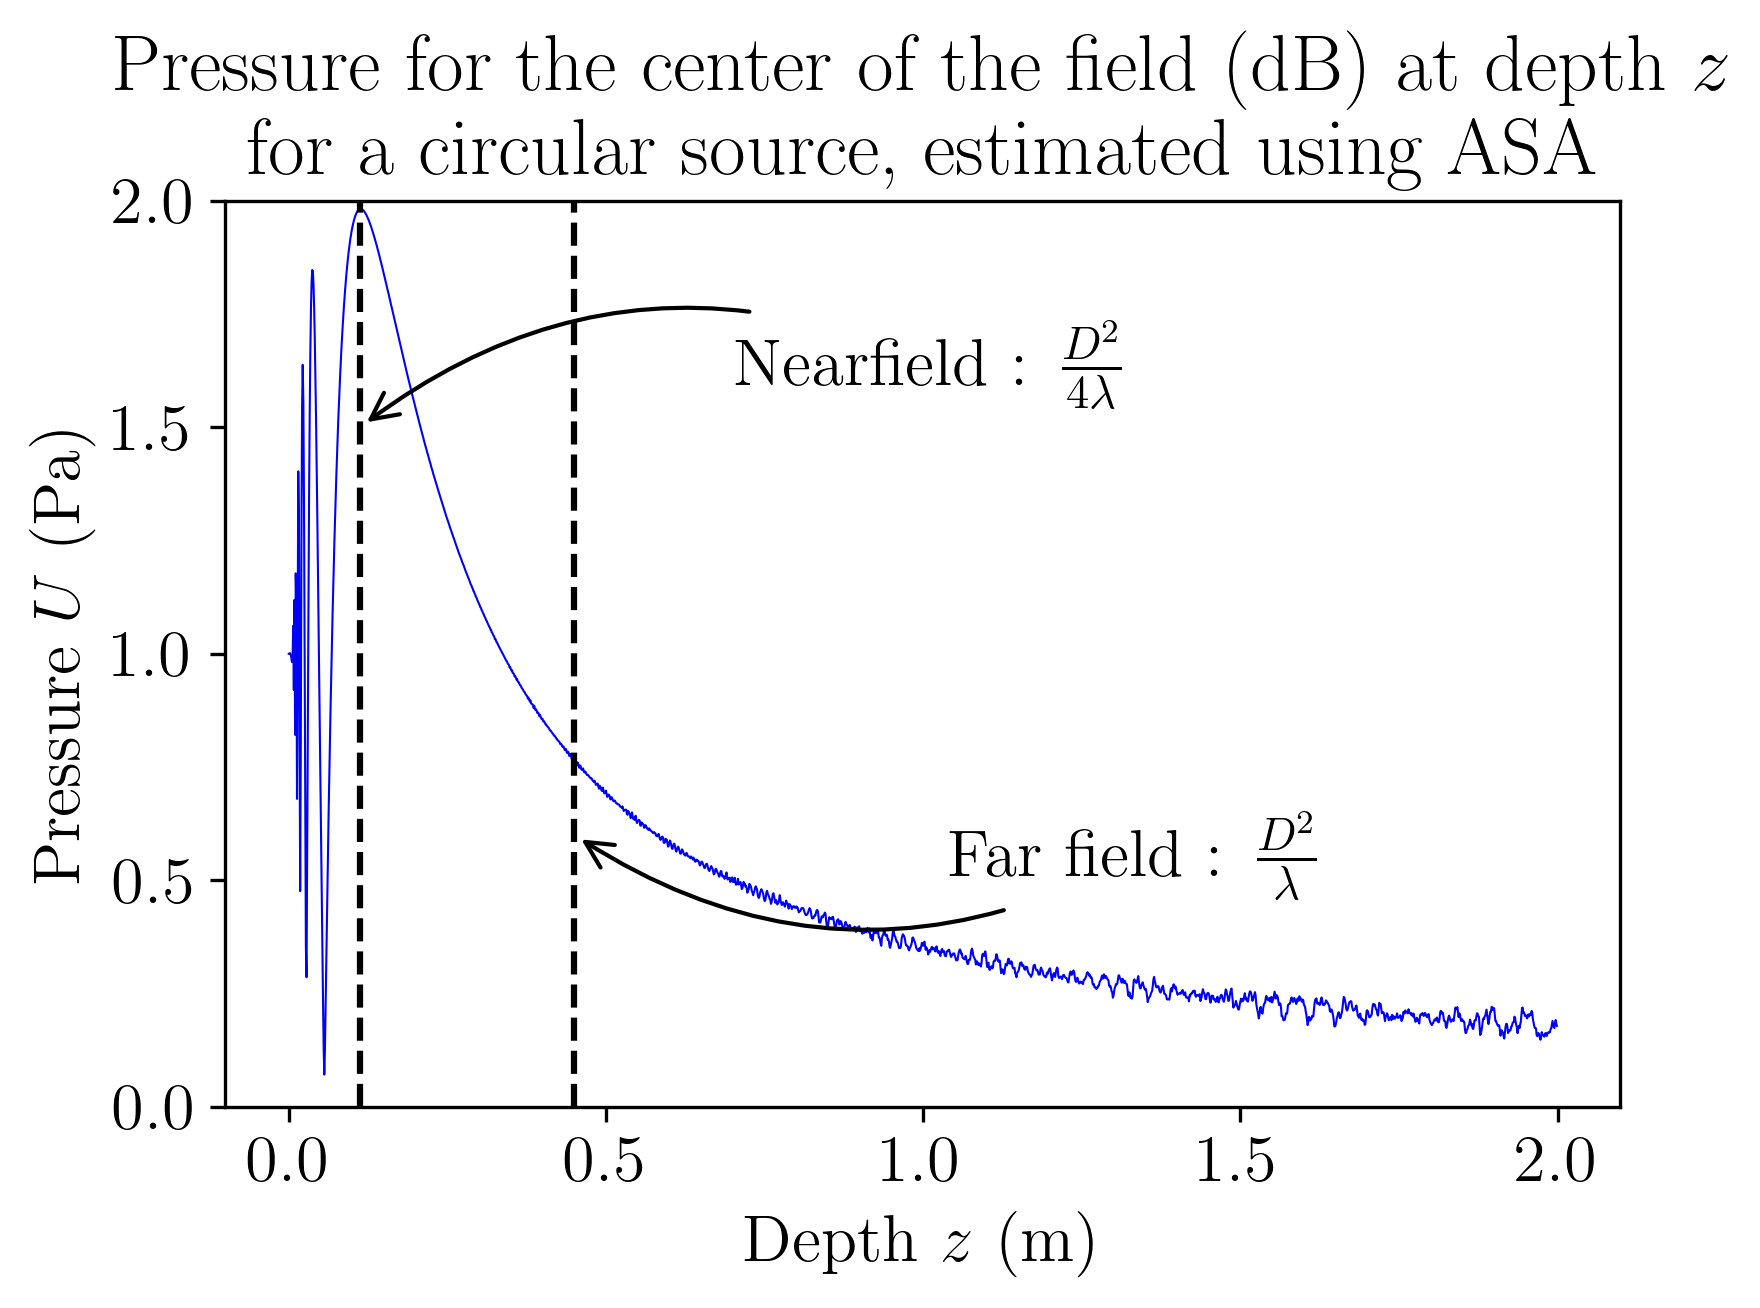
\includegraphics[scale=0.35]{circular/wave_field_1D_center_circular_smoothed.png}
			\caption{Pressure at the wave field center (circular source)}
		\end{figure}
		\end{column}
		
		\begin{column}{0.5\textwidth}
			\vspace{-15pt}
			\begin{figure}[h!]
				\centering
				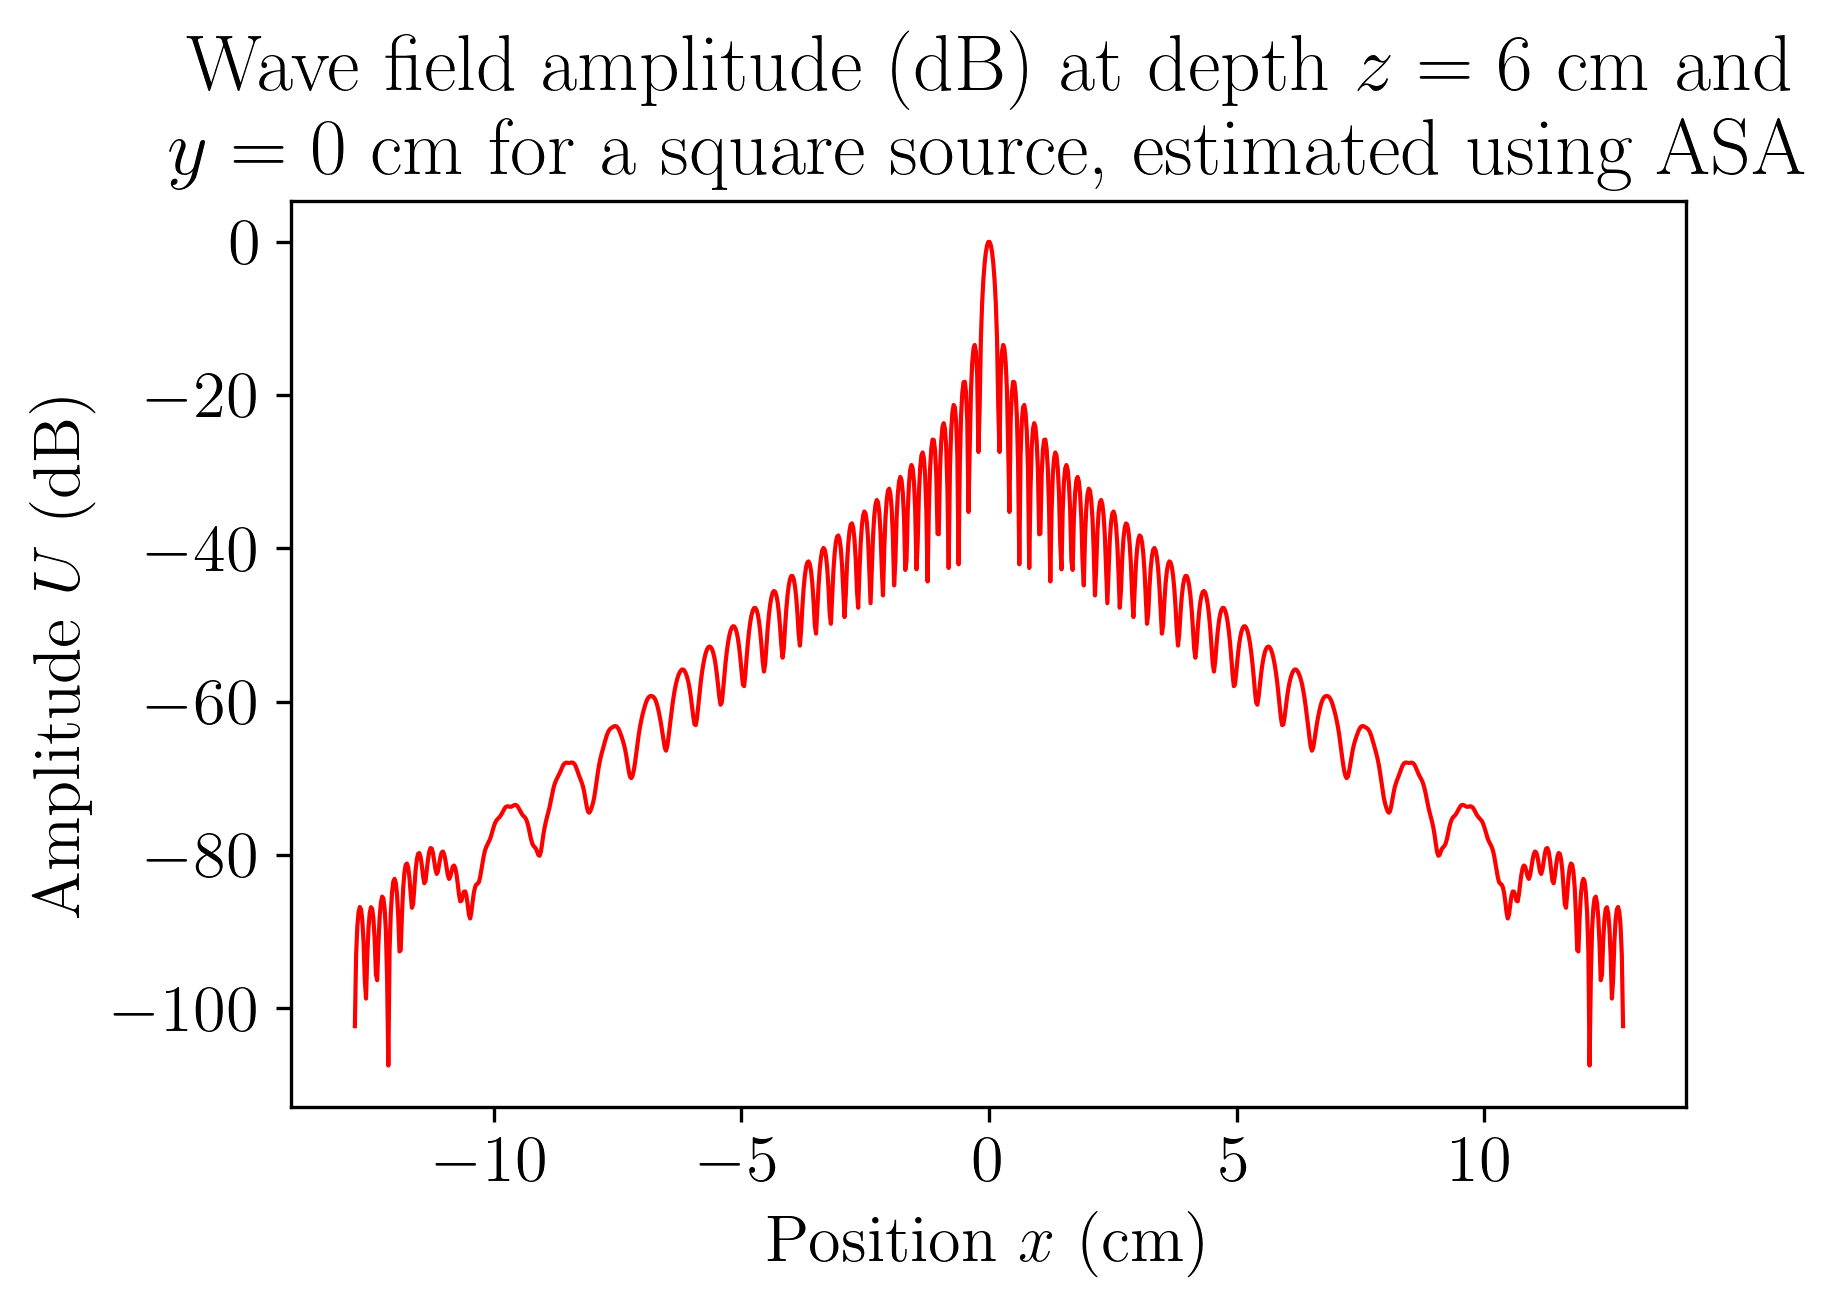
\includegraphics[scale=0.35]{square/wave_field_1D_z=6cm_square_focused}
				\caption{Wave field center cut at the focusing point (square source)}
			\end{figure}
		\end{column}
	\end{columns}
	\printbibliography
\end{frame}




\end{document}